\documentclass[11pt, openany]{book}

% --- Core Packages ---
\usepackage[paperwidth=5.5in, paperheight=8.5in, margin=0.75in]{geometry} % Standard Trade Paperback
\usepackage[T1]{fontenc}
\usepackage{ebgaramond}
\usepackage{FiraMono}
\usepackage[scale=0.9]{inter}



\usepackage{titlesec}
\usepackage{enumitem}
\usepackage{xcolor}
\usepackage{graphicx}
\usepackage{tikz}
\usepackage{setspace}
\usepackage{fancyhdr}
\usepackage{csquotes}
\usepackage{url}
\usepackage{pdfpages} % Allows full-page image insertion
\usepackage{eso-pic} % For absolute positioning of elements
\usepackage{hyperref}

% --- Custom Colors (Metabolic Palette) ---
\definecolor{collectiveBlue}{HTML}{0070FF}
\definecolor{legacyGrey}{HTML}{4D4D4D}
\definecolor{signalGold}{HTML}{FFD700}

% --- Typography ---
 % Elegant, classical serif for prose

\newcommand{\monofont}{\ttfamily} % For AR/System data strings

\newcommand{\headerfont}{\sffamily} % Modern sans-serif for system elements

% --- Chapter Styling ---
\titleformat{\chapter}[display]
  {\headerfont\bfseries\huge\color{legacyGrey}}
  {\filleft\headerfont\fontsize{60}{60}\selectfont\color{gray!20}\thechapter}
  {1ex}
  {\titlerule\vspace{1ex}\filright}

% --- Custom Environments ---

% 1. The Epigraph (At the start of chapters)
\newcommand{\epigraph}[2]{
    \begin{flushright}
    \begin{minipage}{0.7\textwidth}
        \begin{flushright}
        \itshape\small #1 \\
        \vspace{0.5ex}
        \headerfont\upshape\scriptsize #2
        \end{flushright}
    \end{minipage}
    \end{flushright}
    \vspace{4ex}
}

% --- Header/Footer ---
\pagestyle{fancy}
\fancyhf{}
\fancyhead[LE,RO]{\headerfont\scriptsize\thepage}
\fancyhead[RE]{\headerfont\scriptsize\leftmark}
\fancyhead[LO]{\headerfont\scriptsize FAULT TOLERANCE}
\renewcommand{\headrulewidth}{0.4pt}

% --- Document Info ---
\title{\headerfont\Huge\textbf{FAULT TOLERANCE}}
\author{\headerfont J.C. Novais Raffaine}
\date{}

\hypersetup{
    pdftitle={FAULT TOLERANCE},
    pdfauthor={J.C. Novais Raffaine},
    pdfsubject={Metabolic War},
    colorlinks=true,
    linkcolor=collectiveBlue,
    urlcolor=collectiveBlue
}


\graphicspath{ {./images/} } % This tells LaTeX to look in the 'images' folder

\begin{document}

% --- Front Cover ---
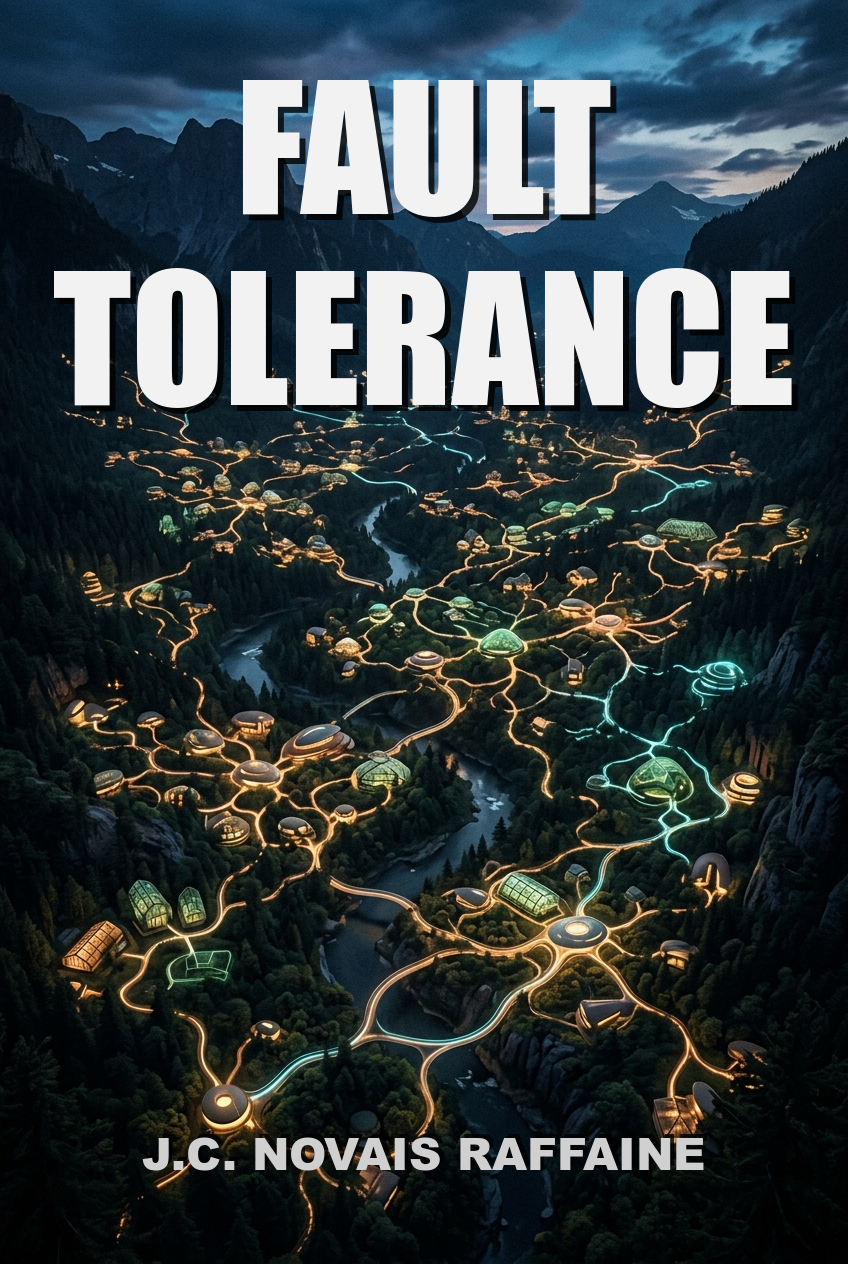
\includepdf[pages={1}, width=\paperwidth, height=\paperheight, keepaspectratio=false]{cover.png}

% --- Copyright Page (Verso) ---
\newpage
\thispagestyle{empty}
\vspace*{\fill}

\begin{flushleft}
    {\headerfont\large\textbf{FAULT TOLERANCE}} \\
    {\headerfont\small A Solarpunk Epic of the Polycentric Bioregional Commonwealth} \\
    \vspace{2ex}
    
    {\small \copyright\ 2026 J.C. NOVAIS RAFFAINE. All rights reserved.} \\
    \vspace{2ex}
    
    {\small This work is licensed under a Creative Commons Attribution-ShareAlike 4.0 International License.} \\
    \vspace{2ex}

    {\footnotesize 
    This is a work of fiction. Names, characters, places, and incidents are products of the author's imagination or are used fictitiously. Any resemblance to actual persons, living or dead, or actual events is entirely coincidental. \\
    \vspace{1ex}
    
    The protocols and technical specifications described herein are released under the Collective Open Source License. For more information, visit: \\
    \headerfont\color{collectiveBlue} github.com/raffaine/collective
    }
    
    \vspace{4ex}
    
    {\headerfont\scriptsize FIRST EDITION} \\
    {\headerfont\scriptsize PRINTED IN THE POLYCENTRIC COMMONWEALTH} \\
    \vspace{2ex}
    
    {\headerfont\tiny 10 9 8 7 6 5 4 3 2 1}
\end{flushleft}
\vspace{2ex}

% --- Title Page (Recto) and TOC ---
\frontmatter

% --- Title Page (Recto) and TOC ---
\frontmatter
\maketitle
\tableofcontents

% --- Main Content ---
\mainmatter

\chapter{The Dream and the Weight}







The morning broke without a siren, without the frantic, artificial urgency of the world outside. For Gabe, dawn was simply a shift in warmth, a gentle gradient of amber light slipping through the wooden shutters, and the soft \textit{click} of the wall heater cycling down as the first rays of sun struck the solar canopy above his cabin. 

He was sixteen now, his limbs long and clumsy with recent growth, but the room accommodated him effortlessly. He stretched, kicking off the heavy cotton quilt. The air inside was crisp and still, hushed by the thick insulation packed into the timber walls. It was a deep, physical quiet, sheltered under the community’s shared promise of peace and stillness. He breathed in deeply, tasting the faint, clean scent of cedar and the morning dew that clung to the outer siding. 

But as Gabe rolled over to check the small e-ink display set into the wooden headboard, his eyes caught the ugly, beige intrusion mounted just outside his window. It was the legacy utility meter, courtesy of the regional power monopoly, Pacific Gas \& Electric. They generated ninety-five percent of their own electricity here, sharing the surplus across the microgrids of the Polycentric Bioregional Commonwealth, storing the rest in massive repurposed battery banks buried beneath the central commons. But the county building code demanded an active grid connection. The meter sat there like a persistent tick on the side of a healthy animal, its digital readout blinking a string of zeroes, a mandated, parasitic tether to the failing systems of the old world. 

Gabe stared at it for a moment, tracing the stark, plastic casing with his eyes. It was a seam in the sanctuary, a reminder that they hadn't actually escaped the world; they were merely floating on top of it, wrapped in bureaucratic camouflage. 

He dressed quickly in a pair of durable hemp trousers and a soft, undyed shirt he’d pulled from the local textile commons the week prior. He grabbed his worn canvas satchel, his fingers brushing against the smooth wood of the door frame. A hidden reader, tucked seamlessly behind the timber grain, recognized the chip in his ring. The deadbolt retracted with a satisfying, heavy \textit{thunk}, welcoming him out into the morning.

Stepping outside, the visual quiet of the settlement hit him. It was a sensation he took for granted, a native reality, but one his mother, Elara, constantly remarked upon with a reverence he couldn't quite fathom. There were no billboards here. No flashing neon demanding his attention, no glaring screens engineered to manufacture anxiety and want. The buildings around him were low, warm, and built to a human scale. Vine-draped trellises arched over the pedestrian pathways, heavy with clusters of kiwi and passionfruit, shading the crushed-granite gravel that drank in the morning dew and fed the underground cisterns. 

He walked down the gentle slope toward the center of the hub, his boots crunching softly. To his left lay the childcare yard, the shared nursery where he had spent his own early years. He paused by the low, cedar-slat fence, resting his forearms on the smoothed wood, letting the morning sun warm his shoulders. 

Inside the shaded yard, a dozen toddlers were already engaged in chaotic, joyful excavation of a massive dirt pile. There were no plastic toys, only wooden blocks, miniature water channels, and glorious, unrestricted mud. A pair of elders sat on a shaded bench under a sprawling oak, weaving baskets from soaked willow branches and keeping a watchful, unhurried eye on the children. The air carried a gentle hum of laughter and discovery, completely free of the harsh fluorescent glare and institutional dread that characterized the daycares of the outside world. 

Yet, bolted to the very fence he leaned against was a stark, legally mandated aluminum sign. Its sharp corners and blocky, authoritarian font clashed violently with the organic curves of the settlement: \textbf{PROPERTY OF GENESIS SOCIAL PURPOSE CORPORATION. LIABILITY LIMITS APPLY. PRIVATE PROPERTY. NO TRESPASSING.}

Gabe traced the raised lettering with his finger, feeling the cold metal. \textit{Genesis Social Purpose Corp}. It was the shell, the legal fiction his mother and the founders had spun to protect this node. To the kids inside, this was the Cultural Commons, a vibrant routing hub in the Polycentric Bioregional Commonwealth. They weren't an isolated experiment; they were networked deeply, exchanging heirloom seed stocks, firmware patches, and mutual aid with the highland hubs to the east and the riverine enclaves down in the delta. To the county tax assessor, the fire marshal, and the zoning board, however, this was merely a corporate retreat facility running a quirky agricultural research project. The sign was the mask they wore to survive the old world's predatory gaze.

A low, mechanical rumble vibrated through the soles of his boots, disrupting the pastoral calm. Gabe looked up toward the main access road that snaked out toward the state highway. An idling diesel engine broke the morning quiet, throwing a plume of acrid gray exhaust into the clean air. It was an old commercial delivery truck with faded corporate logos and dented side panels, coughing out the last breaths of the fossil fuel era. 

The driver, a woman with deep, exhaustion-bruised eyes and a frayed fluorescent safety vest, was scanning a barcode on a heavy, plastic-wrapped pallet. She looked miserable, tethered to a routing algorithm that dictated her every bathroom break, punishing her wages for a suboptimal steering wheel turn or a minute spent idle. She existed in a state of continuous extraction.

Gabe watched as one of the perimeter wardens, a tall man named Silas, approached the truck. Silas was smiling warmly, signing the digital clipboard. He offered the driver a steaming thermos of hot herbal tea and a fresh, warm pastry from the bakehouse. The driver accepted it with a bewildered, grateful nod, her shoulders dropping a fraction of an inch before she climbed back into the noisy cab. 

The delivery was necessary. They could trade cold-hardy wheat and software updates with the highland hubs all day, but they couldn't yet manufacture their own microchips or weave the fine membranes needed for the water filtration plant. They still had to buy things from the dying beast, paying in dollars drawn from their carefully managed reserves. The boundary between the old world and the new was porous, and the price was steep.

His stomach grumbled, pulling him away from the complex layering of their reality. He continued down the path, the smell of wet soil and diesel exhaust giving way to the rich, savory aromas of the Commons Kitchen.

The hearth was the beating heart of the settlement. As Gabe pushed through the heavy, reclaimed-wood swing doors, a wave of comfortable heat washed over him. The kitchen was a cavernous, warmly retrofitted space. Wide electric cooktops hummed quietly without the choking fumes of gas burners. Massive copper pots bubbled with bone broth, and tiers of fresh herbs and greens lined the sunlit far wall.

Fifty people were already gathered at the long, polished oak tables, passing heavy ceramic bowls family-style. The air was thick with the scent of toasted sesame, fermented chili paste, and fresh sourdough. 

"Gabe! Over here!" 

He spotted a few of the other apprentices waving him over from a corner table. Before joining them, he detoured to the warming cubbies along the counter. He tapped his ring against the wooden panel, and a small door clicked open, revealing a heavy stainless-steel lunchbox. The local ledger quietly logged his meal against the hours he had spent in the workshops the day before, with no middlemen, swipe fees, or corporate tracking standing in between. Just warm food shared fairly for honest work, balanced effortlessly across the community's ledger.

He slid into the wooden bench beside his friends, flipping the latches on the tin. Inside was a hearty breakfast: blistered garden tomatoes, a thick slice of sourdough, and a scramble of pasture-raised eggs. 

"Did you hear the perimeter alerts last night?" asked Leo, a younger apprentice, his mouth full of bread. He had rich, dark soil under his fingernails from the morning greenhouse shift. 

Gabe shook his head, scraping his fork against the steel. "No. I was out cold. Once my shutters are closed, I don't hear a thing. Why? Was it coyotes by the fence again?"

"I wish it was coyotes," Leo muttered, his voice dropping below the ambient clatter of dishes and morning laughter. "Something probed the outer municipal firewall. My dad was on the cyber-rotation last night. He said it wasn't a script kiddie or a random botnet. Looked like a coordinated municipal code-enforcement sweep. They were trying to find a gap in our Transient Occupancy tax shielding."

"Transient Occupancy?" Gabe echoed, frowning. "We live here. We aren't transient. I’ve lived in this valley my entire life."

Next to Leo, an older apprentice named Lyra sighed, pushing her glasses up her nose. "Yeah, but Genesis SPC is legally zoned as a short-term agricultural retreat to avoid the county's single-family density restrictions," she explained, her tone dry and precise, parroting the administrative reality she’d learned in the bureaucratic defense seminars. "If the county algorithm detects that we've been residing in the timber cabins for more than two hundred and ninety days consecutively without 'rotating' out to one of the other Commonwealth nodes, the zoning board can legally reclassify us."

"And if they reclassify us?" Gabe asked, suddenly feeling a cold draft that had nothing to do with the ambient temperature.

"They trigger retroactive code compliance for residential subdivisions," Lyra said flatly. "Which means they demand paved roads, grid-tied sewer connections we don't have, and property tax reassessments at suburban development rates. It would bankrupt the settlement in six months."

Gabe felt the idyllic warmth of the kitchen suddenly slip, replaced by a cold, administrative dread. He looked down at his meal. The abundance of their life was real, but it rested on a razor's edge of paperwork, legal loopholes, and relentless camouflage. They were builders, engineers, and farmers, yet their survival depended just as much on bending the county code and finding every possible gap in how the law defined 'occupancy,' 'temporary structures,' and 'agricultural accessory.' 

He chewed his food slowly, the taste of the fresh tomatoes suddenly heavy with the fragility of the soil they grew in. If the legal wrapper tore, the state wouldn't send tanks or riot police first; they would send building inspectors, tax liens, and foreclosure notices. The sanctuary wouldn't burn; it would simply be drowned in paperwork and legally seized by a bank.

\textit{ } *

A mile away, in the subterranean cooling hum of the central routing hub, Elara felt the phantom weight of the old world pressing against her temples, threatening to crush her skull.

She stared at the wall of monitors, the living map of the settlement pulsing in quiet waves across the screens. She was forty-two now, the silver threads in her dark hair a physical ledger of the immense stress it took to pull this community from the ashes of the legacy system and keep it breathing in tandem with the rest of the Commonwealth. 

The room was bathed in the pale blue light of the terminals. Unlike the organic, sunlit world Gabe was walking through above, this space was industrial, watchful, and intensely pragmatic. The air was kept at a brisk sixty-five degrees to keep the servers from overheating. It was the nerve center of their legal and financial defense, the quiet battlefield where the survival of their valley was negotiated, compromised, and fought for every single day. 

To the people outside, the law was just the air they breathed. For Elara, the old world's taxes, zoning boards, and commercial banks formed a hostile border she had to patrol every waking hour. 

Unlike Gabe, Elara remembered the Before in vivid, suffocating detail. She remembered the specific, grinding exhaustion of the day Gabe was two years old and had a raging ear infection. She remembered sitting in her car in the parking lot of a corporate-owned urgent care clinic, crying in frustration as she navigated a Kafkaesque insurance portal on her phone, knowing that walking through those sliding glass doors would cost her half her month's rent. 

She remembered Kael, her old mentor, finding her in that desolate era. Kael had seen the structural collapse coming decades out, quietly laying the philosophical groundwork for the Polycentric Bioregional Commonwealth. It was Kael who had offered her the door out of the maze, teaching her the principles of resilient localism. And it was Jax, the brilliant, perpetually abrasive architect, who had provided the technical element. Jax had written the mesh protocols that now seamlessly linked the highland hubs to the coastal nodes, entirely bypassing the corporate internet backbone. 

Kael had given them the dream and Jax had built the network, leaving Elara to carry the daily weight of keeping their pocket of the future safe from the dying past.

She and the founders had built this shield so the kids wouldn't ever have to know that terror. But building a refuge and keeping it standing were two very different things. The youth thought their protection was the mesh network, the solar canopy, and the mutual aid economy. They thought it was simply about being a self-reliant node in the Commonwealth. 

But they weren't entirely free. Nobody was allowed to be truly free anymore. The legacy system didn't permit vacuums; it viewed autonomy as a threat to its revenue streams.

The real shield was the administrative facade. It was the fact that Elara spent four hours a day acting as the Chief Operating Officer of \textit{Genesis Social Purpose Corporation}. It was the exhausting, continuous performance of pretending to be a failing, slightly eccentric capitalist enterprise. 

On the screen to her left, a legacy banking portal sat open, its outdated, clunky interface a jarring contrast to the clean, local ledgers running on her main display. Elara watched with a familiar, sickening tightness in her chest as the progress bar loaded. She was putting through a wire transfer, converting tens of thousands of their hard-earned community credits through a chain of quiet exchanges into ordinary dollars just to pay the county's steep quarterly property taxes. 

\textit{Transaction Approved. Funds Transferred.}

The money vanished into the state's coffers. It was extortion, pure and simple. A bribe paid to the dying empire to look the other way for another ninety days. If they missed a payment, the county would send the sheriff to seize the land, auctioning their rich permaculture soil and timber workshops to the highest corporate bidder to be bulldozed for a logistics warehouse. 

"Elara," a voice crackled over the wired radio channel, pulling her from her dark reverie. It was Marcus, one of the perimeter wardens, calling from the outer watchtower. "Are you seeing this activity on the outer gate?"

Elara minimized the banking portal, pulling the security log to the center screen. Her fingers flew across the keyboard, her posture instantly shifting from bureaucratic fatigue to sharp focus. 

"I see it," she said, her voice dropping an octave. "It’s not just a routine check. They’re trying to fake a member credential to get inside our records."

"County?" Marcus asked, the static popping lightly. 

"Looks like it," she said, her eyes tracking lines of logs scrolling rapidly in the terminal. "County Assessor's office, probably routed through a private audit firm. They’re getting desperate. It’s not just drones scanning for unpermitted structures from the sky anymore. We disguised the compost digesters to look like standard grain silos, and that threw them off. Now they're trying to slip a fake inspection key into our housing records to prove we have permanent residents."

A brief cluster of red markers flared across the screen as the outer gateway blocked another intrusion. 

Elara slumped back in her chair, rubbing her eyes with the heels of her hands. The server room smelled of warm dust, hot metal, and stale coffee. It was the smell of friction. She knew better than anyone how well the settlement was thriving. She saw the harvest numbers, the sheer volume of rich, black organic compost generated, the logs showing seamless resource sharing with the riverine enclaves. She knew Gabe was probably sitting in the communal kitchen right now, eating food grown entirely outside the corporate supply chain, laughing with friends who weren't crippled by student debt or constant financial dread.

But the beast outside was starving. The legacy economy was collapsing under its own extractive weight. Commercial real estate was vacant, the municipal tax base was evaporating, and city bond yields were plummeting. And as the city starved, it looked hungrily at the thriving, independent nodes of the Commonwealth. 

The authorities didn't see an ecological sanctuary; they saw an untapped, rogue revenue stream. They saw networks of people living, working, and sharing without generating sales tax, without paying income tax on their internal labor exchange, and without relying on corporate utilities. To the hungry calculators at City Hall, the Commonwealth was a massive tax-evasion scheme hiding behind agricultural zoning variances.

A soft chime interrupted her thoughts. A message from the weather station in the coppice woods. The temperature was dropping fast, an unseasonal chill rolling in from the coast. 

\textit{Wear and tear,} she thought, closing her eyes for a brief second. \textit{It never stops. You build a garden, and the weeds try to swallow it. You build a sanctuary, and the state tries to tax it.}

She opened a secure window and began typing a rapid sequence of commands to tighten the gateway rules. She couldn't simply block the county's audit firm outright, since a hard block would raise an immediate red flag and bring armed deputies to the gate with an inspection warrant. Instead, she had to feed them fabricated, perfectly ordinary records. She diverted their probe into a decoy directory, feeding it a neat, fictional set of paperwork that confirmed Genesis SPC’s compliance: \textit{Yes, occupancy is below the legal threshold. No, the cabins are not permanent homes; they are temporary seasonal worker housing. Yes, water usage matches standard orchard irrigation.} 

It was a delicate, high-stakes game of digital sleight of hand. She was maintaining a complete, real-time paper trail of a boring corporate farm just to keep the hounds at bay. 

"I've patched the gate, Marcus," she said into the mic, her voice steady and calm, betraying none of the bone-deep exhaustion she felt. "I fed them the decoy records. That should keep their audit software happy for now. But keep your eyes on the road. If they aren't finding what they want in the files, they'll send someone in person. They might send an inspector to look for a cracked pipe, a frayed wire, or an unpermitted shed. We can't give them a single excuse to step past the gate."

"Copy that," Marcus replied. "Wardens are on high alert. We'll run a visual sweep of the exterior conduit lines just to be sure. I'll make sure the 'Agricultural Use Only' signs are clearly visible on the timber cabins and the schoolhouse before the morning shift starts."

Elara terminated the connection and stood up, her joints popping in the cool, dehumidified air of the server room. She looked back at the screens one last time, watching the green pulse of their internal systems overlaid with the red, aggressive pings of the outside world. 

The utopian dream of the Commonwealth was beautiful, but it wasn't magic. It was a machine. A machine made of people, of trust, of endless, grinding maintenance. It was held together by legal duct tape, shadow economics, and the sheer willpower of the adults who stood on the boundary line, facing outward into the storm so the children could face inward toward the sun.

And right now, she could hear the ticking of a clock that Gabe, in his beautiful, shielded innocence, was only just beginning to perceive. The old world wasn't done with them. Not by a long shot. They could build the highest walls, write the most elegant code, and cultivate the richest soil, but as long as they existed on the same physical planet as the legacy system, they were bound to its decaying, desperate gravity.

She grabbed her heavy wool coat from the back of her chair. The thick wool carried the faint, comforting smell of woodsmoke from the biochar kilns, grounding her in the physical reality of what they were building. She strapped her portable terminal to her wrist, checking the battery charge, and headed toward the heavy steel blast door that led to the surface. 

It was time to pay the piper. It was time to walk the perimeter, smile at the delivery drivers, placate the county inspectors, and ensure the legal fiction was perfectly intact. The weight of the administrative camouflage was crushing, but as she thought of Gabe walking freely under the solar canopy, breathing clean air, she squared her shoulders. It was a weight she would carry until it broke her, or until the old world finally crumbled to dust.

\chapter{Genesis}

The perimeter of the local node was not a wall. Walls were legacy architecture, brittle and authoritarian, demanding constant armed defense. The perimeter was a living boundary of crushed gravel, dense blackberry brambles, and small cameras tucked into the canopy of the oak trees. It breathed, it filtered, and today, it was choking on the exhaust of the old world. This sanctuary was merely one cell in the sprawling Polycentric Bioregional Commonwealth, a vast network of mutual aid that stretched across the fractured continent.

Elara stood at the edge of the access road, the afternoon sun beating down on her shoulders, the heat radiating off the cracked asphalt in shimmering waves. The air tasted of hot tar and diesel exhaust, a bitter contrast to the cool, cedar-scented shade of the interior hubs. Beside her, Marcus held a pair of heavy, grease-stained binoculars, his jaw tight. 

"Five of them," Marcus muttered, lowering the glasses. "A family, maybe, or neighbors who stuck together. They look like they walked the last ten miles from the state highway. Their car is dead on the shoulder."

Elara adjusted the heavy canvas strap of her satchel, feeling the reassuring weight of the onboarding kit resting against her hip. "Did the lookouts spot any county cruisers following them?"

"None," Marcus said, wiping sweat from his forehead with the back of a dirt-caked glove. "No county drones overhead. No patrol cars. Just them. And they look completely spent. The neighboring nodes sent word they might be heading our way."

As the group crested the gentle rise of the access road, the physical toll of their journey became undeniable. They were dragging their lives in bursting duffel bags and a rusted, rattling utility wagon. The man at the front had the hollow, hunted look of someone who had been chewed up by app-dispatched gig work until his bones showed. His shoes were taped together. A woman walked beside him, clutching a sleeping toddler to her chest, her eyes darting frantically across the tree line, expecting the surveillance cameras that lined every street in the city. Two teenagers trailed behind, their heads down, shoulders hunched against the weight of a society that had already discarded them.

They had reached the outer threshold, the quiet border where the wreckage of the collapsing state met the living ground of the Commonwealth. 

Elara stepped forward, her boots crunching loudly on the gravel, deliberately breaking the tense silence. She didn't carry a weapon; she carried a clipboard and a heavy thermos of cold, mineral-rich water drawn from the deep well. 

"Stop there, please," Elara said. Her voice was calm but carried the quiet authority of the boundary. 

The man flinched, dropping the handle of the wagon. It hit the dirt with a heavy thud. He immediately reached into his pocket, his hands shaking, and pulled out a cracked smartphone and a plastic wallet. "We have the forms," he stammered, his voice dry and reedy. "I have my credit score, it's not great, but I can work. I have my background check from the county. We just need... we just need a place to stay. A lease. Anything."

He was offering his neck to the collar. It was the only way he knew how to survive: hand over his records, prove he was profitable, and beg for the privilege of being worked to the bone.

"Put that away," Elara said softly, closing the distance between them. She unscrewed the cup of the thermos, filled it with the cold water, and handed it to the woman holding the child. "We don't use credit scores here. We don't care about the county's background checks. Drink this. Then we figure out how you fit in."

The woman took the cup with trembling hands, drinking greedily, the water spilling down her dusty chin. The toddler stirred, letting out a weak, thirsty whimper. 

Elara looked at the man's hands. They were calloused, stained with motor oil and deep grease that never quite washed out. "What do you do?" she asked.

"I'm a mechanic," he said, swallowing hard. "Small engines. Pumps. I fix things. My wife, Sarah... she's a seamstress. Industrial machines."

Elara felt a sudden surge of relief. \textit{Metric wrenches and an industrial sewing machine.} They weren't just mouths to feed; they were skilled hands bringing fresh strength into the community. But the transition wouldn't be easy. 

"My name is Elara," she said, tapping the small screen on her wrist. A green light blinked, quietly logging their arrival with the settlement's records. "You're off the grid now. Which means the rules have changed. We don't do leases, and we don't do debt. But to come inside, you have to leave the ghosts of the old world at this line."

She pulled a rugged weatherproof case from her bag and popped the latches, revealing a compact offline circuit board and a pair of keycard writers. As she opened it, the man stared at the electronics as if she had pulled out a bomb. 

"What is that?" he asked, backing up a half-step. "Is that a scanner? I told you, I have my ID—"

"It's just a key maker," Elara interrupted, her tone firm but gentle. "To live and work here, you need a local keycard. It doesn't connect to the internet. It doesn't report to corporate dispatchers or the authorities. It stays here, on our own wires, linking only to our sister communities. But I can't just hand you the keys to the workshops. Trust here isn't assumed, and it isn't bought. It's built. In person."

Looking at the terrified, exhausted faces of the newcomers, a wave of dizziness washed over Elara. The smell of the hot dust and the sight of the blinking green light on her wrist threw her backward in time. She wasn't standing on the gravel road in the present; she was standing in the mud seven years ago, in the pouring rain of their first winter.

\textit{}*

\textit{The memory tasted of copper and ash.}

\textit{It was Year Zero. The settlement was nothing more than a desperate manifesto, fifty terrified people, and an abandoned industrial lot they had secured through a tangled commercial lease. They called that first winter the System Call, when they tried for the first time to run a brand-new society on real, messy human beings.}

\textit{It had nearly killed them.}

\textit{Elara remembered the relentless, freezing rain of that first November. They had tried to run the community entirely by software rules. Jax, their brilliant but stubborn technical architect, had designed what he thought was a flawless automated system. Every chore and ration was tracked on a digital ledger. Every rule was enforced by code. Jax believed that if the math was fair, people would naturally get along.}

\textit{He was wrong. Math doesn't bleed, and it doesn't get cold.}

\textit{Elara remembered kneeling in the mud outside the half-built kitchen, her hands numb, trying to splice a severed data cable while Jax frantically tried to keep the system from crashing. A bitter fight had broken out over the heavy winter blankets. The automated heating program had a flaw, diverting power to keep the computer servers cool instead of warming the nursery where the children slept.}

\textit{A man named Jonas, pushed to the brink of freezing and panic, had taken a crowbar to the main server rack, screaming that the computer was starving them. Their elegant digital system had shattered the first time it met real physical hardship.}

\textit{They had learned, the hard way, that no computer program can replace human trust. Their rules had been completely disconnected from the reality of survival. The code was suffocating the people it was meant to serve.}

\textit{That night, shivering around a fire in a rusted oil drum, Elara and the remaining founders had rewritten the rules from scratch. They threw out Jax's purely automated governance and built the Kinship Protocol. They realized that drawing from the food stores, running heavy machinery, or making decisions that affected everyone's safety could never be left to a faceless keycard alone. Every card had to be backed by a real human bond.}

\textit{They had held their first Vouching Circle that very night. It wasn't a digital form; it was a promise made face-to-face. They forced themselves to look each other in the eyes. It was Kael, her mentor, who stepped forward first. Kael looked past the anger and fear, ladling out the last of their hot rice and beans, handing Elara a warm bowl in the rain, and standing up to vouch for her. Under the new rule, if Jonas took a crowbar to the equipment again, the people who had vouched for him would lose their own workshop privileges right alongside him. Responsibility became personal, shared, and real.}

\textit{They learned that a community couldn't live on a screen; it had to be rooted in the soil. It had to smell like sweat and woodsmoke. That was the hard-won lesson of their founding: a free society needs human closeness to create warmth.}

\textit{}*

The sharp click of the case snapping shut brought Elara back to the present. 

The mechanic, who had introduced himself as David, was staring at her, waiting. 

"We need your phones," Elara said, holding out a heavy, signal-blocking pouch. "Smartphones, smartwatches, anything with a cell signal. The county tracks phone signals to estimate how many people are living out here. If you carry those past the gate, you light us up on their map."

David hesitated, his thumb hovering over the cracked screen of his phone. It was his last tether to the only world he knew, a familiar misery of debt collectors and app dispatchers. Slowly, he dropped it into the pouch. Sarah followed, adding her phone. The teenagers surrendered theirs with reluctant, wary glances.

"Good," Elara said, sealing the pouch and setting it in the back of her electric utility cart. "Now, let's log what you brought. Marcus?"

Marcus stepped forward with a handheld scanner. He didn't point it at the people; he pointed it at their wagon, logging the heavy, oil-stained toolbox. 
 
"Metric tool set," Marcus read from his pad. "We'll set that up in the main repair shop."

He tagged the bulky, canvas-wrapped shape in the back of the wagon. "Industrial sewing machine. Headed for the textile workshop."

Elara watched David's face closely. "You're bringing real tools and real skills into the community," she explained plainly. "That means you aren't starting from scratch. We're setting your family up with a full share of power and supplies right away."

"A what?" David asked, wiping his mouth. "A loan? What's the interest rate? Because if it's like the payday places—"

"There is no interest rate," Elara said firmly, cutting through his fear. "There is no money inside this fence. We're giving you a share of our electricity, our food, and a roof over your head. As you settle in and set up your tools, fix pumps, or help in the kitchen, you contribute back to the commons. You work, you eat, you live. Nobody is skimming profit off your back. And when our valley produces more than we need, we share the surplus with our sister communities."

She tapped her wrist screen, sending a welcome notice ahead to the settlement. Down in the valley, the housing stewards' board updated, marking a family cabin ready. 

"We've set aside a place for you," Elara continued, gesturing toward the interior of the settlement. "It's a family cabin with an attached workspace. It has beds, a heater, and a lock on the door. As of right now, it's yours."

They loaded the exhausted family into the electric cart, the quiet hum of the motor carrying them past the perimeter and into the heart of the valley. 

As they rode, the rigid tension in the newcomers visibly began to melt, replaced by a quiet wonder. They passed the coppice woods, where workers were harvesting fast-growing willow poles, the air smelling sharply of cut green wood and rich compost. They passed the cabins, their solar roofs glinting in the late afternoon sun. 

David stared at the people walking the paths. They were dirty, sweating, and carrying loads of lumber and garden greens, but their faces were free of the frantic, hunted exhaustion he knew so well. There were no billboards. There were no sirens. 

The cart rolled to a stop outside the wide, open-air pavilion of the Commons Kitchen. The smells of roasting garlic, wood-fired bread, and rich, simmering broth hit the newcomers all at once. The toddler began to cry again, this time from pure hunger.

"This is the Hearth," Elara said, stepping out of the cart. "This is the heart of our home."

Inside, the evening meal was coming together. Wide electric stoves hummed softly. Dozens of people were chopping vegetables, stirring pots, and laughing. In the center of the hall sat a massive, polished oak table. Set flush into the center of the wood was a small brass-rimmed reader known as the Hearth Table Anchor.

"We've logged your tools, and we've given you a home," Elara said, turning to David and Sarah. "Food and shelter are yours no matter what. But before you can run the heavy machinery in the workshops or draw heavy power from the grid, you have to be welcomed into the community's trust. You need someone here to vouch for you."

"A background check," David said, his shoulders slumping instinctively. "Look, my credit is shot. I had a dispute with a landlord, they put an eviction on my record—"

"I told you to leave those ghosts at the gate," Elara said, her voice softening with the deep empathy of someone who had stood in his shoes. "We don't care about landlords or credit bureaus here."

She pulled out two blank wooden-inlaid keycards and handed one to David and one to Sarah.

"Out there, survival is held hostage," Elara explained, resting her hand on the heavy oak table. "They use the threat of hunger and homelessness to keep you obedient. If you lose your job, you lose your roof. Here, your basic needs are never on the line. You will always eat. You will always have a warm bed. You could argue with every neighbor in this valley, and you would still get a hot bowl of soup every night."

Sarah let out a long, shaky breath, holding her child close. 

"But," Elara continued, her gaze steady, "you want to work in the metal shop and the heavy repair bays. Those machines use a lot of power, and they can hurt people if they're misused. To unlock those doors, you need a neighbor to stake their own good name on yours."

"Who would do that?" David asked, looking around at the strangers in the kitchen. "Nobody knows us."

"I will," Elara said simply.

Marcus, who had just walked in carrying a crate of tomatoes, stopped in his tracks. "Elara, wait. You're our lead steward. You carry more responsibility than anyone here. If they trash a workshop or hurt someone, it comes straight back on you. You'd lose your own clearance to manage the valley's records."

"I know what it means, Marcus," Elara said, never breaking eye contact with David. "If they let us down, I answer for it."

She looked from David to Sarah. "This is what real trust looks like. It isn't a signature on a lease. When I vouch for you, my good name is tied to yours. If you steal from these workshops, or if you hurt someone here, the community holds me accountable right alongside you, because I stood up and brought you into our home."

David stared at the card in his hand, feeling the weight of her words settle onto his tired shoulders. This wasn't a fine print contract; it was a human being placing herself in his hands. This woman, a stranger ten minutes ago, was trusting him with her own standing in the community, purely because of the calluses on his hands and the honesty in his voice.

"Why?" David whispered. 

"Because ten years ago, someone did it for me," Elara said, remembering Kael in the pouring rain, handing her a warm bowl of rice and beans when she had nothing left. 

She tapped the reader set into the oak table, waking the small screen. 

"Lay your cards on the wood," she said gently. 

David and Sarah stepped forward. The chatter around the nearby prep tables quieted as several neighbors paused their chopping to watch. It was a familiar, cherished moment in the hall. 

Elara rested her scarred wooden ring against the brass rim of the reader. David and Sarah laid their new cards beside her hand. 

The reader glowed a warm blue. Down in the server room, the local network recorded the new bond and shared it with the neighboring valleys. Because their hands were resting at the very same table at the very same moment, the community ledger knew this wasn't an anonymous click from miles away, but neighbors standing side by side and looking each other in the eye. The bond was sealed. 

But the welcome wasn't finished. 

Elara reached across the oak table and took a heavy ceramic bowl from the stack. She ladled it full of thick, steaming broth and handed it to David. She filled another for Sarah and the children, and finally one for herself. 

"The ledger only needs us standing at the same table," Elara said, picking up a wooden spoon. "People need to break bread. Sit down and eat."

David took a spoonful of the stew. It was rich, savory, and real. The constant, gnawing dread of the outside world began to loosen its grip on his chest, replaced by the simple warmth of a shared meal. He looked at Elara, his eyes bright with unshed tears, and gave a quiet nod.

On Elara's wrist screen, a soft chime confirmed the update. Their cabin was warm, the workshop doors would open to their hands in the morning, and their names were woven into the life of the valley.

The community had grown. The circle was a little wider, the shared hands a little stronger. Elara felt the familiar weight of the promise she had just made, a quiet responsibility she would carry until the family found their footing. 

But as she watched the exhausted parents finally sit down and eat, their toddler smiling over a piece of warm bread amid the warmth and laughter of the hall, she knew the risk was worth every bit of it. They had pulled one more family out of the wreckage outside and brought them home.

And tomorrow, the real work would begin.

\chapter{Friction and Threads}

\epigraph{They measured the seams of the failing state, \\
And patched the fraying edges of the perimeter gate. \\
Every stitch in the canvas, every line of the code, \\
Is a heavy thermodynamic debt we are owed.}{The Coppice Chorus, "Sashiko Protocols" (Recorded in the Lambda Cultural Commons)}

The heavy, rhythmic \textit{thud-thud-thud} of the walking-foot sewing machine vibrated through the dense oak floorboards of the Nu Textile Commons. The room was a cavern of focused, kinetic energy, smelling intensely of hot machine oil, damp wool, and the sharp, metallic tang of iron mordant from the botanical dye vats bubbling in the corner. The air was thick, carrying the undeniable, physical weight of labor. It was a space designed not for consumption, but for the relentless war against entropy.

Silas sat hunched over a wide, scarred wooden cutting table near the center of the room. His broad shoulders, usually relaxed in the open air of the perimeter patrols, were tense with concentration. He was driving a heavy steel bodkin through the thick, resistant collar of a canvas work jacket. He employed a visible Sashiko mending technique, pulling thick, white bast-fiber thread through the indigo-dyed fabric in tight, geometric patterns. He was reinforcing the abrasion points where the heavy timber chains of the coppice crews inevitably bit into the shoulders of the haulers. 

In the legacy world—the suffocating reality that sprawled just beyond their carefully maintained boundaries—this jacket would have been tossed into a landfill the moment the collar frayed. It would have been instantly replaced by a cheap, petrochemical-derived synthetic garment engineered to fail, designed to shed microplastics into the municipal watershed with every wash. But here, within the Collective, clothing was not a disposable commodity. It was soft infrastructure. 

By patching the canvas, Silas was executing a physical, thermodynamic mandate. The mending process restored the garment's structural integrity while consuming less than fifteen percent of the exergy required for virgin fabrication. It was a tangible victory, a small but fiercely held perimeter against the culture of infinite extraction.

Elara pushed through the heavy wooden doors, the ambient noise of the commons washing over her. The digital paranoia of Layer 7—the proxy servers, the municipal firewalls, the legal camouflage—clung to her like a second skin. She looked exhausted. The bureaucratic weight of maintaining their Genesis Social Purpose Corporation shell was pulling at the corners of her eyes. She carried her heavy canvas satchel, the strap digging into her shoulder.

Silas looked up at the sound of the door. The intense focus on his face broke into a warm, immediate smile that smoothed out the tired lines around his mouth. He set the bodkin down, his large hands resting on the patched canvas.

"You look like you've been arguing with the ghost of a city planner all morning," Silas said, his voice a deep, resonant rumble that effortlessly cut through the mechanical clatter of the room.

Elara offered a tired, half-smile, crossing the room to stand beside his table. The heat radiating from the steam irons and dye vats was comforting, unthawing the chill of the server room that had settled deep in her bones. "Close. I was manually validating the cryptographic ledgers for the county property tax assessment. They changed the API endpoint without notice, hoping we'd default and trigger an automated lien."

Silas shook his head, his fingers tracing the white thread of his handiwork. "The beast is always hungry."

"It's starving," Elara corrected, her eyes dropping to the jacket. "Beautiful work. Who is that for?"

"Marcus," Silas replied. "He tore it up hauling the new perimeter fencing. The structural integrity is back to nominal. It'll cost him a fraction of his thermodynamic value tokens, but he won't have to break in a new rig."

"The newcomers from yesterday," Elara said, shifting her weight. "David and Sarah. They brought a metric toolset and an industrial serger. I routed the serger down here. Has it been integrated?"

"It has," a voice called out from the scrap-sorting hoppers. 

Riya walked over, wiping grease from her hands onto a coarse linen rag. She was tall, with sharp features and hair pulled back into a tight, practical knot. She was a master tailor, a steward of the textile node. She was also Silas's former partner. They had shared a micro-lodging pod for three years before the emotional geometry of their relationship had naturally, gracefully shifted. 

In the legacy world, Elara knew, this interaction would have been fraught with a conditioned, artificial scarcity. The old world demanded nuclear isolation; it engineered jealousy to sell the myth of proprietary love, treating human affection like an exclusive real estate contract. But the Collective had burned those toxic boundaries away. The emotional ledger here didn't operate on zero-sum mechanics. Love and intimacy were a mesh network—resilient, fault-tolerant, and entirely lacking the fragile single points of failure that defined the old world's possessive despair.

Riya placed a warm, familiar hand on Silas's shoulder, leaning in to inspect the Sashiko stitching. "Your tension is a little tight on the left clavicle," she murmured, before turning a bright, genuine smile toward Elara. "We calibrated the serger this morning, Elara. Sarah is resting, but she's already eager to log hours. She knows her way around the machine. We're running all the organic off-cuts into the Mu biochar bins, and she's sorting the synthetics for the Alpha extrusion hoppers."

"Good," Elara said, feeling a knot in her chest loosen. "We need them integrated fast. The faster they are physically grounded in the work, the faster the legacy trauma starts to fade."

Riya squeezed Silas's shoulder gently and stepped back. "I'm going to check the dye vats. The iron mordant is getting temperamental." 

As she walked away, Silas turned his full attention back to Elara. The space between them felt charged, a quiet, magnetic pull that had been steadily growing over the past few months. It wasn't the frantic, desperate clinging of the old world; it was a slow, deliberate gravity. 

"You need to step away from the terminal," Silas said softly. "Your eyes are glassy. Come with me to Alpha. I need to print a replacement mounting bracket for the western perimeter sensor array, and you need to breathe air that hasn't been recycled through a server rack."

Elara hesitated, the phantom weight of her administrative duties pressing down on her. But looking at Silas—at the calloused steadiness of his hands and the quiet grounding of his presence—she nodded. "Okay. A walk. A short one."

\textit{}*

The transition from the Nu Textile Commons to the Alpha Fabrication hub was a shift in both atmosphere and epoch. They left behind the damp, organic smell of natural fibers and stepped into a world of sharp, dry ozone and the distinct, sweet tang of hot PETG filament.

The Fabrication Commons was housed in a retrofitted industrial garage. It was a temple of localized manufacturing, a direct physical refutation of globalized supply chains. Banks of 3D printers, housed in actively heated desiccant dry boxes to protect the filament from moisture, hummed with precise, robotic intent. In the back, a CNC metal router was carving a custom aluminum gear, bathed in a milky stream of cooling fluid. 

There were no centralized servers here. The printers ran on local firmware, communicating entirely via the air-gapped internal mesh network. It was autarky made manifest.

Silas walked over to an available FDM printer, wiping the heated glass bed with an isopropyl-soaked rag. He pulled a digital file from his wrist terminal, holding it up to the optical reader on the printer's edge node. The node chimed, cross-referencing his Verifiable Credential against the system's ledger. 

"Authenticating the print geometry," Silas muttered, his eyes tracking the small e-ink display. "Escrowing the thermodynamic fee. Material cost, electrical draw, and machine wear... locked."

The printer shuddered to life, the stepper motors engaging with a high-pitched, musical whine. The hotend began to heat, the temperature climbing rapidly toward two hundred and forty degrees Celsius. 

Elara stood beside him, watching the mechanical precision. The heat radiating from the printer bed washed over her. She leaned slightly against Silas, their shoulders brushing. He didn't pull away; instead, he shifted his stance to accommodate her weight, a silent, physical affirmation of their connection.

"It's incredible," Elara said softly, watching the extruder lay down the first, perfectly squished layer of plastic. "In the old world, if that sensor bracket broke, we would have had to order a proprietary piece of injection-molded plastic from a warehouse a thousand miles away. It would have arrived in three days, wrapped in single-use plastic, delivered by an exhausted gig worker. And here... we just summon it from the dirt."

"We don't summon it," Silas corrected gently, his eyes on the print head. "We synthesize it. It still costs energy. It still creates friction. But the friction is local. It's manageable. We aren't outsourcing the entropy to someone else's backyard."

He turned his head to look at her, his expression serious. "You carry too much of the invisible friction, Elara. The proxy wars. The legal defense. We see you slowly grinding down under the weight of Layer 7. You have to let us carry some of it."

Elara looked down at the concrete floor. "You can't carry it, Silas. Not this part. You maintain the physical perimeter. You build the soil, you fix the machines. But if the Ablative Shield fails—if the legal fiction we've built shatters—the state won't care about our thermodynamic efficiency. They'll just send the sheriffs. They'll rezone us, tax us into oblivion, and foreclose on the land. I have to stand in that doorway."

"You don't have to stand there alone," he said, reaching out to touch her arm. His fingers were rough, but his touch was incredibly gentle. 

Before Elara could respond, a violent, high-frequency vibration shuddered up her arm. Her wrist terminal was flashing a blinding, angry crimson. The ambient, low-level hum of the digital twin had suddenly spiked into a deafening roar of algorithmic alarm. 

Silas stiffened, his hand dropping from her arm. "What is it?"

Elara was already swiping frantically at the small screen, pulling up the diagnostic telemetry. Her heart hammered a frantic rhythm against her ribs. The romantic gravity of a moment before was instantly obliterated by cold, adrenalized terror.

"It's a Layer 7 breach attempt," Elara said, her voice tight, the words clipping sharply. "Municipal probe. But it's not a standard automated ping. It's an aggressive, directed code compliance sweep."

"Where?" Silas demanded, his posture shifting instantly from maker to warden. 

"They're hitting the external proxy," Elara said, her eyes tracking the cascading logs. "The county tax assessor's algorithms. They're trying to bypass the Genesis SPC firewall and query our raw acoustic and thermal telemetry directly."

Silas swore under his breath. "They're looking for the foundries. They're looking for the fabrication commons."

"Exactly," Elara said, her fingers flying over the virtual keyboard. "If they capture the thermal signature of this room, or the electrical draw of the CNC routers, they can prove we aren't an agricultural facility. They'll reclassify the entire settlement as an unpermitted industrial manufacturing zone. The fines alone would bankrupt us by Tuesday."

The threat wasn't abstract anymore. It wasn't a slow, creeping entropy. It was an active, hostile hunter, probing their defenses for a weak point, eager to devour their autarky and feed it to the starving legacy grid.

"What do we do?" Silas asked, already moving toward the heavy rolling door of the garage. 

"I need to execute a causal rollback on the external-facing ledger," Elara said, her mind racing through the defensive protocols of the Adversarial Mesh. "I have to feed them a spoofed, benign state. I have to make this room look like a temperature-controlled greenhouse to their sensors."

"And physically?" 

"Physically, you need to lock down the perimeter!" Elara shouted, looking up from the terminal. "If they don't get the data digitally, they might deploy a low-altitude municipal drone to scan for thermal venting. Shut the bay doors. Kill the exhaust fans. Cut power to the CNC router immediately. We have to go perfectly cold from the outside."

Silas didn't hesitate. He sprinted across the shop floor. He hit the emergency stop on the CNC router, the heavy machine spinning down with a dying groan. He grabbed the heavy steel chains of the rolling bay doors and hauled them down, the metal crashing against the concrete floor, plunging the room into the dim, artificial light of the emergency LEDs. 

The heat in the room immediately began to climb, the thermal exhaust trapped inside the cinderblock walls. It was suffocating.

Elara dropped to her knees right there on the concrete, pulling a secure, hardened tablet from her satchel. She connected a physical cable from the tablet directly into the network switch mounted on the wall, bypassing the wireless layer entirely.

She was sweating, the heat of the printers and the trapped air making it hard to breathe. \textit{This is the friction,} she thought violently. \textit{This is the cost.}

She dove into the terminal. The municipal algorithms were relentless, hammering against the outer policy gates. They were exploiting a vulnerability in the county's own updated API structure, using it as a wedge to pry open the Transient Occupancy logs. 

Elara established a honeypot—a fake, parallel digital twin of the Fabrication Commons. She routed the incoming queries into the trap, feeding them carefully constructed, mathematically consistent lies. She linked the power draw of the printers to a fabricated log of high-intensity agricultural grow lights. She masked the acoustic vibration of the CNC router as a heavy-duty compost aerator. 

It was a terrifying, high-wire act of cryptographic perjury. If the thermodynamic math didn't balance—if the electrical draw she reported didn't match the ambient thermal bleed—the algorithm would flag the discrepancy and issue a subpoena.

"Hold... hold..." Elara whispered, her thumbs blurring across the screen. The heat in the room was immense now. She could hear Silas pacing near the door, his hand resting on the hilt of his heavy utility knife, listening for the whine of a drone rotor outside. 

The terminal flashed. The external queries spiked, hovering for a long, agonizing second of computational judgment. 

Then, the red text on her screen faded to a cool, neutral gray. 

\textit{Connection Terminated. Audit Status: Compliant. No Violations Found.}

Elara collapsed backward, her shoulders hitting the concrete floor. She let out a long, shuddering breath, staring up at the acoustic tiles of the ceiling. The silence in the room was absolute, save for the persistent, oblivious whir of the 3D printer, still laying down its perfect layer of PETG, indifferent to the war that had just been fought for its existence.

Silas walked over slowly. The heat was oppressive, his shirt dark with sweat. He looked down at her, his expression a mix of profound relief and grim realization. 

"Did we hold the line?" he asked quietly.

"We held it," Elara rasped, closing her eyes. "They bought the proxy data. They think we're just growing very expensive tomatoes."

Silas reached down, offering his hand. Elara took it, letting him pull her up. His grip was strong, an anchor in the storm. 

"It's getting worse," Silas said, looking at the hardened tablet in her hand. "They're getting smarter. More aggressive."

"The legacy system is starving," Elara repeated, the reality of it settling over her like a shroud. "They have no municipal tax base left. Vain's algorithms are strip-mining the suburbs, and now they are looking at us. We are a pocket of density, of wealth, of negentropy. We're a battery they desperately want to plug into."

She looked at Silas, the romantic tension from earlier hardened into something sharper, more resilient. The utopian dream was beautiful, but it was mortgaged against the predatory gravity of the old world. 

"The clock is ticking, Silas," Elara said, her voice barely above a whisper. "The Ablative Shield isn't going to hold forever. The friction is too high. Eventually, we're going to have to decide between staying here and fighting them in the dirt... or cutting the threads completely."

Silas didn't answer. He just tightened his grip on her hand, looking toward the sealed metal door, listening to the heavy silence of the world outside.

\chapter{Nourishing the Resistance}











The heat was a physical wall, a shimmering wave that warped the air and turned the surrounding forest into a mirage. Silas drove a heavy iron pitchfork into a tangled pile of freshly cut alder branches, his muscles bunching under the soot-stained canvas of his work jacket. He hoisted the green wood and hurled it into the roaring mouth of the steel cone kiln.

The fire inside didn't burn like an open campfire. Deep in the steel cone, the wood baked at over a thousand degrees without enough air to turn to ash. Instead, the rising wood-gas caught fire right at the open lip of the cone in a bright, smokeless crown of flame, locking the wood beneath into pure, porous black biochar that would hold water and nourish the valley's soil for centuries. It was a delicate dance with the air vents: let in too much wind and the whole batch would burn away to gray ash; choke it too much and the fire would belch thick, bitter smoke. 

There was no effortless magic here, no computer program doing the heavy lifting. Building living soil out of worn-out dirt took sweat, wood, and blistering heat. 

Elara stood a few yards back, wiping a streak of black soot from her forehead with the back of her wrist. She was watching the temperature curve on her field tablet, its screen bright against the deep green shade of the firs. 

"Core temperature is holding steady," Elara called out over the deep roar of the draft. "Keep it right there, Silas. Another forty minutes of heat will cook the lower compost piles clean of weed seeds and blight before we mix the char in."

Silas leaned on the handle of his pitchfork, his chest heaving. The heat radiating off the steel cone was fierce enough to sting bare skin ten feet away. He reached out with the toe of his heavy work boot and nudged the air vent at the base of the kiln, trimming the draft. 

"She's holding heat like a dream," Silas rumbled, a note of real pride in his voice. He tapped the thick steel vent housing with a tine of his fork. "These new high-heat vents aren't warping a hair. The mild steel ones we welded last month would have buckled an hour ago."

Elara glanced up from her screen at the heavy dark steel at the base of the cone. "Thank the foundry crews out in the Rust Corridor," she said, raising her voice over the crackle of the kiln. "Those vents came in on the morning freight run, straight down the relay line."

Silas nodded, watching the clean crown of flame dance across the rim. "Smooth as clockwork."

"Smooth as clockwork," Elara agreed. Nobody had to haggle, write up an invoice, or beg a bank for credit to get that heat-proof steel. Across the Polycentric Bioregional Commonwealth, communities shared what they made like roots sharing water under a forest floor. When their valley logged how much charcoal they needed to enrich the spring planting beds, the shared ledger simply flagged that their homemade vents wouldn't survive the heat. Weeks later, a foundry collective in an old factory town three hundred miles east had cast a set of heavy refractory vents from salvaged mill steel and sent them west. The old industrial towns forged steel and machined parts; the city cells maintained the communication relays; the mountain and valley hubs grew timber, grain, and medicine. 

The only time things felt clumsy was when they had to deal with the outside world or bring a brand-new town into the fold. Inside the network, help flowed naturally toward wherever the work was hardest. 

Elara looked at Silas, his face lit by the warm orange glow of the kiln. This quiet web of give-and-take was the only reason they stood a chance. Their long-sought dream of cutting the last cord to the county's tax rolls and power grid was never a fantasy about hiding alone in the woods. No single valley could make everything it needed to survive. They could only dream of breaking free from the old world because they were already held together by thousands of skilled hands across the region.

"We're going to need a second kiln before winter," Silas said, wiping sweat from his eyes. "The alder coppice is growing back faster than we expected. That charcoal we worked into the hillside last year held the spring rain right through the August dry spell."

"I'll log it tonight," Elara said, tapping a note into her pad. "The workshops up north are already rolling extra steel plate for the autumn harvest. They'll have another cone ready before the first frost."

Silas grinned, a flash of white teeth against a soot-darkened face. "Like roots in the same dirt."

"Exactly like that," Elara smiled. 

The timer on her tablet sounded a clear, bright note that cut through the roar of the fire. 

"Time's up!" Elara called out. "Shut the vents! Let's quench it!"

Silas moved with practiced grace. He kicked the steel vents shut at the base of the cone, starving the fire of air. Instantly, the crown of flame vanished, leaving a bed of blindingly hot, glowing red char. He grabbed the heavy canvas fire hose connected to the hillside water tank and twisted the brass nozzle open.

A thick jet of cold water slammed into the glowing bed of charcoal. 

A column of thick white steam roared skyward into the branches with a deafening hiss. The rich, earthy smell of wet charcoal, wood ash, and steamed pine needles washed over them. 

Silas braced his boots wide, driving the water deep into the heart of the cone to cool the charcoal before the air could turn it to ash. Elara watched the temperature numbers tumble on her screen as the steam billowed around them.

Suddenly, the piercing wail of the valley's emergency siren tore through the hiss of the steam.

It wasn't a quiet chime. It was the horn mounted high on the timber watchtower, the one sound nobody in the valley ever wanted to hear, echoed a split second later by the urgent buzzing of the wristbands on both their arms. 

Elara let her tablet drop against its cord and looked at her wrist. The small screen was flashing bright red. 

"Medical emergency!" Elara shouted, her heart leaping into her throat. The quiet satisfaction of the afternoon vanished in an instant. "Sector Four, down by the lumber drying racks!"

Silas didn't waste a breath. He shut the hose valve, let the brass nozzle drop into the mud, and lunged for the heavy canvas first-aid pack hanging from the shelter post at the edge of the clearing. 

"Come on!" Silas barked, slinging the straps over his broad shoulders. 

They bolted out of the kiln yard, leaving the cloud of white steam rising behind them. Plunging from the baking heat of the clearing into the cool shade of the fir woods, their boots tore through fern beds and over mossy roots. 

Elara's lungs burned as she ran flat-out to match Silas's long strides, glancing down at the alerts updating on her wrist. 

"It's David!" Elara gasped, vaulting over a fallen hemlock trunk. "The mechanic who came in yesterday. His wristband triggered a hard-fall alert, and someone with him just hit the panic button. His pulse is racing and his blood pressure is dropping fast."

"What happened?" Silas called back over his shoulder, crashing through the brush toward the clearing ahead. 

"Crushing injury and heavy bleeding," Elara read from the frantic text note sent by one of the wood crew. "Silas, he's losing blood fast."

They burst out of the trees into Sector Four, where rows of freshly felled alder and Douglas fir logs were stacked on heavy timber cribs to season. 

At the base of the tallest stack, two young wood-crew workers were straining with all their might to roll a massive, sap-slick alder trunk off the ground. Pinned beside the concrete footing beneath it lay David. 

Elara's stomach dropped at the sight. A green log weighing easily three hundred pounds had slipped from the top tier when a chock gave way. It had caught David's right leg just above the knee, shattering the thigh bone and tearing open the flesh.

The dirt beneath him was dark and slick with a rapidly spreading pool of bright red blood. David's face was the color of chalk, his eyes wide and unfocused, his mouth open in a ragged, breathless cry. 

Silas dropped to his knees, sliding through the bloody sawdust. Years of wilderness medic training took over at once, keeping his hands steady, practiced, and unflinching. 

"Main artery's hit," Silas said grimly. Without hesitation, he drove his knee and both hands hard into the crease of David's hip, pinning the main artery against the pelvic bone with all his weight to stem the pumping blood. 

David cried out, thrashing weakly as his hands clawed at the wood chips. 

"Hold his shoulders!" Silas ordered the two shaken workers. "Elara, tourniquet! High and tight!"

Elara was already on her knees beside him, tearing open the canvas trauma pack. Her fingers trembled, but muscle memory guided her hands. She pulled out the heavy black strap of a windlass tourniquet, threaded it under David's thigh as high up as it would go, and yanked the strap tight. 

"Keep him still," Silas warned, taking the thick rod of the tourniquet in his blood-slicked hands. 

He twisted the rod hard. The strap bit deep into the injured leg. David let out a raw, agonizing scream that echoed through the trees, then sagged back against the dirt. Silas twisted the rod a second time, then a third, before snapping it into its locking clip. 

Beneath the strap, the terrifying, pulsing spurts of bright red blood stopped, slowing to a dark ooze. 

"Bleeding's stopped," Silas breathed, his chest heaving, his hands red to the wrists. "But he's lost way too much blood, and he's going into deep shock. I need fluids, clotting medicine, and strong painkiller in him right now. Check if he's allergic to anything."

Elara wiped a smear of sweat and dirt from her cheek and held her tablet near the band on David's wrist. In the old world, an ambulance crew wouldn't know a stranger's allergies until they reached a hospital or an insurance company released his files. Here, David's health record lived right on his keycard, locked so that no neighbor could snoop through his private history, yet built to answer urgent medical questions in a split second. 

She tapped the emergency medic prompt on her screen: \textit{Saline plasma expander. Yarrow clotting extract. Concentrated willow-bark painkiller.} 

The tablet checked the medicines against the encrypted medical notes David had recorded during his intake the night before. Three bright green checkmarks lit up the glass. 

"All clear!" Elara said. "No allergies, no bad interactions."

She reached into the padded inner pocket of the trauma pack and pulled out a bag of IV fluid along with two small, amber glass vials sealed with wax and stamped foil. 

Even with her heart pounding in her ears, Elara caught sight of the small mountain-peak emblem stamped into the foil caps: the mark of the Timberline Apothecary Guild high up in the Cascades. 

The refined yarrow coagulant and concentrated salicin painkiller in her hands couldn't be made in their warm coastal valley. The alpine herbs only grew in rocky mountain meadows above five thousand feet, and distilling them to clinical purity took specialized glass stills that only the mountain clinics ran. 

Nobody had sent a bill for those vials. Nobody had held the patent hostage to demand a thousand dollars a dose. The mountain clinics brewed the medicine, packed the vials into padded crates, and sent them down the trail so that every work crew's trauma bag across the region stayed stocked. If their valley had tried to survive as an isolated homestead cut off from the rest of the world, David would be dying in the sawdust right now. Instead, the mountain herbalists were right here in the dirt with them, holding his life in their hands.

"Got the vials ready," Elara said, her voice steadying as she popped the cap off the needle. 

Silas had already found a vein in David's good arm, sliding the IV needle home and taping it fast. Elara hung the fluid bag from a timber brace and eased the medicine into the line. 

Within a minute, the violent shivering in David's shoulders began to ease. His eyes focused slightly on the branches overhead, his ragged gasps slowing to deeper, steadier breaths. 

Silas kept one hand resting on David's shoulder, watching the pulse readout on his wrist. 

"Pulse is coming down," Silas said, the tight iron in his voice finally loosening. "Ninety-two... eighty-eight. His blood pressure is climbing back up. We caught him in time."

Elara let out a long, shaky breath, sinking back onto her heels in the blood-stained sawdust. 

"Bring the wheeled stretcher from the shed," Silas told the two pale apprentices, his voice calm and steady again. "And radio the clinic to get the surgery room warm. The bone is broken badly, but we stopped the bleeding fast enough. He's going to keep his leg."

\textit{}*

The come-down from the terror was slow and heavy. 

Inside the clinic, the bright surgical lamps had been dimmed to a warm amber glow. David was sleeping peacefully under a heavy wool blanket, his leg set and stabilized while they waited for the bone surgeon driving down from the river hub ten miles away. Sarah was sitting beside his bed, holding his hand, her face tear-stained but fiercely relieved.

Outside the clinic doors, in the cool twilight air, Silas and Elara stood side by side at the deep stainless-steel washbasin bolted to the timber wall. They were covered in kiln soot, sawdust, sweat, and dried blood. 

Silas turned the heavy brass tap, and cold spring water gushed over their hands. 

The water swirled dark red in the steel basin, washing away the afternoon's terror until finally it ran clear again. 

Silas's large hands, which had been so steady while twisting the tourniquet rod in the dirt, were trembling faintly now as the adrenaline ebbed away. He stared down into the running water, his jaw tight. 

Elara reached over and turned the tap off. She didn't try to fill the quiet with small talk. She just leaned her hip against the rim of the sink beside him, letting the silence hold them both.

Out in the cities, a crisis like this left people feeling terribly alone, haunted by hospital bills and lost wages that could ruin a family for years. Here, standing shoulder to shoulder in the gathering dusk, the shared fear forged a quiet, unspoken bond. They didn't need grand speeches about building a better world; they had just held a neighbor's life in their hands in the mud and brought him home alive.

Elara looked down at her scraped knuckles. The rich, smoky smell of the charcoal kiln still clung to Silas's coat, grounding and familiar in the cool evening air.

"He's going to make it," Elara said softly.

"Because you were right there with the pack," Silas replied quietly, leaning his shoulder against the wall beside her. "Because we got the strap on fast."

"And because we aren't alone out here," Elara said, glancing at the two empty amber vials sitting on the steel tray beside the sink. "Every time the county pushes us into a corner, Silas, and every time I sit in that basement wondering how one small valley can hold out against a starving state, something like today happens."

She looked out across the darkening valley, where warm yellow lights were beginning to flicker on in the Commons Kitchen and along the pathways. 

"Look at what saved him today," Elara murmured, her voice quiet and clear. "The steel vents on our kiln came from foundry workers three hundred miles east. The clotting medicine in that bag was distilled by mountain herbalists up in the snowline. The surgeon driving down the highway right now is coming from the river enclave. We aren't some fragile little commune hiding in the woods, Silas. We're woven into thousands of communities all taking care of each other."

Silas turned his head, meeting her eyes in the twilight. A long, slow breath left his chest, carrying the last of the day's tightness with it. 

"Like roots under the same forest," Silas said quietly. "Cut one tree, and the others feed the stump until it grows back."

Elara closed her eyes for a moment, listening to the distant, steady hum of the evening crew lighting the second kiln down in the hollow. The old world outside was broke and desperate, clawing at their fences for anything it could tax or seize. She had no illusions about the harder days still to come. But as the cool mountain air washed over her face, Elara knew deep in her bones that when the day finally came to cut the last tether to the old system, they wouldn't be stepping off a cliff. 

They would be held up by a living web of neighbors, rooted, nourished, and strong enough to weather the storm.


\chapter{Re-architecting the Space}










The abandoned industrial block in Sector Seven was a graveyard of old-world ambition. It was a sprawling complex of tilt-up concrete walls, shattered skylights, and rusting corrugated steel roofing. For two decades, it had sat empty, a monument to a forgotten logistics company that had collapsed under the weight of its own debt. Now, it belonged to the Collective. And they were tearing it apart from the inside out to build a true community hall—their Sovereign Third Place.

The air inside the cavernous warehouse was thick with the sharp, metallic tang of cut steel and the settled dust of a thousand forgotten delivery trucks. The afternoon heat pressed down on the work crews, close to ninety-five degrees under the tin roof. The noise was deafening—a chaotic chorus of battery impact drivers, the high shriek of angle grinders slicing through rusted rebar, and the heavy, rhythmic thud of sledgehammers breaking up cracked concrete. 

Reclaiming the ruins of the old economy wasn't clean or effortless. A new world didn't appear at the tap of a screen; it took sweat, calloused hands, and the sheer, stubborn force of human muscle.

Elara stood in the center of the main floor, a heavy canvas tool belt slung low on her hips, her hands wrapped in thick leather work gloves. Her face was streaked with sweat and concrete dust, her dark hair tied back in a messy knot. She stared up at the high vaulted ceiling, following the progress of the rigging crew. 

High above, balanced on temporary scaffolding, Silas was guiding a massive, seasoned black locust trunk into position. Harvested from the coppice woods and cured for two years, the round timber weighed easily four hundred pounds. Silas's shirt was soaked through with sweat, the heavy muscles of his back and shoulders bunching as he worked the chain hoist. 

"Ease it down, Silas!" Elara called out over the din, her voice raspy from the dust. "You're an inch shy of the pocket!"

Silas didn't look down. He kept his eyes locked on the heavy timber, his hands working the steel chain of the hoist with steady, practiced grace. "I see it," he called back, his deep voice carrying easily over the grinders. "The old steel roof beam we're tying into has a slight twist in it. It's fighting the angle."

"Can we muscle it in?" Elara asked, stepping back to get a clearer view of the joint.

"No," Silas grunted, pulling a heavy rubber mallet from his belt. "If we force it, the twist will crack the printed collar holding the joint. You have to let the wood find its own seat."

He swung the mallet in a tight, controlled arc, striking the timber right at its balance point. The black locust shifted with a deep, woody groan, sliding smoothly into the heavy recycled-plastic socket bolted to the steel beam. 

"She's plumb!" one of the riggers shouted from the opposite scaffold. 

"Drive the bolts!" Silas called out. 

Instantly, the sharp clatter of three impact drivers echoed off the walls as the riggers ran heavy galvanized bolts through the pre-drilled holes, locking the great wooden arch into place. 

Elara let out a breath she hadn't realized she was holding. She wiped the sweat from her eyes and glanced down at the small screen strapped to her forearm. It was dark and quiet. There were no blinking red warnings, no nagging pop-ups demanding her attention, no cluttered charts getting between her eyes and the work. 

That was one of the quiet gifts of the tools they had built. Out in the corporate warehouses, workers wore headsets and smart glasses that barked quotas in their ears every thirty seconds, counting every step and flagging every pause. Here, the technology was built to stay invisible. It respected that human beings needed to live in the physical world—feeling the heft of the mallet, smelling the warm sawdust, listening to the timber settle into place. 

Yet beneath that quiet surface, the community's safety tools were wide awake. As the last bolt tightened, small sensors tucked into the joint measured the strain on the timber and checked the arch against the laser scan of the roof. In the background, the local server ran the numbers to make sure the arch could easily carry the heaviest winter snowstorm—logging the safety check automatically without a single county inspector in a clean hard hat demanding a permit fee or a bribe. 

Silas climbed down the scaffolding, his boots hitting the concrete floor with a solid thud. He walked over to Elara, pulling off his leather gloves and wiping his brow with the back of his arm. He was dusted in pale wood shavings and grease, smelling of fresh-cut locust and hard work. 

"That's the last of the main arches for the hall," Silas said, looking up at the sweeping wooden rib they had just raised. The contrast between the cold, rusting steel of the old warehouse and the warm, curving locust timber took Elara's breath away. It was their whole philosophy made visible—growing something warm, living, and human right inside the concrete bones of the old world. 

"It's going to hold for a hundred years," Elara murmured, standing beside him. After hours of shouting over saws and hoists, simply standing near him felt grounding. Out in the old world, people spent their lives behind glass screens, curating polished versions of themselves while feeling completely alone. Out here in the dust, you learned who someone really was by how they held the other end of a heavy beam when their arms were shaking. 

Silas glanced down at her, taking in the dark smudges of concrete dust beneath her eyes. For a second, his hand lifted slightly, as if he might brush a streak of dust from her cheek—then he caught himself, letting his rough fingers rest instead on the strap of his tool belt. 

"You're running yourself into the ground, Elara," he said quietly. "You've been coordinating the supply runs and working the floor crew for fourteen hours straight."

"We're racing the weather," Elara replied, meeting his eyes for a brief, unguarded moment before looking back up at the roof. "The newest families are still sleeping in temporary cabins. The autumn rains are a week away, Silas. We need this hall, the study rooms, and the kitchen annex under a tight roof before the cold sets in, or people's spirits are going to fray."

"We'll beat the rain," Silas said, his voice a steady anchor. "The road crew just called in. Three electric cargo vans cleared the gate five minutes ago. They're loaded with the charcoal insulation blocks and the felt sound-baffles from the textile mill. They'll be backing into the bay any minute."

Elara nodded, feeling a wave of relief. The regional transport network worked with a simplicity that still amazed her. There were no middleman apps taking a thirty-percent cut out of a driver's hide, no dispatch bosses watching cameras in the cab. When a workshop had a load ready and a van was heading that way, the route board matched them up automatically, logging the battery charge and the driver's hours fairly across the valley. 

"Alright," Elara said, squaring her shoulders as she stepped back into her role. "Let's get the framing crew ready for the inner walls. I want the quiet study rooms framed out before those vans back in."

They spent the next three hours laying out the interior of the hall. This wasn't an open-plan corporate office built to cram as many desks as possible under humming fluorescent tubes, nor was it a noisy coffee shop where you had to buy a five-dollar cup every hour just to earn the right to sit down. 

It was a true Third Place—a second home for the whole valley between the workshops and their cabins. Elara guided the framing crews as they raised curving partition walls of local timber, softening the harsh, boxy corners of the old warehouse. Along the quiet side of the floor, they framed out small, thick-walled reading and study nooks where anyone could close a heavy wooden door and work in complete peace. 

Along the bright southern wall, where broken skylights had been reglazed with clear panes, the green-crew was building tall living walls of ferns, mosses, and broad-leaved plants. Fed by rainwater from the roof gutters, those green walls wouldn't just brighten the gray concrete—the plants would naturally clean the indoor air and keep the hall cool and fresh without running noisy air conditioners all summer. 

Elara paused to watch Gabe working alongside one of the teenagers who had arrived with David and Sarah's family two days ago. Gabe was in his element, his hands dark with potting soil as he showed the new boy how to fit the drip pipes together. The newcomer, who had walked down the access road forty-eight hours earlier staring at the ground in fear, was actually smiling now as water trickled cleanly down the moss frame. 

A deep warmth rose in Elara's chest. This was why they broke their backs in the heat. This was why she endured the endless stress of the county tax filings. They were building a place where kids like Gabe and the newcomers could grow up without the crushing weight of rent, debt, and fear—where your worth wasn't measured by how much profit someone could squeeze out of you, but by the care you put into the world around you. 

A short, cheerful blast of an air horn echoed through the open bay doors, pulling Elara from her thoughts. 

She turned to see three scarred, heavily modified electric cargo vans rolling slowly into the staging bay. Their old corporate delivery logos had been sanded off long ago, painted over with the stylized pine-and-river emblem of the valley transport crew. Their tires crunched over the concrete grit as they backed smoothly into position. 

The lead driver, a stout, heavily tattooed woman named Bryn, hopped down from the cab and slapped the side panel of her van with a grin. 

"Special delivery from the kiln crews and the looms!" Bryn called out, her voice booming across the hall. "Three tons of pressed charcoal wall blocks, and enough thick wool-felt baffles to quiet a thunderclap. Where do you want 'em, Elara?"

"Stack the charcoal blocks along the north wall!" Elara called back, pointing toward the shaded side of the building that took the brunt of the winter wind. "We'll pack the wall frames before we put up the cedar planks. Bring the felt baffles right into the center hall—we're hanging them from the roof trusses today."

The floor came alive as thirty pairs of hands formed a human chain from the vans to the north wall. One by one, they passed the dense black blocks of pressed biochar mixed with clay and straw. The blocks were heavy and smelled faintly of woodsmoke and clean earth. Instead of fiberglass insulation spun in a chemical factory, they were lining their walls with carbon pulled straight out of the air by their own forest trees—turning yesterday's brush piles into walls that would hold the winter warmth for generations. 

Silas stepped into the heaviest part of the line, hoisting two of the thick black blocks at a time off the tailgate. He moved with a steady, unhurried rhythm, never wasting a motion. 

Elara stepped in right beside him, her arms burning pleasantly as she took the blocks from his hands and passed them down the line. Nobody had to stare at a clipboard or log their hours on a timecard while they worked. They simply lifted, passed, and stacked together, trusting that their shared work was building a roof that belonged to every single one of them. 

By late afternoon, the entire northern wall was packed solid with dark charcoal blocks and sealed behind warm cedar planking. Already, the acoustics and temperature of the cavernous room had changed; the harsh echo of the concrete was gone, replaced by a cool, hushed stillness. 

Elara leaned back against one of the newly raised locust arches, her chest rising and falling, her water bottle bone-dry. A fine dusting of black charcoal powder coated her forearms and cheeks like a coal miner's. 

Silas walked over and held out his own battered metal canteen. He looked just as worn, his forehead and beard streaked with black dust and sweat. 

"Drink," he said quietly. 

Elara took the canteen, her fingers brushing his rough knuckles, and drank deeply. The cool well water washed the grit from her throat. 

"Take a look at it," Silas said, nodding out across the floor. The dead, echoing concrete box from that morning was unrecognizable. With the sweeping locust arches overhead, the thick wool baffles hanging like clouds between the beams, the warm cedar walls, and the green moss frames catching the late afternoon sun, it looked as though a living forest was growing up through the ruins of the old warehouse. 

"It's coming alive," Elara said softly, handing the canteen back to him. "The walls are sealed. The sound baffles are up. Tomorrow we can bring in the worktables and wire the lamps."

She looked up at Silas as the slanting golden sunlight through the high windows caught the sharp lines of his jaw and the quiet steadiness in his dark eyes. Out in the old world, the system would have treated a man like him as a replaceable pair of hands—worked until his back gave out and then discarded. 

Here, he was a craftsman and a cornerstone of the valley, pouring his knowledge of wood, steel, and balance into a shelter built for everyone. 

"You're staring," Silas said, a faint, tired smile tugging at the corner of his mouth. 

"Just thinking about how far we've come," Elara said, stepping away from the arch. The familiar scent of woodsmoke and fresh sawdust clung to his shirt, a steady anchor after a long, bruising day. 

"We still have a long road ahead," Silas said quietly, his voice dropping low. "The county assessors are still rattling the gates. The power company is still looking for an excuse to cut our tie-line. Winter's going to test us."

"I know," Elara said, holding his gaze. "But look around this room, Silas. We aren't facing it alone."

Silas looked at her for a long, quiet second. He didn't reach out—the unspoken boundary they both kept between them held firm—but he stepped a fraction closer, letting his broad shoulder rest solidly against hers as they leaned back against the timber arch together. 

For a full minute, neither of them said a word. They just stood side by side in the middle of the quiet hall, two tired people drawing strength from the simple fact that the other was there. As the clatter of tools wound down around them, the hall felt peaceful, warm, and deeply human. 

As the setting sun painted long amber beams across the sawdust-covered floor, Elara straightened up and looked around their new Third Place. It was still rough around the edges, still smelling of wet clay, charcoal, and cut wood. But it was theirs—built without a dollar of bank debt or an ounce of coerced labor, raised by neighbors who refused to let the old world dictate how they lived. 

In rebuilding this ruined space, they were rebuilding themselves. 

"Come on," Elara said, a quiet spark of energy returning to her voice as she pulled her leather gloves back onto her sore, calloused hands. "Let's help hang the last of those felt baffles before supper. We've got a hall to finish."


\chapter{Learning and Unlearning}





The air inside the Duvall diagnostic bay tasted of solder rosin, hot copper, and old sweat. It was the distinct scent of the electronics workshop, one Gabe had learned to associate with the restless, focused work of keeping the valley's nerves and sensors alive. 

He wiped a streak of carbon grease from his forehead with the back of a calloused hand, leaving a dark smudge across his brow. At sixteen, Gabe was all sharp angles and restless energy, his frame lean and corded with the kind of functional muscle that came from hauling crates of salvaged wire and wrenching on heavy induction motors. He was bent over a scarred teaching workbench, staring through the lens of a benchtop microscope at the delicate silicon heart of a sensor board. 

"Your solder joints are cold, Gabe," a voice rumbled from behind him. 

Gabe flinched, his hand jerking slightly on the iron. He looked over his shoulder. Master Lin, one of the lead electronics stewards of the valley, was looming over him. Lin was a formidable woman in her fifties, her hair cropped short, her forearms covered in a dense tapestry of circuit tattoos and faded burn scars. She didn't teach with gentle platitudes; she taught with the unforgiving precision of someone who knew a sloppy weld could cost a life. 

"I was trying not to overheat the security chip," Gabe defended himself, pulling the iron back. "If the chip gets too hot, its tamper switch trips and wipes the security keys clean."

"And if your solder joint is cold, the resistance jumps," Lin countered, tapping the edge of his ruggedized tablet with a grease-stained finger. "High resistance means the voltage drops. A voltage drop makes the monitoring system misread the induction furnace's power draw. If the safety system thinks the furnace is pulling massive power without generating matching heat, it flags a faulty sensor and shuts down the entire forge."

Lin leaned in closer, her dark eyes locking onto Gabe's. "The legacy world wants us dead, Gabe. They don't need to send the police to kick our doors down if our own safety system overreacts to a sloppy solder joint and shuts off our power. The physical ground truth has to be solid. Re-flow the joint."

Gabe swallowed hard, nodding. He applied a fresh dab of flux paste to the board and brought the iron back down, watching the silver metal pool and flow with sudden, liquid grace. 

Around them, the workshop hummed with busy, focused energy. This was how the valley taught its young. There were no whiteboards filled with dry theory, no student debt piling up in a distant bank, no sterile classrooms. You learned with your hands, right beside the people keeping the lights on. 

At the next bench over, Sam and Leo—Gabe’s closest friends and fellow apprentices—were knee-deep in a teardown of a salvaged municipal drone. Sam, whose nimble fingers were stained with lithium grease, was currently trying to bypass the drone’s legacy surveillance firmware without triggering its memory-wipe relay. 

They were all apprentices, trading their physical labor—sweeping the bays, skimming the slag from the foundry kilns, hauling the heavy biochar insulation—in exchange for hands-on instruction from the masters. It was an honest exchange, a fair balance settled on the local ledger without a single corporate dollar changing hands. 

"Joint is clean," Gabe said, stepping back from the microscope. 

Lin peered through the lens, adjusting the focal dial. A long, silent moment passed. The ambient noise of the workshop—the whine of CNC routers, the heavy thud of the pneumatic press, the chatter of the mesh radios—seemed to fade away as Gabe waited for her judgment. 

"Acceptable," Lin finally grunted. "Flash the firmware. We need this sensor online before the municipal grid runs another perimeter sweep."

Gabe felt a surge of pride, a sudden, bright rush of satisfaction that no gamified app could ever replicate. He plugged the cable harness into the board and tapped the load command on his tablet. 

"They're probing us again?" Sam called out from the next bench, looking up from the gutted drone. "I thought the legal shield held them off last week."

"The legal shield holds the subpoenas," Lin said grimly, walking over to a massive, wall-mounted display that showed the live map of their local network. The screen was a web of green and amber points, pulsing with the heartbeat of a thousand sensors across the valley. "The Social Purpose Corporation can stall their lawyers. It can blind their audits. But the legacy state is dying, and a dying animal is unpredictable. They can't beat us in court yet, so they're trying to break our equipment. We're seeing a sharp spike in hostile traffic hitting the outer gateway."

Gabe disconnected the finished board and slotted it into its weatherproof case. "What kind of traffic?"

"Everything," Lin replied. "Spoofing, tampering, flood attacks. Yesterday, the Foundry gateway caught a flood of fifty thousand fake work orders fired at the system in under a minute."

"Trying to choke the queue?" Sam asked, frowning. 

"Exactly," Lin said. "But every work request requires a real energy deposit up front. The attacker's test account ran dry after three requests, and the gateway dropped the rest at the door. The Foundry never even felt a hiccup."

"So the immune system is working," Gabe said, feeling a sense of relief. 

"It works because we maintain it," Lin snapped, turning back to him. "Entropy never sleeps, Gabe. The moment we get complacent, the legacy world finds a crack in the armor. That’s why you’re here today. We aren't just soldering boards. We're testing the community's defenses."

Lin gestured for Gabe to follow her out of the hardware bay and into the adjacent server corridor. It was cooler here, the air heavy with the steady, droning hum of cooling fans. The racks were not the sleek, glass-enclosed monoliths of the corporate cloud; they were welded from scrap angle iron, packed with salvaged municipal servers, open-source routers, and rows of 3D-printed drive bays. The cables were neatly bundled, a sprawling circulatory system of fiber and copper wire. 

"Take the console," Lin ordered, pointing to a battered mechanical keyboard and a dual-monitor setup bolted to a standing desk. 

Gabe stepped up to the terminal, his fingers resting on the worn keys. The solid click of the switches was a grounding sensation, a physical bridge to the network. 

"We need to simulate a fake-account flood on the voting system," Lin explained, her eyes scanning the scrolling logs on the left monitor. "If an outside agent manages to cross the fence and plug into a local relay, they could spin up thousands of fake identities at once—a Sybil attack—and try to stuff a community vote."

Gabe felt the weight of the responsibility settling over him. In the old world, security meant hiding behind passwords and trusting faceless corporations to keep bad actors out. Here, security was built directly into how neighbors knew one another. 

"I'm spinning up the test accounts now," Gabe said, his fingers flying across the keyboard. He ran a test script that generated two thousand fake member keys inside a quarantined test space. "Sending the fake votes into the local ballot pool."

The right monitor flared with activity as the phantom accounts began casting votes at once, trying to overwhelm the local council tally. 

"Watch how the trust map handles them," Lin said, pointing to the network window. 

Gabe watched as the system weighed the incoming votes. It wasn't looking at passwords or IP addresses; it was looking at real human ties. Because the two thousand phantom accounts had never touched a card reader at the same table as a neighbor—no shared meals in the Commons Kitchen, no logged hours in the workshops, no vouchers from trusted elders—the system recognized them instantly for what they were: a ghost island floating in midair. 

"Trust weight is calculating," Gabe muttered, watching the bar. "It's reading... zero. The entire batch is quarantined. Every fake vote rejected."

"The web of trust holds," Lin nodded in satisfaction. "They can't forge physical reality. You can't fake a shared meal or a calloused hand with a script."

"What about the job board?" Gabe asked, moving to the next drill. "If they can't fake our identities, they'll try to slip a poisoned file into the shared work queue."

"Exactly," Lin said. "Load the bad test file."

Gabe pulled up a test file from the drill folder. In the old world, a database would often blindly open whatever file was uploaded, letting hidden code slip inside. Here, every shared blueprint, recipe, and work request had to follow a strict, simple template before any machine would touch it. 

"I've got the test file ready," Gabe said, scanning the screen. "It's disguised as an orchard survey request, but it has an endless loop and a destructive script hidden inside the measurement fields. If the server tries to open it, it'll lock up and crash the hub."

"Send it at the test gate," Lin instructed.

Gabe hit the enter key, firing the file at the test boundary. 

He didn't even see the processor fan speed up. The screen immediately spat back a clean rejection notice. 

"Blocked at the door," Gabe reported, a wide grin breaking across his face. "The gateway checked the file's structure before opening it. It didn't match the community template, so it refused to touch it. Bounced right off."

"We keep our rules simple and our gates tight," Lin said softly, her expression softening just a fraction. "You're learning, Gabe."

Gabe felt that same surge of pride, deeper this time. He remembered the stories his mother told of the old world—the constant, low-level dread of living under a system that treated every person as a profile to be mined and sold. Now, he was standing on the wall, helping keep that world at bay. 

"Break time," Lin announced suddenly, checking the watch on her wrist. "The apprenticeship rules require a forty-five-minute eye break off the screens. Get out of the server corridor before you go cross-eyed. Go find your friends."

Gabe found Sam and Leo outside in the courtyard of Sector Seven, sprawling on a pair of reclaimed wooden benches beneath the broad leaves of a mature fig tree. The air out here was stiflingly hot, the sun beating down on the concrete, but it was fresh. It smelled of blooming sage and the sharp, piney scent of the nearby Coppice Commons. 

Leo, a lanky teenager who was currently apprenticing under the agricultural stewards, was tossing a heavy, bruised apple between his hands. "How's the dungeon holding up in there?" he asked, taking a massive bite of the fruit. 

"Lin had me running drills all morning—blocking fake voting accounts and poisoned work files," Gabe said, dropping onto the bench beside Sam. He stretched his legs out, feeling the satisfying ache in his back from hunching over the workbench. "My head is spinning."

"I heard the county utility drones were buzzing the fence line all morning," Sam said, tossing a rag stained with lithium grease into a nearby bin. "They’re looking for unauthorized power lines. If they find one, they'll use it as an excuse to cut the tie-line to the Foundry."

"Let them try," Leo said with a scoff. "Our power reserves are solid. The solar array on the southern ridge is pulling peak sun, and the battery banks are full. We don't even need their grid."

"We don't," Gabe agreed, staring out across the courtyard. The Collective was a sprawling, vibrant web of connected hubs, a living community growing up through the cracks of the old world. "But they don't want us to prove that. They want us dependent."

He looked at his friends. They were dirty, sweating, and tired. They wore clothes stitched from mended canvas and wool, and they were learning skills that actually mattered—how to grow food, how to weld steel, how to mend a circuit and protect a network. They weren't trapped in crumbling schools memorizing standardized tests for a life of debt. They belonged to something real. 

Suddenly, a harsh, oscillating siren sliced through the heavy afternoon air. It wasn't the slow pulse of a fire drill; it was the sharp, staccato warning of an active perimeter alert. 

Gabe’s tablet buzzed hard against his thigh. He pulled it out, his eyes widening as the screen filled with red alerts. 

"It's a real strike," Gabe said, his voice tight. "County inspection drones are hovering over the Foundry fence, and someone is flooding our outer relays with junk sensor data."

"They’re trying to trip a safety shutdown!" Sam yelled, already on his feet and sprinting toward the hardware bay. "If they can fake an overheating alarm while their drones watch the roof, the safety system will shut the whole forge down mid-pour!"

Gabe and Leo were right behind him, their boots pounding against the cracked concrete as they raced back into the building. 

The diagnostic bay was in a state of focused urgency. Master Lin was standing at the main console, her fingers flying across the keys as she tracked the incoming flood. 

"Gabe!" Lin shouted over the din. "They're flooding the outer relay! Someone is injecting fake temperature spikes into the main induction kiln feed!"

Gabe sprinted to his bench, his heart hammering against his ribs. This wasn't a drill anymore. It was the exact scenario Lin had warned him about an hour ago. 

He pulled up the live kiln monitor. A torrent of falsified readings was hammering the outer line. On the screen, the kiln's reported temperature was flashing red, climbing past the emergency cutoff line. 

"They're trying to trick the safety breaker into tripping!" Gabe shouted, his hands moving fast. "If the breaker trips now, the crucible freezes solid and we lose the whole batch!"

"Cross-check the power clamp!" Lin ordered. 

Gabe pulled up the live current reading from the heavy copper clamp bolted directly around the kiln's main power cable—the very sensor model he had just finished soldering at his bench. "The temperature spike is fake!" he yelled. "The incoming packet claims the coil is surging past eight hundred degrees, but the physical current clamp on the cable is completely steady! It's physically impossible!"

"Flag the mismatch!" Lin commanded. 

Gabe didn't hesitate. He ran the exact verification step they had practiced. He paired the steady physical current reading against the fake temperature spike, signed the report with his key, and sent it straight to the forge controller. 

The response was immediate. The controller compared the two readings, saw the physical impossibility, and cut off the spoofed external feed at the gate. The safety breakers stayed closed. Deep in the Foundry, the furnace kept roaring. 

"Traffic is clearing," Sam called out from the next bench, his voice shaking slightly with adrenaline. "Their test accounts ran out of deposit credits at the outer gate. The flood is dying down."

"And the drones?" Lin asked, her eyes fixed on the perimeter cameras. 

"Turning back toward the highway," Gabe said, watching the outer camera feed. "The kiln never vented smoke, and our legal proxy bounced their automated inspection demand. They got nothing."

A heavy, relieved silence settled over the diagnostic bay, broken only by the steady hum of the cooling fans. 

Gabe stood at the console, his hands trembling slightly, his breath coming in deep pulls. He had actually done it. 

Lin walked over to his bench. She looked at the clean log on the screen, then looked at Gabe. For the first time all day, a genuine smile creased her weathered face. 

"Your apprenticeship trial is complete," Lin said softly, her voice carrying quiet pride. 

Gabe’s tablet chimed once. He looked down at the screen. Master Lin had counter-signed his record. His full craftsman's credential had been added to his ring. He was no longer just a helper sweeping the floor; he was a trusted steward of the workshop. 

Across the room, a heavy iron latch on the master tool cabinet clicked open with a solid thud, its small green light winking on to welcome his key. 

Gabe looked at the open cabinet, then at Lin, then at Sam and Leo, who were grinning at him from across the bay. He felt a profound sense of belonging, a deep, resonant connection to the physical and digital reality of the Collective. 

The legacy world was still out there, decaying and desperate. They would come again, with new attacks and new threats. But they were fighting a system that learned from every strike, an immune system that grew stronger with every fracture. 

Gabe picked up his soldering iron. The joint was clean. The network was secure. He was ready to build.

\chapter{The Heat of the Foundry}






The wind howling down from the northern ridge carried the first bitter edge of winter. It was a cruel, biting cold, a season of frost and brittle branches that had settled over the bioregion in the months since the late summer perimeter breaches. The leaves of the coppice commons had long since turned and fallen, leaving the landscape stripped and raw beneath a sky the color of bruised iron. The easy abundance of the harvest was a memory now. This was the season of endurance. 

But inside the primary enclosure of the Foundry, the concept of winter did not exist. 

Here, the air was a physical weight, thick with the taste of coal dust, sulfur, and the metallic tang of melting steel. The heat was an aggressive, living thing. It pushed against the skin, radiating from the colossal, black-brick induction furnaces that dominated the center of the cavernous retrofitted warehouse. 

Elara clung to the scaffolding scaling the side of Furnace Three, her muscles trembling with a deep, bone-weary exhaustion. She wore a heavy leather apron over fire-resistant coveralls, her face shielded by a smoked-glass visor that was currently pushed up, leaving her skin exposed to the punishing wave of heat. Sweat poured down her face, stinging her eyes and cutting tracks through the thick layer of soot that coated her cheeks. 

"Torque it down, Silas!" Elara shouted, her voice barely carrying over the deafening, low-frequency hum of the furnace’s heavy induction coils. "If that retaining ring slips when we hit peak draw, the crucible will crack!"

Below her, suspended in a climbing harness strapped to the steel struts, Silas grunted in response. His broad shoulders bunched under his sweat-soaked shirt as he threw his entire weight onto a meter-long breaker bar. The heavy bolts securing the collar groaned in protest, metal grinding against metal in a harsh, rasping shriek. 

"It's seated!" Silas yelled back, wiping his brow with the back of a leather-gloved hand. He looked up at her, his face lit by the angry orange glow seeping from the furnace vents. Even covered in grime and exhaustion, there was a quiet, steady intensity in his eyes that made Elara’s breath catch. "We're locked on the main ring. You clear on the sensor leads?"

"Clear!" Elara confirmed. She hooked her safety lanyard to a steel post and leaned out over the drop, fitting a heavy braided copper cable into the test port. 

They were building out the valley's heavy backbone, and there was nothing abstract about it. The community had survived the summer's county inspections and the relentless legal harassment from the state, but getting by on salvaged parts was no longer enough. If they wanted to stand on their own feet and stop depending on outside factories that could cut them off at the stroke of a judge's pen, they needed to be able to melt and pour their own steel. 

And so, they had spent the entire autumn building this: the Foundry. 

Out in the old world, everything ran on abstractions: money conjured on screens, tangled corporate supply chains that crossed three oceans just to make a bolt, and paper promises no single person understood. Here, they answered to the plain, unforgiving laws of heat, weight, and steel. 

Elara pulled herself up onto the catwalk, her boots clanging against the iron grating. She unclipped her harness and slumped against the railing, taking a long pull from a battered metal canteen. The water was lukewarm, tasting faintly of iron, but it was the best thing she had ever tasted. 

Silas climbed up a moment later, moving with a fluid, unhurried grace despite the heavy gear. He unclipped his harness and leaned against the railing beside her, their shoulders brushing. That brief contact sent a quiet jolt through Elara, cutting right through her fatigue. 

"We're pulling a massive amount of power," Silas murmured, looking down at the glowing belly of the furnace. "The solar arrays on the ridge are maxed out, and we're drawing deep from the heat batteries. If we don't get a clean pour on this melt..."

"We'll get it," Elara said, her voice firm, though she felt the familiar knot of responsibility tighten in her stomach. 

This was the weight she carried. It wasn't just about melting scrap metal. Dozens of neighboring workshops and hillside farms across the valley were counting on this furnace. By taking on the brutal heat and power draw of heavy smelting here, they were freeing up the smaller settlements to do what they did best. 

Because her crew was crushing rusted engine blocks and turning them into clean, high-grade steel ingots, the smaller workshops over in Sector Four could dedicate their lathes and mills to fine machining, turning out surgical tools, water-pump shafts, and wind-turbine bearings. Meanwhile, the electronics bays, where Gabe was currently learning to build circuit boards under Master Lin's watchful eye, could save their power for delicate silicon work. 

No single settlement had to do everything alone, and everyone's survival rested on their neighbors holding up their end. If Elara and Silas failed to hold the furnace together, or if the melt went foul and the crucible cracked, the machinists down the valley would run out of steel, the repair crews would stall, and homes would go cold just as the winter storms rolled in.

"They're counting on us," Elara said quietly, staring down into the orange glow. "Sector Four needs the high-carbon billets by tomorrow morning to finish the new wind-turbine bearings. If we don't deliver, their ridge freezes."

Silas turned his head, looking at her. He didn't offer empty reassurances; he knew the stakes as well as she did. In the old world, a bad day at work meant a reprimand from a manager or a docked paycheck. Here, a failure had real, physical teeth. It meant cold creeping into the timber lodges across the ridge. 

"Then we deliver," Silas said simply. He reached out, his gloved hand resting briefly over hers where it gripped the railing before he pulled back. Even through the heavy leather, his touch was solid, anchoring. 

Elara looked at the railing where his hand had been. The unspoken pull that had been slowly building between them over the past few years was becoming harder to ignore, forged in the heat of shared work and the quiet closeness of keeping dangerous machinery alive together. Neither of them had crossed that line, as there was always another crisis and another winter to prepare for, yet the gravity between them was undeniable. 

She admired him not just for who he was, but for the way he moved through the work, with his steadiness under pressure, his quiet strength, and the way he read the strain of hot steel and heavy timber as naturally as the pulse in a wrist. 

"Alright," Elara said, taking a deep breath of the scorched air. She pulled down her visor. "Let's start the melt."

They climbed down the catwalk ladder, moving in practiced step. Elara took the main control desk, a heavy bank of analog dials and rugged screens that tracked the magnetic coils inside the furnace. Silas took his post on the floor, ready to work the hydraulic rams that would tilt the crucible when the steel was ready. 

Around them, twenty seasoned metalworkers and broad-shouldered apprentices stepped into position. Over the roar of the blowers, they spoke mostly in hand signals and sharp whistles, a working shorthand born of necessity. 

"Power crew confirms our draw is locked in," Elara called out over the intercom. "We have the green light from the battery house. The line is steady."

She threw the main switch. 

The sound wasn't just a noise; it was a physical thud that hit Elara straight in the ribs. The massive copper coils around the furnace came alive, drinking in a staggering surge of current. The very air on the floor seemed to hum and tighten under the magnetic field. 

Inside the crucible, three tons of salvaged steel began to heat, a tangle of old county truck axles and rusted beams pulled from collapsed highway bridges that formed the heavy bones of a crumbling world. 

"Temperature climbing," Elara called out, watching the gauges. "Four hundred degrees. Eight hundred."

Through the thick viewing glass, the heap of scrap metal began to blush, shifting from a dull cherry red to a fierce, blinding orange. The magnetic field didn't just heat the steel; it churned it from within, pulling the softening metal into a slow, heavy swirl. 

"Coil two is drifting out of phase!" Elara shouted, her eyes locked on a wildly bouncing dial. 

Silas was already moving. He snatched up a heavy, insulated grounding rod and sprinted toward the base of the furnace. If the coils fought each other at full draw, the magnetic wrenching could rip the mountings straight out of the brickwork and crack the pot wide open. 

Elara watched him, her heart hammering against her ribs. She wanted to shout at him to be careful, but there was no time for words. Nobody wore capes here; nobody gave speeches. Keeping a community alive meant stepping into the heat with a grounding rod when a coil went wild. 

Silas drove the copper tip of the rod hard into the earth shunt at the base of the housing, bleeding the stray current straight into the ground. Blue sparks snapped around his boots, and the sharp smell of hot varnish bit the air. 

"It's steadying!" Elara yelled, turning the heavy rheostat dial on her desk to bring the coil's resistance back in line. "Hold it right there!"

Silas braced his boots wide against the concrete, his jaw clenched and his shoulders locked against the bucking rod. For three long, punishing minutes, he held the stray surge down while Elara brought the magnetic phases back into step. 

"Locked in! We're back in phase!" Elara shouted, slamming the latch home. 

Silas wrenched the rod free and staggered back a step, chest heaving. Through the soot on his face, he raised a gloved thumb. 

Elara sagged back against the rail of the desk, wiping a fresh sheet of sweat from her brow. Inside the pot, the temperature climbed past fifteen hundred degrees Celsius. The scrap metal was gone. In its place churned a blinding, white-gold lake of liquid steel. 

There it was, right in front of them: the rusted, discarded wreckage of the old world, melted down and made clean again to build the new one. 

"Ready the skimmers!" Elara called out, her voice steady again. 

A team of apprentices in heavy heat-shielded coats and reflective visors stepped up to the rim with long iron skimming poles. As the steel melted, all the old rust, paint, and road grime rose to the top in a bubbling, glowing crust. Working in practiced rhythm, the apprentices raked the burning slag off the surface and dumped it into sand-lined carts. 

It was punishing work, and watching them filled Elara with a fierce, quiet pride. These weren't hired hands watching the clock for a paycheck. The steel they skimmed today would hold up their own roofs and turn the wind turbines on their own ridges. 

When the last of the slag was cleared away, the surface of the metal shone like a mirror. 

"Sample reads clean, high-carbon structural steel," Elara called out as the laser gauge flashed green. "Right on the mark."

A hoarse cheer went up across the floor, echoing off the blackened rafters above the roar of the blowers. 

"Silas, she's all yours! Bring her over!" Elara called out, releasing the heavy safety pins. 

Silas stepped up to the hydraulic levers. With slow, measured pulls, the massive black-brick furnace began to tilt forward on its trunnions. 

Below the lip, a train of packed sand molds waited on iron rail cars. 

Liquid steel spilled over the pouring spout in a blinding, white-hot ribbon that lit the cavernous warehouse like noon. A solid wall of radiant heat rolled across the floor, forcing the crew back a pace. 

Silas guided the pour with a steady hand, filling each sand mold in turn. As the molten steel met the packed sand, plumes of white steam hissed toward the rafters. 

Elara watched the glowing ingots take shape, a quiet awe settling in her chest. This was real power. It was not the power to boss people around or lock resources behind a bank vault, but the power to make what her neighbors needed to survive the winter. 

As the last mold filled to the brim, Silas eased the levers back, and the great furnace settled back onto its cradle. The pour was done. 

There were still hours of work ahead, watching the cooling ingots, venting the residual heat, and checking the brick lining for the next shift. But for a brief moment, as the newly cast steel cooled from blinding white to a deep, pulsing ember-red, a quiet stillness fell over the bay. 

Silas walked over to the control desk. He was streaked with soot, his heavy coat scorched along the sleeve, a tired smile creasing the corners of his eyes. 

He didn't say a word. He just stepped in close and gripped her shoulders, pulling her against him in a fierce, breathless embrace. 

The air between them tasted of salt, sweat, and woodsmoke. For a heartbeat, as he looked down at her with his face inches from hers, the adrenaline and relief nearly burned through the careful restraint they both kept. Elara's hands gripped the scorched canvas at his shoulders, anchoring herself to him. 

Before either of them could cross the edge, Elara rested her forehead briefly against his collarbone, catching her breath in the heat of the forge. 

"We did it," she whispered. 

"We did," Silas agreed, his voice a low rumble in his chest. "Sector Four gets their steel. We hold the line."

Elara looked out over the foundry floor. The crew was already moving again, hooking chains to the mold cars and sweeping the walkways for the next shift. The work never truly ended. Rust and winter never slept. 

Yet standing there with Silas’s steady warmth beside her and the deep heat of the furnace at her back, Elara felt a quiet certainty. Outside these walls, the old world was freezing in the dark of its own making. 

Here, in the heat of the Foundry, they were building something that would last.


Every muscle in Elara's body ached, but in the Foundry, finishing a major pour was something the whole crew shared together. As the big roof fans spun up to full speed, drawing the worst of the sulfur and heat out through the filter stacks, the frantic tension on the floor gave way to the slow, easy rhythm of winding down. 

In the old world, the end of a shift meant a lonely drive home in traffic to stare at a glowing screen in a quiet apartment. Here, cooling down together was part of the work. Elara and Silas peeled off their heavy fire coats and hung them on the drying racks, their shirts underneath soaked through with sweat. 

They walked into the cooling bay off the main floor, where chilled air blew steadily from the overhead ducts to bring their core temperatures down. The walls were lined with thick wooden benches and crates of cold well water and salted herbal tea sent up from the greenhouse kitchens. 

Silas tossed Elara a canteen, its metal sides beaded with cold droplets. She caught it with hands that still trembled slightly from the adrenaline crash, unscrewed the cap, and drank deeply, closing her eyes as the cold water hit her throat. 

"Cleanest pour we've had all autumn, Elara," said Tarn, one of the senior metalworkers. He was a mountain of a man with forearms like oak branches, slouched against the wall wiping soot from his face with a wet towel. "The test sample came back clean, with barely a hair of variance in the carbon mix. Tightest batch we’ve poured since July."

"Silas caught the surge on the second coil before it ran away from us," Elara said, dropping onto the bench beside him and bumping her shoulder against his. "Wait ten seconds longer and the whole pour would've come out brittle."

"He's getting quicker in his old age," Tarn chuckled, tossing the towel over his shoulder. "Another year and he might beat the automatic breakers to the punch."

Silas just grunted, taking a long drink from his canteen. He had never been one for big talk; he said what he meant with a wrench, a plumb line, or a grounding rod. Still, Elara caught the faint tug of a smile at the corner of his mouth. 

Around the benches, the talk turned naturally to the week's work ahead. That was how decisions got made here, not in carpeted boardrooms by people who had never lifted a hammer, but right on the cooling benches among the people who actually did the work. 

"We’ve got a message from the electronics workshop," a younger apprentice said, glancing at a tablet. "They're asking if we can bump up the silicon batch. They’ve got a backlog of perimeter sensors waiting to be sealed, and they’re out of clean stock."

Elara leaned her elbows on her knees, weighing the schedule in her head. "We can’t bump the silicon up without pushing back the next structural steel pour," she said, keeping her voice even and open. "Sector Four is waiting on our steel for their wind-turbine bearings. If those towers aren't up before the deep freeze locks the ground, we lose nearly a third of our winter wind power."

"Those sensors are for the outer fence line, though," the apprentice said, hesitating a little under her gaze. "Master Lin was pretty insistent about tightening the perimeter net after those county drones came snooping."

"Lin's right to keep her eyes on the fence," Silas said, his deep voice carrying easily over the hum of the cooling fans. "But sensors don't keep the houses warm. If we lose wind power when the deep freeze hits, we can't run the charcoal kilns or heat the greenhouses. Keep the people warm and fed first. The turbines have to come first."

Heads nodded around the benches. Nobody here lived in the make-believe world of bank credit, where you could paper over a shortage by printing more money. Out here, winter was measured in kilowatts, firewood, and clean steel. 

"I'll update the schedule," Elara said. "We pour the structural steel for Sector Four first. The electronics crew will have to stretch their current sensor stock another two weeks. I'll send a signed note to their quartermaster so they can draw from the emergency reserve locker if a relay actually goes down."

She tapped the note into her tablet and signed it with her key. Within seconds, the shared work schedule across the valley updated so every workshop knew what was coming. There were no forms in triplicate and no middle managers to beg, only clear, honest coordination between neighbors. 

Elara looked around the room at the tired, soot-streaked faces of her crew. Outsiders in the city still talked about the Collective as if it were a club of daydreamers playing at living off the land. They never saw the blistered hands, the coal dust, or the fifteen-hundred-degree glare of the crucible. They didn't understand that what held this valley together wasn't clever software, but the calluses on their palms and the quiet trust of people who had stood together in the fire. 

Silas leaned back beside her, his shoulder resting solidly against hers. It was a simple, grounding weight, a quiet reminder that neither of them was carrying the winter alone. 

Outside, the north wind rattled the high iron shutters of the Foundry. Inside, wrapped in the lingering warmth of the bricks and the easy company of the crew, Elara knew they would hold. They had built a fire the winter could not put out.

\chapter{The Permaculture Dilemma}







The rain had been falling for three days straight, a relentless, drumming sheet that turned the perimeter pathways into a treacherous slurry of mud and decomposing leaves. Inside the Commons Kitchen, the air was thick with the smell of wet wool, damp earth, and the nervous, radiating heat of eighty bodies packed too tightly together. The woodstoves were roaring, fed by the Coppice Commons, but they couldn't burn away the tension that hung in the room.

Elara stood at the front, her boots caked in a grey-brown clay that seemed to have permeated the very fibers of her clothing. She wiped a streak of grime from her forehead, feeling the grit against her skin. The assembly had been called in emergency session. There were no smiles tonight. No shared songs to open the gathering, no passing of warm cider. Just the raw, jagged edges of a community fracturing under the weight of its own unlearned morality. 

The dispute had been simmering for months, a slow-burning coal beneath the surface of their daily labors, but yesterday, it had finally caught fire. The utopian illusion they had carefully nurtured—the idea that they had successfully decoupled from the violence of the old world—was shattering. And the sound it made was deafening.

"It is a replication of the very violence we fled," Julian said. He stood in the center of the room, his voice shaking but resonant. Julian was one of the early arrivals, a man who still carried the invisible scars of the old world's slaughterhouses. Before coming to the valley, he had worked in the shipping yards of a corporate meatpacking plant—a world of automated kill floors, blood drains, and shrieking machinery that turned living creatures into shrink-wrapped trays of protein. 

"We speak of sovereignty," Julian continued, his eyes scanning the room, demanding eye contact. "We speak of breaking the chains of extraction. Yet we are breeding sentient beings to serve as components in our agricultural engine. We are rationalizing exploitation because we put a 'regenerative' label on it. We're telling ourselves a story to make the blood easier to wash off our hands."

A murmur of agreement rippled through a significant portion of the room—the Abolitionists, as they had come to call themselves. They were mostly younger members, the apprentices who had grown up in the sterile, synthetic environments of the Legacy cities, and recent arrivals traumatized by the normalized brutality of the world they had left behind. For them, the Collective was meant to be a clean break, a total rupture from the bloodshed of history. They advocated for strict, unwavering veganism, a complete severing of the human reliance on animal bodies. They wanted an ethic as clean and bloodless as lines of code on a screen.

Across the circle stood Marta, her face weathered like ancient sandstone, arms crossed over her chest. Beside her was Silas, his hands bearing fresh cuts from the morning's work in the fabrication bays, though today he stood firmly with the Agricultural Stewards. The Stewards were the ones who had their hands in the dirt every day, the ones who understood the ruthless arithmetic of winter calories and living soil.

"You are confusing the machine with the land, Julian," Marta replied, her voice low, gravelly, and grounded in the dirt she spent her life tending. "You're projecting the horrors of the city slaughterhouses onto a living pasture. We are not a factory. We are part of a food web."

"A web where we play the spider," someone from the back shouted.

Marta didn't flinch. She took a step forward, the floorboards creaking under her heavy boots. "A web where we are a keystone species, with the responsibility of tending the whole. You want to talk about reality? Let's talk about the soil." 

She knelt, miming the act of digging her hands into the earth. "The topsoil we inherited when we took over this land was dead. Sterilized by a century of synthetic nitrogen, herbicides, and mono-cropping. It was dust. It blew away in the wind. How do you think we brought it back? How do you think we are feeding three hundred people on this acreage without fossil-fuel fertilizers?"

She stood back up and pointed a calloused finger toward the windows, out into the dark, rain-soaked night. "It’s the grazing herds. The sheep and the goats. Their movement across the pasture, the action of their hooves breaking the crust, their manure waking up the microbes in the dirt—that is what brings dead earth back to life. It’s the ducks in the rice paddies eating the slugs and enriching the water. Pull the animals out of the fields, and the soil starves. Within two seasons, we would have to start begging the city chemical plants for bagged fertilizer just to keep our crops alive. We would be dependent on the very system you claim to hate. Is that the freedom you want? Trading blood for petroleum?"

The room erupted. Voices crashed against each other, bouncing off the metal roof, competing with the thunder of the rain. Elara raised her hands, striking a wooden mallet against the center beam. The sharp crack momentarily silenced the room.

"We are not here to debate abstract philosophy," Elara said, her voice strained but steady. "We are here because the abstract just became physical. We are here because of the fence."

The room fell into a heavy, suffocating silence. The incident that had triggered the assembly wasn't just a disagreement; it was an act of sabotage. 

Last night, someone had taken a pair of heavy-duty bolt cutters from the tool shed and severed the high-tensile wire on the eastern paddock. They had left a note calling it 'liberation.' But the goats, driven by plain hunger and instinct, hadn't fled into the wild. The wild was terrifying, full of coyotes and the biting cold. Instead, they had wandered straight into the main winter root gardens. 

Elara had been the first to see it that morning. She had walked out in the grey pre-dawn light and found the devastation. In a single night, a herd of twenty goats had wiped out a month's worth of winter food. Carrots, beets, winter squash—all trampled, chewed to stubs, or ruined in the mud. Seeing the wreckage in the dawn light had hit Elara like a blow to the ribs. It wasn't just vegetables; it was months of blistered hands, aching backs, and careful tending erased in a single night of self-righteousness.

The illusion of easy harmony had cracked. They were counting on those root cellars to get the valley through the coming freeze, and the loss was bitter. The debate was no longer about theory; it was about winter hunger.

Elara looked around the room, her eyes lingering on Silas. He looked exhausted. The heat of the Foundry from the previous week had drained him, and now this internal tear was pulling at the seams of their shared life. Holding the floor at a council meeting like this weighed on her more than a twelve-hour shift at the furnace. She understood Julian's pain—the deep, desperate wish to step out of the cycle of killing. But she also knew the plain truth of Marta's words. You couldn't bargain with winter, and you couldn't argue with topsoil. 

"Who cut the wire?" Elara asked, her voice echoing in the damp air. She held up the severed piece of wire, the metal shining dully in the lamplight.

For a long moment, nobody moved. The rain hammered down. Then, a young woman near the back stepped forward. It was Lia, a young communications apprentice who had arrived only six months ago from a crumbling coastal city. She was trembling, her clothes soaked from pacing outside before the meeting, her eyes wide with a mixture of defiance and terror.

"I did," Lia said. Her voice broke, but she forced herself to speak louder. "I couldn't stand it anymore. Walking past the paddocks every day. Knowing we were just keeping them alive until they outlived their usefulness. Knowing that when winter comes, some of them will be culled because we don't have enough hay to overwinter the whole herd. It felt exactly like the world I ran away from. Just dressed up in green. We treat them as inputs and outputs. It's the same cold math."

Marta let out a slow, heavy breath, rubbing her temples. She didn't look angry; she looked unimaginably tired. She walked slowly toward Lia, stopping a few feet away.

"Lia," Marta said softly. "Do you know what you've done? You haven't liberated them. The woods are full of coyotes. The goats wouldn't have survived a week out there. They are domesticated; they rely on us as much as we rely on them. And in the meantime, you've gutted our winter larder. You traded the safety of the herd and the food on your neighbors' tables for a feeling of moral cleanliness."

"It's about the principle!" Lia cried out, tears mingling with the rain on her face. "If we compromise on this, if we say that exploitation is okay as long as it serves the group, then we are no better than the managers who calculated our worth in the cities! They decided some of us were acceptable losses for the health of the economy. How is this different?"

Silas stepped forward, his boots squelching on the wooden floor. He looked at Lia with a profound sadness, the kind that comes from understanding both the beauty and the horror of the world at once.

"Lia, we don't exploit them," Silas said, his voice deep and rumbling. "We enter into a covenant with them—an old bond between herder and flock. The animals are given safety from predators, open pasture, care when they are sick, and a life completely free from the terror of the factory floor. In return, they give the work of their hooves, their manure, their wool, and yes, eventually their lives. Life feeds on life. Even a field of grain kills the field mice and ground-nesting birds under the plow. The city hid all of that behind plastic wrap so people could pretend their hands were clean. Out here, we don't hide from the cost of being alive. We look it in the eye."

"Looking it in the eye doesn't make it right!" Julian shouted, moving to stand beside Lia, forming a physical barrier between her and the Stewards. "You're rationalizing! You're using the language of nature to justify dominion! We have the technology to brew proteins in vats, to synthesize nutrients! We don't need to spill blood anymore!"

"Precision fermentation takes massive power and sterile stainless-steel vats!" Silas fired back, his own temper flaring. "Where does that power come from in January, Julian? The solar arrays? We barely have enough winter capacity to run the Foundry and keep the lodges warm! You're asking us to trade living pasture for power-hungry machines we can't even build replacement parts for. You're asking us to chain ourselves right back to the city grid!"

The argument threatened to spiral into chaos. The room was fracturing along fault lines of age, origin, and worldview. Elara stepped down from the platform, moving into the center of the circle, placing herself physically between the two factions. She could feel the static of the conflict, the sharp edge of adrenaline and fear. This was the messy, agonizing reality of building a new world. Unlearning the habits of the old world wasn't just about walking away from banks or planting a garden. It meant letting go of the fantasy that human hands could ever be completely spotless—that anyone could live on this earth without being bound up in the dirt, the hunger, and the blood of living things.

"Listen to me," Elara said, her voice dropping to a low, commanding register. The room quieted to catch her words. "We are standing on a knife's edge. The authorities in the city are waiting for us to fail. Their drones fly over our fences every week, looking for a sign of weakness. They would love nothing more than for us to tear ourselves apart over moral purity, or starve ourselves until we come crawling back to their supermarkets."

She turned to Julian and Lia, her expression softening with genuine empathy. "Your pain is real. The factory farms you witnessed—that we all witnessed—were an abomination. Turning living creatures into industrial commodities is a sickness. You are right to hate it, and you are right to fear us ever sliding back into that coldness."

She then turned to Marta and Silas. "And you are right about the land. We cannot survive on wishes. We cannot ignore the limits of this soil. If the soil dies, we starve."

Elara felt the weight of her own exhaustion. She looked down at her hands. They were still stained with the cold mud she had been digging through at dawn, trying to salvage the trampled carrots. It was the same dark soil the goats had fertilized all summer.

"We have to stop pretending we can be innocent," Elara said softly, the quiet timber roof carrying her voice to the farthest corners. "Innocence is a city illusion. It’s a luxury for people who buy their food wrapped in plastic, far away from the field and the blade. We are not innocent. We are entangled. Someday our own bodies will go back into the soil to feed the roots. We are part of the food web, and that web is both beautiful and terrible, and it demands our humility."

She walked toward Lia, who was still trembling, her eyes downcast. Elara didn't reach out to touch her; she just stood near her, offering a steady presence in the center of the room.

"Lia, you cut that wire because you couldn't bear the weight of that entanglement. You wanted a clean, simple line between good and evil. But there is no simple line here. By trying to force your own conscience clean, you put winter hunger on your neighbors' tables."

Lia looked down, her shoulders shaking, quiet sobs wracking her frame. "I didn't want anyone to go hungry. I just... I just wanted the killing to stop. I wanted it to be clean."

"I know," Elara said, her voice gentle but firm. "But life is never sterile. Our task isn't to stand outside nature with clean hands; it's to take care of the land and the creatures that keep us alive, with honesty and restraint."

Elara turned back to the assembly. "We are not going to banish Lia, and we are not going to punish her with isolation—that is how the old world dealt with its wounds. Here, when you break something, you help mend it. Tomorrow morning, the kitchen and farm crews will count every pound of root crops we lost, and we'll reach out to our sister settlements up the river to see what surplus they can spare before the passes freeze."

She looked directly at Lia and Julian. "And the two of you will join the pasture crews. You will spend the next month working directly with Marta and the Agricultural Stewards. You will shovel the manure. You will mend the fences. Come spring, you will help deliver the lambs, and when winter requires it, you will stand with Marta at the culling. Not as a punishment, but so you know the full weight of what keeps this valley alive. You need to feel the heat of the compost and look the animals in the eye."

Julian stiffened, his jaw set. For a moment he looked ready to argue, but he glanced at Lia's tear-streaked face, and then at the tired, mud-stained faces of the neighbors who fed him. Slowly, he nodded. Lia wiped her cheek with a wet sleeve and whispered her agreement.

"And Marta," Elara continued, turning to the older woman. "The Agricultural Stewards need to listen closely to what drove Lia to that fence. Julian is right about one thing: callousness creeps in when we stop paying attention. If we ever start talking about living animals merely as 'inputs' and 'yields,' we are letting the factory mindset back through the gate. If our bond with the herd is a covenant, then we need to treat them with reverence, never as mere numbers on a ledger."

Marta nodded slowly, the deep lines around her eyes softening. She looked at Julian with quiet respect. "Agreed. We’ve been so focused on surviving the winter and counting bushels that we’ve let our language grow cold. The animals are our partners, not our machines. We'll sit down together and reshape how we care for the herd—with Julian and Lia at the table."

The tension in the room didn't vanish, but it changed shape. The sharp, brittle anger gave way to a heavy, thoughtful quiet. The dream of an effortless paradise had cracked, letting in the cold, honest air of the real world. The community had looked straight at its own contradictions and chosen to stay bound together—not by pretending they agreed on everything, but by sharing the work and the weight.

As the meeting broke up and neighbors filed out into the drumming rain with their wool coats pulled tight, Elara felt a warm, calloused hand rest briefly on her shoulder. It was Silas.

"You steadied the room," he said quietly, his voice a low rumble beneath the rain on the roof.

"I just said what everyone already knew," Elara replied, letting herself lean into the warmth of his hand for half a second before stepping back to face him. "The fault line is still there, Silas. We didn't solve the argument tonight; we just kept the roof from caving in."

"We're never going to solve it once and for all," Silas said, looking out the open doorway where rain sluiced down the muddy tracks. "Maybe that's the whole point. The old world tried to pave over nature so nobody ever had to feel uncomfortable. We're choosing to live with our eyes open. It's always going to ache a little."

Elara looked up at his weathered, tired face, feeling the same bone-deep fatigue in her own limbs. They were building a life in the mud, in the rain, in the daily give-and-take between imperfect people. It wasn't the shiny, effortless future the old tech billionaires used to promise on billboards. It was hard work, full of difficult choices and the constant creep of winter. 

Yet as she stepped out under the eaves and let the cold rain wash the stove-heat from her face, she knew she wouldn't trade this messy, honest life for all the plastic-wrapped comfort of the city. They were awake, they were together, and they were carrying the weight with open eyes.

The next morning, the rain finally broke, leaving a thick white fog draped across the valley. Everything was hushed and dripping, the colors softened into slate greys and wet russet browns. Elara walked down toward the pastures before sunrise, her boots sinking into the spongy earth, the cold air rich with the smell of wet cedar, rotting leaves, and warm livestock.

Through the mist by the mended fence, she spotted Lia and Julian already at work. Marta stood beside them with three heavy manure forks, saying very little as she showed them how to turn the deep straw bedding in the goat shed and load it into the barrows for the compost piles.

Elara paused on the path, half-hidden in the fog, watching Lia drive her fork into the heavy, steaming straw and Julian brace his shoulders to push a loaded wheelbarrow through the mud. There was nothing abstract or spotless about it. 

Yet as the three of them fell into a slow, steady rhythm, a different kind of quiet settled over the paddock—the quiet of people sharing necessary work. Around their boots, the goats wandered out of the shed, curious and completely unbothered by the fierce debate that had raged over them the night before. A speckled doe nudged Lia's knee; Lia stopped, rested her gloved hand gently against the goat's rough neck for a long moment, and then went back to her fork.

Some questions couldn't be settled with speeches in a warm hall. They had to be lived with, shoveled, turned into compost, and carried together through the winter.

Elara turned back toward the upper village, her boots crunching on the wet gravel. The day's work was waiting—the ridge relays needed checking after the storm, the water filters needed flushing, and the county's eyes were still watching from beyond the hills. Paradise wasn't waiting for them at the end of a blueprint, but here in the mud and the morning fog, they were learning how to live together with grace.

\chapter{The Soil and the Soul}







Later that same morning, after the goat shed had been mucked out, the thick grey mist still clung to the valley basin, swallowing the lower pastures. Elara stood at the edge of the ruined winter root gardens, her breath pluming in the frigid air. Up close, the devastation was even harder to look at. The earth, once carefully shaped into raised beds of dark, crumbly loam, was now a churned slurry of mud, littered with the jagged, half-eaten remains of carrots, beets, and winter squash. 

This was the real cost of yesterday's purity. It was one thing to debate the ethics of keeping animals in the warm, dry air of the Commons Kitchen; it was another thing entirely to stand in the freezing mud and stare at the missing winter food that would haunt them until the spring thaw. 

Behind her, the sound of heavy boots sucking against the mud signaled the arrival of the salvage crew. Elara turned and watched as Marta trudged toward the ruined beds from the upper paddock. She carried two heavy, long-handled forks and a woven basket for salvaging whatever roots hadn’t been completely crushed by the hooves of the goats. Trailing a few paces behind her were Julian and Lia. Already stiff and mud-spattered from turning the shed straw at dawn, they looked exhausted, their eyes rimmed with red as they shivered beneath their heavy canvas coats. Here in the wrecked garden, far from the clean, quiet communications bay where Lia usually worked and far from the abstract debates Julian preferred, the world was wet, cold, and unforgiving.

Marta didn't offer a greeting. She simply thrust a fork toward Julian and handed the basket to Lia. 

"We salvage what we can," Marta said, her voice rough as tree bark. "The broken ones, the half-eaten ones—they go in the basket. We'll wash them, cut away the rot, and ferment them in crocks. It won't keep like whole roots in the cellar, but it's food. The mud goes back into the beds. We don't waste the topsoil. It took five years to build this loam."

Julian stared at the fork in his hands. It was a simple tool, forged in the valley's workshop from salvaged steel and fitted with a smooth ash handle. Yet to him, it felt heavy with everything he had spent his life trying to escape. He looked up at Marta, his jaw tightening.

"We shouldn't be doing this," Julian said, his voice barely above a whisper, though it carried easily in the heavy, damp air. "Not just this cleanup, but all of it. We are perpetuating a cycle of extraction, just under a gentler name."

Marta stopped, planting her boots firmly in the mud. She didn't yell. The time for shouting had passed in the assembly. Now, there was only the work. 

"You think this is extraction, Julian?" Marta asked quietly. "Extraction is taking without giving back. Extraction is the city machine, paving over living land to build slaughterhouses and server farms, treating the earth like a dead sponge for chemical fertilizer. What we do here is participation. It is tending. You want to see the truth of what we do? Then get down in the dirt."

For the next four hours, they worked in unbroken, aching silence. Elara joined them, dropping to her knees in the freezing mud, her bare hands digging through the slurry to unearth the broken carrots. The cold mud seeped through her trousers, numbing her knees. Every movement took effort. 

Lia worked beside her, her hands shaking as she wiped the mud from a mangled beet. Her knuckles were already red and chapped, the skin split from the cold. Elara watched the young apprentice, seeing the conflict warring in her eyes. Lia had cut the wire because she couldn't bear the thought of animals kept behind fences as mere tools. Yet holding the ruined food her actions had cost her neighbors, she was coming face to face with how tightly their lives were braided together—people, herd, and soil bound by the plain arithmetic of winter hunger.

"It hurts, doesn't it?" Elara said softly, not stopping her work. 

Lia glanced over, a tear slipping down her cheek, mingling with a smudge of dirt. "My hands? Yes. It's freezing."

"Not just your hands," Elara said gently. "The weight of it. Knowing that we live because other living things give way—whether it's a wether culled before winter or the earthworms and field mice beneath our boots right now. The cities hid that ache behind plastic wrap and long highways. We chose to pull back the curtain. We chose to feel it."

Lia didn't answer right away. She set the beet in the basket, her fingers lingering on its rough, earthy skin. "I just wanted to be free of the violence," she whispered. "Is that so wrong?"

"It's not wrong to want it," Elara said, sitting back on her heels and wiping her forehead with the back of a muddy wrist. "But nobody gets to live outside of nature. Total innocence is a story sold to people in supermarkets so they don't ask questions. We're part of a living valley, Lia. The question isn't how we keep our hands spotless; it's how we practice reverence. How we take only what we need with gratitude, and give back more life to the land than we take."

Further down the row, Julian was struggling. His back arched painfully as he tried to pry a heavy clod of wet earth off a buried cluster of squash. He was muscling it with his arms and lower back instead of his legs, fighting the ground rather than working with it. 

Silas appeared at the edge of the garden, pushing a heavy wooden wheelbarrow fitted with wide salvaged tires. He was streaked with soot and grease from a morning in the forge, his dark hair damp with sweat despite the chill. He watched Julian strain for a moment before stepping into the mud.

"You're fighting it, Julian," Silas said, his deep voice cutting through the mist. He stepped up beside the older man and placed a broad, scarred hand over Julian's on the ash handle. "Don't pry straight up. Slide the tines under, then rock the handle back against your thigh for leverage. Let the tool do the lifting. Fight heavy ground like that and you'll tear your back out by noon."

Julian stiffened at the touch, a flash of defensive pride in his eyes—but as Silas guided the angle of the fork, Julian felt the heavy clod break free and lift cleanly, without the sharp pull in his spine. 

"I know how to lift a load," Julian muttered, stepping back and rubbing his lower back. "I worked in the shipping yards for ten years. I know logistics."

"This isn't a crate," Silas replied calmly, wiping a smear of grease from his jaw. "A crate is dead weight. Soil is alive. It holds water, roots, and fungal threads. You have to feel where it wants to part instead of muscling through it."

Silas glanced over at Elara, offering a small, tired smile that made her chest tighten. There was a quiet steadiness in him that anchored her more than she liked to admit. He understood physical things—wood, iron, soil, and strain—in a way no speech could ever capture.

"We need to sit down tonight," Marta said suddenly, breaking the silence. She leaned on her fork, her breath pluming white as she looked across the ruined beds and then straight at Julian and Lia. "Not a big hall meeting. A working group, tonight in the shearing barn. We can't survive another wreck like this, and we can't spend the winter at each other's throats. If there's a better way to tend the herd without wire and shocks, I want to hear it."

Julian looked at Marta, clearly caught off guard. "You're asking us to help redesign the pastures?"

"I'm asking us to figure out something that works," Marta said, her eyes narrowing. "You understand movement and flow, Julian. Lia knows the valley's sensor net. I know the sheep and the dirt. Tonight we sit down at the same table and figure out how to feed this valley without breaking our own spirit."

Afternoon bled into evening, the mist thickening into a steady, freezing drizzle. Digging the broken roots out of the mire was grueling work, and by the time they wheeled the last baskets up to the fermentation sheds, every muscle in Elara’s back and shoulders throbbed. The cold smell of wet clay seemed soaked into her skin.

Still, as she walked up the hill toward the shearing barn with a heavy wool blanket wrapped around her shoulders, she felt a quiet spark of hope. The daydream of effortless harmony was gone, washed away in the mud. In its place was something tougher and more honest—neighbors willing to stand in the cold together and mend what had been broken.

The shearing barn wasn't built for comfort. Framed from salvaged barn timbers and roofed in corrugated iron, it smelled deeply of wet wool, dried clover, and cedar smoke curling from a small cast-iron stove in the corner. A single scarred plank table sat in the middle of the floor, lit by warm solar lanterns. 

When Elara stepped inside, Silas was already crouching by the stove, feeding split cedar onto the coals. Marta sat at the head of the plank table with her battered leather field book open before her, its pages crowded with hand-drawn maps of the valley's creeks, woods, and pastures. A minute later the door creaked open and Julian and Lia stepped in out of the rain, pausing near the threshold as if unsure where to stand. 

"Sit," Marta said, waving toward the rough benches by the stove. "Pour yourselves hot tea from the kettle. We've got work to do."

Elara sat beside Silas, grateful for the warmth radiating from his shoulder. Julian and Lia sat across from them, wrapping their raw, red hands around tin mugs. For a long moment, the only sound was the pop of dry cedar in the firebox and the rain pattering on the tin roof.

"Let's start with an honest admission," Marta said, looking straight at Julian. "I don't like the wire fences either. Not just because of how they look, but because of what they do to the land. A fence hems the flock into a square until they trample the mud along the wire and overgraze the sweet grass. Electric twine takes constant mending, and all it knows how to do is shock an animal back. That's old-world thinking—drawing a hard box around living land."

Julian leaned forward slightly, surprise flickering across his face. "Then why have we kept using paddocks?"

"Because until now, it was the only way we knew to keep hungry goats out of the winter carrots," Silas said evenly. "And because the coyotes on the north ridge will pick off stragglers in an hour if the flock scatters."

"What if the boundary wasn't a fence at all?" Lia spoke up, her voice tentative at first, then steadying as she pulled her small grey tablet from her coat pocket and laid it on the scarred wood. "What if we guided them by sound instead of wire?"

Marta folded her weathered hands on the map. "Show me."

"On the pasture map, we already track how fast the forage comes back," Lia said, tapping the screen to bring up the valley contours shaded in greens and ambers. "The soil sensors tell us which slopes have the moisture and regrowth ready for grazing, and which patches are tired and need rest. Right now, we just use those readings to tell the herders where to drag the electric netting next."

She looked up, meeting Marta's eyes. "What if we turned that around? Instead of penning the herd in, what if we hung small, solar-powered chime boxes through the woods and upper pastures? Each box can play a low, warm tone—like a wooden bell or a singing bowl—that the goats and sheep learn to follow to fresh browse and salt blocks. When a hillside needs rest, its chimes go quiet, and the next ridge over begins to sing. We don't shock them back from a wire. We call them forward."

Julian stared down at the glowing contours, his whole posture shifting as the idea clicked into place. "A pull system instead of a push system. In the city yards, everything ran on force—shoving animals down chutes with prods and gates. You're talking about working with their own curiosity and herd instinct. Letting them move through the woods the way wild flocks move."

"Exactly," Lia said, her eyes bright with the first real spark of life Elara had seen in her all week. "They aren't penned in a muddy square waiting for a gate to open. They drift through the coppice following the chimes, and we keep the tones far away from the vegetable gardens."

Marta leaned back on the bench, studying the hand-drawn creek lines in her notebook alongside Lia's glowing map. She chewed the inside of her cheek, weighing the idea against thirty years of tending stock. 

"And the coyotes?" Marta asked bluntly. "Wind chimes won't turn a pack of coyotes in January."

"We bring in guardian dogs," Silas said. "We've talked about trading with the ridge shepherds for a pair of Maremma pups and an older working bitch. They bond with the flock from birth and live right out in the timber with them. The chimes guide the sheep, and the dogs keep the coyotes off the flank."

Elara looked around the lantern-lit table. The stiff, angry battle lines from the night before had given way to the focused give-and-take of four people solving a real problem together. This was what gave the valley its strength—not pretending they had all the answers on day one, but being willing to build a better way when the old one broke. 

"Can we build the chime boxes before the hard freeze?" Elara asked, turning to Silas.

Silas rubbed his stubbled jaw, a slow grin creasing his weathered face. "We don't need anything fancy from the city. I've got a crate of salvaged weatherproof speakers and small solar cells in the workshop. We can carve sound-boxes out of red cedar offcuts from the sawmill—make them tough enough for sleet and resonant enough to carry through the trees. Give us three weeks, and we can have a test line hung through the lower woods."

Marta brought her palm down flat on the table with a sharp crack that made the tin mugs jump. She fixed Julian with a hard, level look. 

"Three weeks," Marta said. "But hear me clearly, Julian: we aren't doing this so you can sit back in the kitchen and feel pure. If we take down the wire, you and Lia are out in the timber every single morning helping train that herd to follow the chimes. You're walking the mud with them, checking their hooves for rot, and learning their habits one animal at a time. You're going to get your hands dirty."

Julian held her gaze. The defensive stiffness had gone out of his shoulders, replaced by a quiet, weary humility. Marta wasn't trying to rub his nose in defeat; she was asking him to help carry the flock.

"Deal," Julian said quietly. "We'll be there at first light."

The next three weeks were a blur of focused work across the valley, driven by the shared urge to mend the breach before deep winter locked the ground. 

Up in the workshop, the air smelled of red cedar shavings, hot rosin, and linseed oil. Silas led a small crew of apprentices, with Lia right at his elbow, building the chime boxes. They weren't slick plastic gadgets; they were stout, resonant chests carved from thick cedar planks, sealed with beeswax against the rain and topped with small solar panels. Each box was tuned by ear and circuit to ring with a low, warm note that carried through the wet timber without startling the wild birds.

Down in the pastures, Elara spent her mornings helping Marta and Julian work with the flock. Goats were stubborn, mischievous creatures with very little respect for tidy human plans, and for the first few days Julian looked completely out of his depth. He was used to warehouse schedules that obeyed the clock; a two-hundred-head flock had a mind of its own.

Yet day by day, under Marta's quiet, unhurried coaching, Julian began to loosen up. Walking down the frosty lane at the end of the second week, Elara watched him move along the flank of the herd without waving his arms or raising his voice—reading which way the lead does were looking, whistling low, and moving in step with the animals rather than against them. He was learning how to listen.

The real test came on the morning of the first hard frost. Every blade of grass in the home meadow was rimed in white ice, and the air was crystal-clear and dead still, broken only by the crunch of frozen turf under dozens of boots. 

Nearly half the community had walked down to the tree line to watch, their breath rising in pale clouds against the dark firs. Over the previous two days, Silas and his crew had hiked the heavy cedar boxes two miles deep into the coppice woods, strapping them high on the trunks of old oaks and linking them to the valley's local radio net. 

Lia stood by the open pasture gate with her tablet in her wool-mitted hands, her thumb hovering over the screen. She glanced back at Elara, her face pale with nerves and hope. Elara gave her a quiet nod. 

Lia tapped the glass.

For ten long seconds, nothing happened. The goats and sheep kept nosing through the frosted grass in the home paddock, paying no mind to the crowd along the fence. 

Then the first note rolled out of the trees. 

It was a low, clear wooden chime, warm and unhurried, like a bronze temple bell struck with a soft mallet deep in the woods. The note hung in the frosty air, echoing gently between the oak trunks. 

Across the meadow, two hundred heads came up at once. Ears swiveled toward the timber. The old lead doe—a heavy-shouldered nanny with long, sweeping horns—took three slow steps toward the open gate and tested the wind. 

A second chime answered from deeper in the coppice, a fifth higher than the first, weaving a gentle chord that seemed to warm the cold morning air. 

The lead doe gave a low bleat and walked out through the open gate toward the trees, where fresh mineral blocks and browse waited. One by one, then all together in a steady, rustling tide of wool and horn, the flock flowed after her. Nobody shouted. No wire snapped. Two big white Maremma dogs trotted calmly along the outer flank, their tails curled high, moving with the herd into the dappled shadow of the woods. 

Julian stood right by the gatepost as the last of the sheep streamed past. He held his ungloved hand out at his side, and a heavy ewe brushed against his fingers as she trotted by, leaving the warm, oily film of lanolin on his palm. He didn't wipe it off. He just stood there in the biting wind, watching the flock disappear among the oaks, silent tears tracking down his weathered cheeks. 

Elara stepped up beside him, tucking her hands into the sleeves of her coat. 

"They aren't inventory anymore," Julian whispered, his voice thick. "They're partners."

"Yes," Elara said softly. 

Marta crunched past them on the frozen grass, her shepherd's crook resting across her shoulder. As she passed Julian, she paused and clapped a rough, gloved hand once against his arm—nothing flashy, just the quiet nod of one stockman to another—before walking on into the trees behind her flock. 

Through the rest of late autumn, the woodland chimes held steady. The herd drifted from slope to slope beneath the oaks, their hooves aerating the leaf litter and their manure feeding the forest floor ahead of the snows, while the big white dogs kept the coyotes back on the high ridges. 

The community had come through its first real internal fracture—not by retreating into a fantasy of spotless hands, but by doing the hard, patient work of listening to each other and to the land.

Late one cold evening, long after supper had been cleared, Elara sat with Silas on the wooden steps outside the workshop. The valley below was dark and still, save for the faint, melodic note of a distant chime box calling the flock to their night shelter under the pines. 

Silas sat with a block of red cedar braced against his knee, paring curl after fragrant curl from the wood with his pocketknife. He looked bone-tired, as they all did before solstice, but the tight crease between his brows had eased. 

"It's not foolproof," Silas said, his eyes on the cedar curl in his hand. "Ice will coat the solar cells in January. A falling branch will smash a box sooner or later. The wolves will test the dogs when the deer move higher. We'll be mending it all winter."

"I know," Elara said, resting her temple briefly against the thick wool of his shoulder. "But it's honest work, Silas. Nobody's pretending anymore."

She looked out over the dark, sleeping village, her mind drifting to the Legacy world beyond the perimeter, the world that was slowly choking on its own illusions of control. They were building something entirely different here, a society grounded in the dirt, the sweat, and the agonizing, beautiful reality of the food web. 

They had found their fault tolerance not in the sterile logic of machines, but in the messy, resilient bonds of the soil and the soul. And as the distant chime echoed through the valley, a sound of invitation rather than restriction, Elara closed her eyes, finally feeling the deep, abiding peace of a community that had learned to stay with the trouble, and build a home within it.

\chapter{The Politics of Collapse}







The wind blowing off the eastern ridge did not smell like pine needles or damp earth, as it had for the past five years. It smelled of burning synthetic polymers, exhaust fumes, and the sharp, metallic tang of oxidized copper. It was the scent of a dying civilization, carried on the thermals from the legacy city thirty miles down the valley. 

Elara stood at the edge of the perimeter watchtower—a rugged, timber-framed platform anchored into the side of the mountain—and stared through a salvaged pair of analog binoculars. Beside her, Silas leaned against the heavy oak railing, his massive shoulders hunched against the biting cold. They were wrapped in thick, lanolin-heavy wool coats woven on the valley's looms, their boots caked in the freezing mud of late autumn. The physical weight of the garments was a constant reminder of the hands that made them; every thread carried hours of real human work spun into warmth.

Through the lenses, the legacy city was a sprawling wound against the landscape. It was caught in the vicious, unrelenting grip of a crescent decline. This wasn’t a sudden, cinematic apocalypse. It was a slow, agonizing strangulation. The city’s power grid was failing in ragged patches, entire districts plunging into darkness for days at a time as municipal substations blew and were never repaired. Plumes of thick, oily black smoke rose from the dense urban center, where fires burned unchecked through abandoned commercial blocks. The long highway supply chains that had once force-fed the city millions of calories a day had brittle-cracked, then shattered. 

"They’ve lost the water treatment plants in the lower basin," Silas said, his voice a low rumble over the wind. He wasn't using binoculars; his deep-set eyes were fixed on the horizon, reading the sky. "That smoke on the south side—it’s too thick for house timber. They’re burning tires to keep warm. And that orange flare along the river... the grid is eating itself alive."

Elara lowered the binoculars. The cold brass rims left a stinging chill around her eyes. She pulled back her coat cuff to check the flat e-ink slate strapped to her forearm. Instead of burying her in raw sensor numbers, the screen drew a clean, living picture of the valley and its neighbors—mapping where food, medicine, and winter power were flowing, and where the strain was building to a breaking point. 

The screen pulsed with the quiet rhythm of the Federated Mesh. It showed their Polycentric Bioregional Commonwealth not as a neat pyramid with a capital at the top, but as a sprawling Venn diagram of overlapping circles—so wide and intricately braided that no single person could ever hold the whole map in their head. None of these circles were single, isolated communes; they were loose fellowships of hundreds of small workshops, farms, and river landings bound together by shared watersheds and ways of living on the land. At the center of her screen, their own home valley glowed a steady, quiet amber. But the outer rings—the wider circles of neighboring ridge guilds, river towns, and foothill settlements—were flickering hard. Along the southern edge, a rising tide of pleas for food, shelter, and medical aid was pressing against the outer checkpoints.

"It’s speeding up," Elara murmured, her gloved finger tracing the pulsing southern edge of the map. "We thought they had another year before the city's credit gave out completely and the water and power companies walked away. They’re pulling the plug now. The money men have already fled. All that’s left behind is the rot."

The collapse of the city was no longer a distant storm discussed over maps in the kitchen; it was at their gates. For weeks, the watch crews had been meeting exhausted families on the back roads—people who had walked thirty miles with nothing but the clothes on their backs, fleeing the hunger and street violence spreading through the city’s outer rings. What had started as a trickle in October was turning into a river. 

"Four hundred people walked up to the southern checkpoints yesterday alone," Elara said, her chest tightening. On her slate, the southern road stations were lit with dozens of urgent calls for blankets, clean water, and bandages. "We gave them hot soup and travel packs and pointed them toward the county relief camp over the ridge. But the county camp is overflowing, and the state troopers have started turning families back at gunpoint. Those people are going to circle back to our gates, Silas. They have nowhere else to go."

Silas turned to her, his face drawn with the bone-deep fatigue of the forge. "We can't take thousands of people in, Elara. The land can't carry them. We barely patched our own winter larder together after the goat paddock breach last month. If we throw the gates wide, we aren't sharing a surplus—we're eating our seed corn. We'll strip the valley bare before February."

Elara knew the hard arithmetic as well as he did. She had spent the last three nights wide awake over the valley's winter ledgers. The shared scheduling system didn't care about good intentions; it simply weighed kilowatt-hours of stored power and bushels of stored roots against the number of mouths and stoves. If their food or power reserves dropped below the winter survival line, the automated breakers would start shutting down non-essential lines to keep the living quarters warm—halting the outer greenhouse pumps, banking the foundry furnaces, rationing every lamp. 

"We are a Commonwealth, Silas," Elara said softly, looking back toward the dark smudge of smoke on the horizon. "If we bolt our gates while families freeze in the ditch outside, we turn into the very thing we walked away from—a fortress of people hoarding what they have while the world burns. Whether you hoard bank money or hoard firewood and fertile soil, a locked gate is still a locked gate."

"Good intentions don't grow winter wheat, Elara," Silas replied—not unkindly, but with the plain realism of a man who worked with iron and fire. "Soil and sun do. And right now, every acre we have is spoken for."

He reached out and rested his rough, gloved hand on her shoulder. "The delegates from the other regions are already gathering at the old mill. We have to face this together today."

Elara looked back toward the distant smoke blotting out the pale morning sun. Everything they had built—their shared network, their workshops, their hard-won trust—was about to be tested against the weight of a collapsing city. 

\medskip

The bioregional council did not meet in a marble capitol. They gathered in the cavernous timber-and-steel shell of an abandoned logging mill at the crossroads of the region. Over the years, work crews had patched the worst of the roof leaks and built two massive brick masonry stoves at either end of the floor, fed with coppiced alder, yet the sheer size of the old mill still held the sharp chill of November. 

Inside, the hall was rich with the smells of the different regions that made up the Commonwealth—not single monolithic towns, but sprawling webs of hundreds of small homesteads, workshops, and river landings stitched together by land and custom.

Near the west stove sat the delegates from the Highland Hub—a loose fellowship of mountain sheep-stations and wind-ridge crews who smelled of pine tar, raw lanolin, and high mountain snow. Across from them sat the speakers for the Riverine Node, representing more than two hundred barge-landings and creek-bottom farms, their wool coats carrying the scent of river clay, smoked fish, and wet willow. Priya and the delegates from the Urban Retrofit Cells spoke for a gritty patchwork of neighborhood kitchens and basement workshops still holding on inside the dying city itself, their jackets smelling of brick dust, soldered copper, and coal smoke. Beside them sat Malik and the Coastal Port crews, who worked the deep-water docks and kelp beds along the sound, smelling of salt spray, diesel grease, and rust. And on the center bench sat Elara and Silas, carrying the familiar scents of cedar smoke, charcoal, and valley loam. 

There wasn't a career politician in the building. Every person on those benches had calloused palms and weather-lined eyes from keeping people fed and sheltered outside the old system. The air in the mill felt taut as a winch cable. 

Elara sat on a rough plank bench near the middle of the circle, Silas's broad shoulder right beside hers. Across the open floor sat Corin, speaking for the Northern Ridge settlements—a tall, spare woman with iron-grey hair cropped close to her skull and pale, unblinking eyes. Her people lived high in the rocky passes where the growing season was ninety days long and a single miscalculation in autumn meant empty cupboards by March. 

An elder from the central valley named Elias struck a hanging iron tire-rim with a hammer. The deep, clear ring rolled up into the rafters and hushed the hall.

"Everyone here has seen the smoke on the horizon," Elias began, his weathered voice carrying cleanly across the floor. "The city's water and power districts are failing fast, and the roads south and east of us are filling with families on foot. Ten times as many people reached our outer way-stations this week as our autumn forecasts predicted. We are looking at a winter exodus."

A heavy silence settled over the mill, broken only by the pop of burning alder in the brick stoves and the wind rattling the high tin siding. 

Corin leaned forward, resting her forearms on her knees. Her pale gaze swept the circle without blinking. 

"The Northern Ridge invokes the Basic Needs Firewall," Corin said, her voice cutting through the cold air like a drawknife. 

A low murmur ran around the benches. Everyone knew the Basic Needs Firewall by heart. It was the bedrock promise written into the founding compact of their network: no settlement or region could ever be forced by the wider Commonwealth to give up food, fuel, or medicine if doing so would push its own people below what they needed to survive the winter. 

"As of this morning, the Northern Ridge has closed its mountain passes," Corin went on, unfazed by the dark looks across the floor. "We have taken our winter surplus off the shared regional ledger, and we have stepped back from the outer trade rings. We are going into full winter self-reliance—and I am urging every fellowship in this hall to do the same. Pull up the bridges, lock your storehouses, and weather the storm."

Elara felt a cold stone drop into her stomach. "You're talking about turning our backs on everyone outside our fences, Corin. You're talking about letting thousands of people freeze in the ditches."

"I am talking about arithmetic," Corin shot back, her pale eyes locking onto Elara's. "Our mutual-aid network was built to share surpluses among communities that already tend their own land and power. It was never built to swallow a dying city of two million souls! If we throw open the valley gates, those crowds won't just eat our spare grain. Within three weeks they will strip the hillsides of every stick of firewood, slaughter the breeding stock, and trample the winter beds. Hungry crowds don't ask about crop rotation, Elara. If you try to carry the city on your back, you will break your own spine—and we will all starve together in the dark."

"Those are families out there, not locusts!" a river-barge delegate called out, his voice shaking with anger. "Half of us in this room walked out of that same city five or ten years ago!"

"Five years ago they came a dozen at a time, not ten thousand at once," said Malik from the Coastal Port crews, holding up a scarred, grease-stained hand. "Down on the coast, we're already fending off rogue coast-guard cutters trying to seize our fuel barges at gunpoint. If word gets out that the Commonwealth is taking in all comers, ten thousand people will hit our docks by Sunday. Our foundry transformers will trip offline in an hour."

"They won't trip if we meet people where they are instead of waiting for a stampede," argued Priya from the Urban Retrofit Cells, leaning forward with the light of her slate catching the dark circles under her eyes. "Our neighborhood blocks are already inside the city, right in the middle of the wreckage. We know how to set up street kitchens, sort out who has medical or mechanical skills, and bring people into working crews one block at a time. We can slow the rush down before it ever reaches your valleys—but we can't do it with empty pots. We need grain, bandages, and water filters from the valley hubs."

"Each region answers for its own floor first," Corin said flatly, citing the oldest rule of the compact. "No council in this mill can order another valley to empty its root cellars. Our ridge settlements have voted. Our passes are closed. We do not have a single spare kilowatt or bushel of barley to send down the mountain. If your valley wants to bleed itself dry at the checkpoints, Elara, nobody will stop you—but you will not write promises on our granaries."

Elara rose to her feet. The cold draft off the concrete floor, the smell of wet wool and woodsmoke, and the scared, stubborn faces around the circle pressed in on her. 

"Every valley's survival floor is sacred, Corin—nobody here is asking to take food out of your children's mouths," Elara said, her voice steady and clear under the high roof. "But don't fool yourself into thinking the Northern Ridge can survive alone on a mountaintop forever. What happens next April when your soil needs char from our kilns? What happens when a winter gale cracks a main shaft on your wind turbines and you need high-carbon steel poured in our Foundry? Nobody stands alone for long. If you cut yourself off from the wider web today out of fear, you're cutting the very ropes that keep your own people alive."

Corin's jaw set hard. "We will look after our own wear and tear."

"Nobody beats winter alone!" Elara answered, her voice rising with the pent-up strain of three sleepless nights. "That's the whole lie the old world was built on—every household for itself, hoarding behind a locked door while the street outside goes to hell! If we pull up the drawbridge now and call it wisdom, we're just building gated estates out of timber and solar panels instead of brick and razor wire."

She took a step into the open ring at the center of the mill, looking from face to face around the benches. She knew the fear in this room; she felt it in her own ribs every time she looked at their half-empty root cellars.

"That city is dying because it only knew how to take and never how to tend," Elara said, her voice dropping to an urgent plea. "I'm not asking anyone to tear down their fences and let a mob trample the greenhouses. I'm proposing we set up organized way-stations along the outer roads. We take people in small, steady groups—thirty or forty at a time—through clear, two-way agreements: warm shelter, hot food, and medical care paired with honest work alongside our crews, mending roads, planting trees, and salvaging scrap from the dead zones. We use our network as a filter and a bridge, not a wall. If twenty regions share that load together, not a single valley has to dip below its winter floor."

"And what about the state troopers and county receivers?" a delegate from the eastern orchards called out grimly. "The moment the state sees us setting up big relief camps along the highway, they'll call it an illegal encampment and send riot police and bulldozers to seize our trucks!"

"We don't give them a big target with a banner over it," Elara answered. "We use the legal shields we already built. On paper, to the county clerks and highway patrol, each way-station looks like a boring, ordinary farm-labor co-op or a salvage-hauling contractor with standard county permits. The state only knows how to swing at one big target. We give them a hundred dull, ordinary paperwork shells while we quietly bring families into the warmth one vanload at a time."

Elara tapped her forearm slate, throwing a clear diagram onto the wide chalkboard at the center of the floor. It showed how the way-stations would draw only from verified surplus—with automatic cutoffs so no settlement's winter stores could ever be drained past the safety line—and how each small camp along the highway would operate under its own mundane cooperative charter to keep the state's lawyers chasing shadows.

"Paper shields won't feed a thousand hungry mouths in January," Corin said, rising to her full height so her shadow stretched across the planks. "You're trying to swallow a collapsing city with a handful of farm valleys, Elara! The Basic Needs Firewall isn't a polite suggestion—it's the only thing standing between our children and famine. The Northern Ridge will not put a single bushel into those highway camps. And if this council tries to route regional reserves to the border without our signature, the Northern Ridge will sever its ties to the Commonwealth ledger completely. We will cut the cables and close the roads."

A sharp intake of breath went around the mill. Severing the ledger—a hard split in the network—was the one thing no one had ever dared put on the table. Out here, splitting the network didn't just mean unplugging computers; it meant halting the timber barges, stopping the medicine runs between clinics, and breaking the web of mutual aid that had kept twenty valleys alive through droughts and freezes. 

It meant tearing their hard-won Commonwealth down the middle. 

Beside Elara, Silas stood up slowly. He didn't shout, didn't wave his arms, yet the whole hall went quiet at the sheer, grounded weight of him. He looked straight across the circle at Corin. 

"You'd cut the ropes between us?" Silas asked, his deep voice vibrating like a plucked cable. "Out of fear?"

"I am keeping my people alive, Silas," Corin said, though her eyes flickered for a fraction of a second under his gaze. "That is the first duty of every steward in this hall."

"Our network was built to route around a break, not chop off an arm the first time a storm hits," Silas rumbled, his gaze sweeping the benches around them. "Elara's right. If we clench our fists around our storehouses tonight, something inside this Commonwealth dies—and once that trust is dead, no amount of hoarded firewood is going to save us when the cold really settles in."

The argument rolled on for hours as the pale November daylight faded outside, leaving the cavernous mill lit only by the deep orange glow of the brick stoves and a handful of hanging lanterns. Every fear and old scar in the region came out onto the floor. 

Elara spoke until her throat was raw, walking from bench to bench with her slate to show the orchard keepers and river crews the exact numbers—how a ton of salvaged steel here and fifty bushels of dried beans there could keep the way-stations running without touching anyone's winter seed or family rations. Yet in half the faces she looked into, the terror of the collapsing city was louder than any math. 

In a horizontal network with no president and no army, nobody could force a valley to sign against its will. Either they wove agreements together, or they stood apart. 

By midnight, the council had ground to a bitter, exhausted split. 

Corin and the Northern Ridge, joined by two other high-mountain fellowships, formally locked their Basic Needs Firewalls in place—pulling their surpluses off the regional board and warning that they would sever their relay lines the moment a single crate of shared regional stock was sent to the highway camps without their leave. 

Elara’s home valley, backed by the Riverine barge-towns, Priya's Urban Retrofit blocks, and a dozen foothill farm collectives, refused to bolt their gates. Malik and the Coastal Port crews struck a quiet middle path: they would keep their harbor gates officially closed to prevent a stampede on the docks, but promised to send barge-loads of tools, tarps, and forged hardware up the river by night. Elara and the willing valleys would build the perimeter way-stations themselves, carrying the heavy winter strain on their own shoulders while using their patchwork of cooperative charters to keep the state police from realizing how many people were being quietly ferried to safety. 

The Commonwealth hadn't broken completely in two, but a deep, jagged crack now ran right across its floor. 

When the iron bell finally rang to close the session, delegates filed out into the freezing pitch-black night with their collars turned up against the wind. Elara walked beside Silas across the frosted gravel lot toward their truck—a battered electric flatbed charged from the valley's creek turbines—feeling as though her bones were made of lead. 

The night wind coming up from the south carried the bitter, unmistakable stink of burning rubber and smoke from the city. 

Silas didn't say a word as he unplugged the heavy charging cord and coiled it into the bed. He climbed behind the wheel, his scarred hands gripping the rim so hard his knuckles showed white in the dash light. Elara climbed into the passenger seat and pulled her wool coat tight around her shivering shoulders. 

Staring out through the windshield into the dark trees, the full weight of what they had just taken on settled over her chest. They had refused to abandon the people on the roads—but now their valley and a handful of allies would have to carry the storm without the high ridges behind them. 

"Did we just take on more than we can carry, Silas?" Elara whispered, her voice cracking in the quiet cab. 

Silas turned the key, the electric motor waking with a low, steady hum beneath the howl of the wind. He looked over at her, his dark eyes tired, honest, and unflinching. 

"I don't know, Elara," Silas said quietly, shifting the flatbed into gear. "We're about to find out how much weight this valley can hold."

They drove out into the night, the headlights cutting a fragile, wavering path through the darkness, moving toward the perimeter, toward the desperate tide of humanity waiting at the edge of the world.

\chapter{The Federated Resolution}








The mud at the perimeter was a living, ravenous thing. It was not the rich, loamy soil of the valley’s permaculture terraces, nor was it the sterile, packed dirt of a legacy construction site. It was a freezing, viscous slurry of trampled earth, sleet, and human desperation. It sucked at boots, swallowed dropped wrenches, and seemed to drain the heat directly from the marrow of anyone standing in it. 

For four agonizing days and four freezing nights, the valley had been absorbing the raw shockwave of the city's collapse. The highway way-stations, hastily raised along the southern ridgeline where the valley road met the old county highway, had grown into a sprawling camp of heavy canvas tents, salvaged shipping containers, and timber domes wrapped in clear greenhouse sheeting. Inside those fragile pockets of warmth huddled thousands of exhausted arrivals, their faces hollowed by hunger and their coats reeking of the burning plastic and tire smoke that now hung over the city skyline.

Elara stood ankle-deep in the freezing mire, icy rain lashing against the thick wool of her coat. Her hands, inside heavy lanolin-greased leather gloves, ached with the cold, but she couldn't stop moving. She was guiding a group of shivering families toward the intake shelter, a heated cargo container where they could strip off their smoke-soaked clothes, get hot broth and clean bandages from the medics, and sign in with a temporary guest pass. 

The air was thick with a harsh mix of smells: hot copper wiring, the bitter drift of tire smoke carried up the highway, unwashed wool, and the grounding diesel-and-woodsmoke exhaust of the camp's field stoves. 

A sharp crack echoed above the tents, followed by a shower of blue-white sparks that hissed in the sleet. 

"Silas!" Elara shouted, her voice barely cutting through the roar of the wind and the startled cries from the tent lines. 

Fifty yards away, Silas was strapped in a climbing harness near the top of a heavy timber utility pole, his broad shoulders hunched against the sleet. The salvaged municipal transformer bolted to the cross-arm was screaming with the high, strained hum of copper coils pushed far past their rating as the valley's creek turbines tried to feed enough current down the hill to keep the camp heaters glowing.

Silas didn't shout back; he couldn't spare the breath. Working with a heavy insulated wrench an arm's length from live current, his face lit by spitting blue arcs, he muscled a blistered ground lug loose, sheared the failing lead with long-handled cutters, and clamped a thick braided bypass cable into place. The sparking died away, settling back into a deep, heavy hum. Silas sagged back against his leather belt for a second, his chest heaving, steam rising from his soaked flannel shirt into the sleet.

Elara felt a cold knot tighten in her stomach. She pulled back her wet cuff to look at the flat e-ink slate on her forearm. The valley's status screen was glowing a steady, urgent red. 

The valley's winter ledger didn't care about good intentions, or the shivering children in the tents, or how little sleep Elara and Silas had gotten since Tuesday. It simply counted stored kilowatt-hours in the battery banks and bushels of grain in the silos against the rate they were burning through both. 

\textit{Warning: Winter power and grain reserves approaching safety floor. Forty-eight hours to automatic cutoff.}

They were forty-eight hours away from hitting their own Basic Needs Firewall. Feeding and heating three thousand cold, hungry people at the highway gate was draining the valley's winter stores faster than the creek turbines and bakehouses could replenish them. 

Elara tapped the screen to check the ledger curves. The numbers didn't lie. In two days, the valley's stores would drop to the minimum line needed to keep their own residents fed and warm through March. The moment that line was crossed, the safety relays would trip, shutting down the power feed to the highway way-stations and locking the grain silos to keep the whole valley from going under.

"We can't hold this draw much longer, Elara," Elias said, appearing at her elbow out of the sleet. The old farmer's face was grey with fatigue, his beard crusted with rime as he shifted a crate of oat loaves on his shoulder. "The upper greenhouses are already losing heat because we're pulling so much current down to the highway tents. The water pumps are running at half speed. Wait two more days and the frost will kill the winter greens."

"We just need a little more time," Elara said, though she knew time wasn't something they could forge. "If we cut the power to these tents tonight, people will freeze before sunrise."

"And if we don't, the whole valley freezes next week," Elias answered, not angrily, just stating the plain truth between them. "The split at the mill broke our back, Elara. Corin was right about one thing: one valley can't carry a city on its own."

Since the midnight stalemate at the logging mill four days ago, Corin's Northern Ridge and the other high-mountain settlements had kept their passes shut and their surpluses off the regional board, leaving Elara's valley and the river towns to take the full weight of the highway exodus alone.

Elara watched Silas unclip his climbing spurs at the foot of the pole and splash through the mud toward her, his face streaked with black grease and sleet. One look at his dark eyes told her he knew the numbers too. Their margin was gone.

"Wait a second," Elara said suddenly, her eyes narrowing as a realization struck her. "The mountain passes aren't doing any better on their own."

Silas wiped the sleet from his jaw with the back of his wrist. "What do you mean?"

"Corin's settlements up on the Northern Ridge," Elara said, her gloved thumb flying across her slate to pull up the regional maintenance logs that still trickled across the radio relays. "They locked their storehouses and kept their winter barley. Their hydro power is high, sure, with their mountain streams roaring from the November rains. But look at their workshop flags. Two of their main wind turbines are feathered with dry bearings, and they're out of machine oil and replacement control boards. Those boards come from Priya's salvage crews in the city, and the oil comes from Malik's coastal presses. By cutting us off, Corin cut her own repair lines!"

Silas leaned in over her shoulder, squinting at the small screen through the sleet. "They saved their grain, but their machines are seizing up."

"Exactly," Elara breathed, a sudden fierce spark cutting through her bone-deep cold. "They thought they could wall themselves up on the mountain and wait out the storm, just like the old survivalists used to dream about. But our Commonwealth was built as an overlapping web, and none of us makes everything we need alone. They need the coast and the city workshops just as badly as we need their mountain hydro power."

Elara looked up at Silas and Elias, her jaw set. "Get on the radio. Call the delegates back in. Every last one of them."

"Elara, Corin threatened to sever the cables four nights ago," Silas warned quietly. "She's not coming down the mountain for another lecture on compassion."

"She'll come," Elara said, her eyes bright in the grey sleet. "Because if she doesn't, half her ridge turbines will throw their bearings before December. Tell her we aren't asking for charity. Tell her we're opening a swap meet."

\medskip

This time, they didn't meet in the drafty old logging mill. Elara called them straight into the roaring heart of the valley: the Foundry. 

Carved into the stone shelf at the base of the ridge, the cavernous brick-and-iron hall was dominated by four tall charcoal kilns and the great black-brick induction furnace. The heat inside hit the arriving delegates like a physical wall, steaming the sleet off their wool coats before they were ten paces past the door. The air was thick with the smell of hot iron, coal dust, sulfur, and charring alder wood. 

The deep roar of the air blowers and the rhythmic, floor-shaking thump of the power hammers gave the hall a steady, pulsing heartbeat. Nobody could talk in airy abstractions in here. Everything in this room answered to heat, weight, and honest work.

The delegates walked in by twos and threes, looking five years older than they had at the mill four nights ago. 

Corin strode in flanked by two mountain linemen. Her cheekbones looked sharper, her pale eyes rimmed with sleepless red as she shrugged off her sleet-stiff coat over a grease-stained coverall. 

Malik came up from the river barge landing with his knuckles wrapped in oil-soaked rags, smelling of salt spray and diesel. Priya walked in from the southern road with a respirator hanging around her neck and brick dust ground into the creases of her face. 

They gathered on the iron floor plates near the control dais, raising their voices over the rumble of the kilns. 

"Did you drag us down the mountain to watch your breakers trip, Elara?" Corin called out, her voice tight and defensive. "Anyone with a radio can see your valley's reserves are forty-eight hours from hitting the floor. You're proving every word I said at the mill."

"I'm proving that locking yourself in a tower is a slow way to freeze," Elara called back, stepping out onto the floor plate between them. The mud of the highway camp was still dried on her boots, her voice clear and hard as quenched steel. "How are the ridge turbines holding up in the sleet, Corin? Number Four and Number Seven on East Peak have been sitting feathered since Wednesday. You're out of high-grade bearing grease, aren't you?"

Corin's mouth pressed into a thin line. She didn't answer. 

"And Priya," Elara turned toward the urban delegate. "Your neighborhood crews have pulled crates of clean control boards and copper wire out of the abandoned office towers, yet your trucks are sitting dead because the state police blocked your fuel deliveries."

Priya gave a slow, bitter nod. "We've got thirty tons of prime salvage sitting in basement depots and no way to haul it out."

"Every one of us is bleeding from a different cut," Silas rumbled, stepping up beside Elara with the orange glare of the furnace vents at his back. "When the city started coming down, we panicked and pulled back into our corners right when we needed each other's hands the most."

"So what's the play, Elara?" Malik asked, folding his bandaged arms across his chest. "Are you calling for a majority vote to force our storehouses open? Because our local floor rule hasn't changed since Tuesday."

"I'm not calling for a vote," Elara said evenly. 

Around the circle, eyebrows went up. Out in the old world, politics always came down to one faction outvoting another and forcing the losers to comply. 

"A majority vote is a blunt club, with fifty-one percent telling forty-nine percent to empty their barns," Elara said, her voice ringing off the iron rafters. "That's not how our Commonwealth works. I'm not asking a single delegate here to lower their Basic Needs Firewall, and I'm not asking anyone for a handout. I'm asking you to look at the whole board."

She nodded to Silas, who threw a switch on the main control desk. High overhead, a wide wall-screen slung from the gantry crane flickered on, casting a warm amber glow over their upturned faces. It showed the overlapping circles of the mountain ridges, the coastal docks, the river barges, the valley farms, and the city blocks, along with what each region had in abundance and where each one was hurting.

"None of us is a self-contained island," Elara said, pointing up at the overlapping circles. "Every settlement in this room has something it's choking on and something it's starving for. We don't need a central decree to fix this; we just need to link our trades in a circle."

She turned straight to Corin. "Your mountain creeks are running bank-full from the November rains, spilling excess hydro power over your weirs while your wind turbines sit locked for lack of grease and circuit boards. Malik, your coastal presses have drums of heavy marine lubricant, but toxic runoff from the city has fouled your nearshore beds and your crews are short on winter grain and forged dock hardware. Here in the valley, we have grain and a hot Foundry, but our power grid is buckling under the highway camp heaters."

Elara stepped into the middle of the chalk circle on the floor. 

"Nobody signs a blank check to the whole region," Elara said, her voice gathering pace. "Instead, we sign simple, two-way pacts from neighbor to neighbor, written in plain language and locked into the shared ledger so no one's delivery moves unless the return delivery is verified on the line."

She pointed first to Corin, then to Malik. "Corin, you sign a direct pact with Malik: you open your mountain tie-line and send twenty megawatts of surplus hydro power down to the coastal water-treatment pumps. In return, Malik sends five drums of heavy bearing grease up the mountain to your turbine crews."

She turned to Malik and Elias. "Malik, with clean power running your salt-marsh hatcheries and smokehouses again, you ship two barge-loads of smoked fish and dried kelp up the river to our valley. In exchange, our Foundry pours the heavy steel pilings and cleats you need to reinforce your docks."

Then she looked from Elias to Priya, and back to Corin. "That coastal fish feeds the families in our highway camps, which takes the pressure off our valley grain silos. We send fifty bushels of dried wheat and two charged battery-trucks down the back roads to Priya's urban blocks. Priya's crews eat, load those trucks with the salvaged control boards from the city towers, and send them straight up the mountain to Corin's wind techs. The circle closes."

For ten full seconds, nobody spoke. Only the steady thump of the power hammers and the roar of the blowers filled the Foundry as the delegates traced the loop on the overhead screen. 

No single settlement was being asked to bleed itself dry for strangers. Every delegate was simply trading what they had in surplus for the exact part or fuel they needed to keep their own equipment running, yet when you linked all five two-way pacts together in a ring, the weight of the highway refugee camps was spread across the entire bioregion without a single community dipping below its winter safety floor.

"One valley alone gets crushed under the landslide," Elara said quietly. "But when we link our shoulders across the whole web, the weight spreads out. The tents stay warm, the ridge turbines spin, the docks hold, and every valley keeps its winter floor intact."

Corin stared up at the diagram on the gantry screen, her pale eyes moving from arrow to arrow. Slowly, the defensive stiffness went out of her spine. She was a mountain engineer at heart, and she knew a sound load-bearing truss when she saw one.

"A closed ring of two-way pacts," Corin murmured. "And the ledger switches hold each step in escrow so if one link falters, nobody's local floor gets drained?"

"The automated switches enforce the floor to the kilowatt and the bushel," Silas said. "If a delivery doesn't clear, the breaker stops right there. Nobody can draw a single amp below your safety line. But putting the ring together and agreeing on a fair swap at each link takes us."

"Sorting out the swap rates between kilowatt-hours, drums of grease, and smoked fish is going to take some serious haggling," Malik said, though he was already pulling his worn slate out of his coat pocket.

"Then let's haggle," Elara said, a fierce, tired grin breaking through the soot on her face. "The coffee kettle's on the stove."

For the next six hours, the Foundry floor turned into the liveliest swap market the valley had ever seen. There were no stiff speeches or parliamentary points of order, only groups of mud-stained farmers, linemen, dockworkers, and mechanics huddled around the workbench tables with chalk and slates, arguing over the fair trade rate between a drum of marine grease, a hundredweight of dried squash, a crate of salvaged circuit boards, and a night's run of mountain hydro power.

Silas moved from table to table like a steady anchor, helping work out truck weights, barge drafts, and battery swap stops along the river road whenever two crews got stuck on the details.

Elara stood at the main desk, typing each two-way pact into the ledger as the delegates shook hands on plain, readable agreements that both sides could understand at a glance and that the valley's automated switches could track on the wire:

\textit{Pact 14: Northern Ridge supplies 500 kilowatt-hours daily to River Landing Four; River Landing Four delivers 200 kilos of cured compost weekly on the return barge.}

\textit{Pact 19: Coastal Harbor Seven delivers 50 liters of heavy bearing grease to Northern Ridge; Valley Foundry pours 100 hours of structural steel billets for Coastal Harbor Seven.}

One after another, the delegates stepped up to the desk and pressed their keys to the reader to sign their pacts. With every signature that locked into the chain, the red warning lines on the overhead screen shifted to warm amber, then to a steady, living green. 

By the sixth hour, they had woven a ring of thirty-eight linked agreements spanning the mountains, the river, the coast, the valley, and the city blocks, forming an interwoven net of mutual aid where every single strand held its own weight. 

At last, Corin walked up to the main desk. She looked across the scarred wood at Elara, the cold suspicion gone from her pale eyes and replaced by a quiet, hard-won respect, then pressed her key to the reader, signing the final link in the chain that opened the Northern Ridge hydro tie-line down to the valley transformers.

"Close the ring, Elara," Corin said quietly.

Elara let out a long breath, rested her finger on the main switch, and pressed it home. "Closing the ring."

For three heartbeats, the screen held still as the ledger checked all thirty-eight linked pacts against every community's winter safety floor. Every balance cleared. Every safety floor held firm.

Then the relays clicked shut across the valley.

They didn't even need the screen to tell them it had worked; they could hear it through the soles of their boots. Outside in the sleet, the high, strained scream of the overloaded pole transformers dropped an octave, settling into a deep, easy bass hum as clean mountain hydro power surged down the ridge line. Across the floor, the great induction furnace flared a brighter, steadier gold. 

Elara looked down at the slate on her wrist. The flashing red countdown had vanished. As barge schedules and truck runs locked in along the river and foothill roads, the valley's winter food and power curves leveled out, then began to climb back above the safety line. 

The weight of the dying city hadn't disappeared, but it was no longer crushing one valley into the mud. The whole bioregional web was carrying it together.

Around the Foundry floor, twenty-five exhausted delegates let out a single collective breath, slumping onto tool crates, benches, and anvil blocks to wipe the sweat and soot from their faces. Nobody gave a victory speech. They just passed around tin mugs of hot water and breathed.

Silas walked over to the desk and rested a heavy, soot-stained arm across Elara's shoulders. For a moment she let her weight sag against his side, the adrenaline draining out of her knees all at once. 

"The highway camp heaters just leveled out at full warmth," Silas rumbled, glancing down at his slate. "And the upper greenhouse pumps are back at full pressure. The winter greens are safe."

Elara looked up at the glowing ring of connected settlements on the overhead screen. It wasn't a tidy empire run from a palace, and it wasn't a collection of lonely bunkers hiding in the woods. It was a living, breathing web of neighbors who had figured out how to catch each other when the old world gave way.

"We held the line," Elara whispered, the deep roar of the Foundry blowers sounding like music in her ears. "The web holds."

\chapter{Ignition and Echoes}







The roar of the Foundry faded into a dull, rhythmic thrum as Elara and Silas pushed through the heavy canvas thermal doors and stepped out into the biting night. The freezing sleet had shifted to a dense, driving snow, coating the trampled mud of the valley perimeter in a deceivingly pristine layer of white. It was a vicious cold, the kind that cut right through the layers of heavy wool and canvas to sink directly into the marrow.

They walked in silence. The sheer weight of the six-hour marathon in the Foundry—haggling, weaving pacts, and balancing winter survival across twenty valleys—had stripped them down to the bone. Neither of them had anything left for words. Elara felt hollowed out, her muscles aching with a profound, bone-deep fatigue. Yet beneath the exhaustion, a strange, electric current vibrated through her nerves. 

Silas moved beside her like a mountain navigating a storm. His massive frame was hunched against the wind, his breath pluming in thick clouds of steam. The heavy insulated jacket he wore was singed and reeked of scorched rubber and molten copper from his brutal fight with the pole transformer hours earlier. He moved with a slight, involuntary limp, favoring his left side where the electrical arc had lashed near his hip. 

The path to the upper terraces wound through the heart of the settlement's work yards. They passed the silent silhouettes of the charcoal kilns, their bellies glowing with a dull, banked heat. The snow hissed as it struck the hot iron of the exhaust vents. Around them, the valley hummed with the quiet, persistent pulse of survival. The local grid had steadied; the way-station tents along the highway were warm, fed by the ring of pacts they had just woven. They had caught the falling pieces of the city's collapse. They had held the line.

But as they reached the base of the old textile mill, where Silas kept a small loft room tucked high among the timber rafters, the adrenaline finally drained from Elara’s bloodstream. Her boot slipped on the frosted iron grating of the outer stairs. 

Silas caught her. His large, calloused hand wrapped around her forearm with startling gentleness, steadying her against the gusting wind. 

"I've got you," he rumbled, his voice a deep baritone that vibrated through the thick wool of her coat. 

Elara looked up, meeting his eyes in the dim amber glow of a lone porch lantern. For months, they had existed in a careful, guarded balance—comrades, stewards, builders of a fragile new life. They had shared rations, argued over pasture fences, and stood shoulder to shoulder against the encroaching state. But in the shadows of the falling snow, that careful distance gave way. She saw the heavy toll etched into the lines of his face, the soot smeared across his cheekbones, the dark intensity in his gaze that mirrored the fierce, aching need inside her own chest. 

They stood on a precipice. The world they were building was fragile, surrounded by the rotting teeth of the old system. The space between them felt just as daunting—a threshold they had both carefully avoided crossing, knowing that once they did, there would be no going back to the easy safety of mere work partners. 

Silas didn't let go of her arm. He guided her up the final flight of stairs to the heavy, insulated door of his loft. He pushed it open, and the rush of warmth from within washed over them like a physical wave.

His room was a study in practical survival and quiet shelter. The walls were lined with thick, sound-dampening mycelium boards that hushed the wind outside. Hot-water pipes, looped up from the mill's boiler runoff below, radiated a steady, bone-thawing warmth through the floorboards. The air smelled of lanolin, old paper, dried cedar, and the faint, clean tang of Silas’s hand tools racked neatly in the corner. 

Elara shrugged off her heavy, snow-caked coat, letting it drop by the door. Silas did the same, wincing sharply as the movement pulled at the burns along his shoulder and ribs. He leaned heavily against the scarred wooden workbench, his breathing shallow, his face pale beneath the soot.

"Sit down," Elara ordered, her voice shedding its exhaustion, replaced by a sudden, fierce protectiveness. "Let me look at that."

Silas gave a small, dismissive shake of his head. "It's just surface flash. The heavy coat took the worst of it."

"Sit down, Silas," she repeated, stepping into his space. The closeness between them was magnetic. She reached for the heavy brass zipper of his insulated coveralls. Her fingers brushed against the hard plane of his chest, and his breath caught for a fraction of a second.

He didn't resist. He sank heavily onto the edge of the low timber-framed bed, resting his elbows on his knees. Elara eased the thick canvas down his arms, baring his shoulders and torso. His skin was mapped with scars—some old, some new—a living record of hard years and hard work. Along his left ribs, the skin was raw, blistered, and an angry red where the transformer's arc had jumped through his scorched seam. 

Elara stepped to the small washbasin and picked up a tin of burn salve—a pungent mix of calendula, raw honey, and willow extract compounded by the valley's herbalists. She poured clean cold water onto a linen cloth and knelt between his boots. 

"This is going to sting," she murmured.

As she pressed the cool, damp cloth against the soot and singed skin, Silas hissed through his teeth, his whole frame going rigid as the muscles across his ribs locked like iron. 

"Sorry," she whispered, her hands steady, working with gentle, deliberate care. 

"Don't apologize," he rasped, his voice rough. He looked down at her, his dark eyes following the movement of her hands. "It grounds me. Reminds me I'm still here in the room."

Elara paused and looked up. His face was inches from hers. The heat coming off his skin was dizzying. She could smell woodsmoke, iron, sweat, and the familiar scent that was entirely him. 

"Where do you go?" she asked softly, her voice barely above a whisper. "When you go quiet like that. The way you looked up on that pole today."

Silas closed his eyes, a muscle tightening along his jaw. For a long moment, the only sound in the loft was the soft gurgle of the hot-water pipes under the floorboards and the muffled howl of the snowstorm against the roof.

When he finally spoke, his voice sounded hollowed out, pulled up from a deep, locked cellar of memory. 

"It was raining," Silas began, his gaze fixed on a dark knot in the pine floorboards. "Like this afternoon, only warmer. Filthy chemical rain down in the city, Sector Four. I was working high-line crew for Meridian Grid."

Elara began smoothing the cool calendula salve over his burned flank, her touch slow and steady, anchoring him to the room as he brought the ghost into the light. 

"We were two hundred feet up a main transmission tower. The company brass had been slashing the maintenance budget all year. They issued us cheap cast-alloy carabiners and frayed harnesses—told us the safety margins had been 're-optimized' for quarterly efficiency. They didn't care about the men on the steel. They only cared about the balance sheet." 

Silas’s chest hitched, his breath turning rough. "Marcus was my partner on the cross-arm. We were trying to jumper a cracked insulator before the evening peak hit. The rain had the steel slick as glass. His boot slipped. His main lanyard caught him, but the cheap alloy clip..." Silas’s hands clenched into huge, white-knuckled fists on his knees. "It snapped like a dry twig. Sounded like a rifle shot in the rain."

Elara stilled, her palms resting warm and flat against his uninjured ribs, her heart hammering against her breastbone. 

"I lunged for his backup rope," Silas whispered, a single tear cutting a clean track through the soot on his cheek. "I had it in both hands. It tore straight through my wet leather gloves—burned the skin right off my palms. I felt the exact second the rope slipped away. And then he was gone. Two hundred feet down onto the substation concrete."

Silas looked up, his dark eyes wide and haunted. "When I walked into the district office with the broken clip in my bleeding hands, they wouldn't even say his name out loud. Their legal software stamped his file 'unavoidable equipment failure.' They mailed his widow a voucher for three months of electric service. That was the price they put on his life."

He looked down at Elara, a deep, banked fury burning behind his eyes. "That's why I won't let go of the wire out here, El. That's why I stayed on that pole in the sleet today. Back in the city, men like Marcus were just cheap grease for their machines. When I walked out, I swore I'd never let another neighbor fall because someone decided they were too expensive to keep alive."

Elara felt tears sting hot behind her own eyes. She slid both hands up his scarred forearms to cup his stubbled jaw, her thumbs gently wiping the soot and salt from his cheeks. 

"You held the line today, Silas," she whispered fiercely. "Nobody fell. The tents stayed warm."

He leaned his heavy head into her palms, his eyes closing as a long shudder went through his shoulders. Seeing this quiet, immovable man let his armor drop in front of her took her breath away.

Elara felt the last thin wall between them give way. Rising from her knees, she pressed her forehead against his, their ragged breaths mingling in the warm air of the loft. 

"You aren't made of iron," she whispered against his mouth. "You don't have to carry the whole sky alone."

When she kissed him, there was nothing hesitant about it. It was a spark hitting dry pine needles after months of banked heat, shared exhaustion, and unspoken hunger. 

Silas let out a low, rough groan from deep in his chest. His broad, scarred hands came up around her waist, pulling her tight against him. The touch went through her like lightning, burning away the chill of the sleet and the long dread of the week. 

He stood up, lifting her with him, his mouth hot and hungry against hers. Elara answered him with everything she had held back for years, her fingers tangling in his thick dark hair, pulling him closer. There was nothing polite or distant here—just the scrape of his beard against her skin, the taste of salt, and the solid, undeniable heat of him.

They backed blindly a step until the backs of Silas’s knees hit the low timber frame of the bed, tumbling together onto the heavy wool blankets in a tangle of arms and short, gasping breaths. 

Elara tugged at the buttons of her damp flannel shirt, needing the plain truth of his skin against hers. Yet as Silas’s rough, warm hands slid along her waist and ribs, a cold flash of memory broke open inside her own chest—not pushing him away, but making her cling to him even harder, desperate to burn the ghost out of her bones. 

\textit{The city.} 

For a heartbeat she could smell the stale, recycled air of the twelfth-floor municipal office where she had worked as a resource allocation analyst. She hadn't climbed towers in the rain like Silas; the violence she had been part of had been done in a quiet room with a clean keyboard. 

She saw the glowing dashboard on her desk—the neat columns of numbers built to hide the human faces behind them. 

\textit{Warning: Residential Block 442 ninety days past due. Proceed with winter heat shutoff?}

She remembered the face of the woman who had somehow gotten through the appeal queue on a grainy video call—a mother in a dark apartment, her breath visible in the room, holding a feverish toddler wrapped in a coat and begging for seventy-two hours before the steam valves were locked. 

And Elara remembered what she had done. 

She remembered glancing at her own probation score in the corner of the screen—knowing that one more manual override would cost her the transfer she was counting on, telling herself that if she didn't click the box, the supervisor at the next desk would do it five minutes later. She remembered the cold, dead weight in her chest as her finger clicked \textit{Confirm}. 

\textit{Shutoff Complete. Have a productive day.}

The screen had gone black. She had never learned the woman's name, or what happened to that child when the pipes froze that night. She had been a cog in the very machine that had killed Marcus. 

The memory hit her like a fist to the sternum. A raw, broken sob tore out of her throat, shaking her whole frame beneath Silas's hands.

Silas froze instantly, propping himself up on his forearms, his dark eyes wide with alarm. "Elara? Did I hurt you?"

"No," she gasped, her fingers digging into his shoulders, pulling him back down against her and hiding her face in the warm hollow of his throat. "No—please don't stop. Don't let go of me."

She couldn't put that twelfth-floor office into words tonight. She just needed the living heat of him to burn the frost out of her chest. She needed the sweat, the calloused hands, and the rough wool blankets of this loft to prove she wasn't that numb clerk behind a screen anymore—that she was alive, that she had spent years in the mud building a Basic Needs Firewall so no mother would ever have her heat cut off by a spreadsheet again.

"Hold me, Silas," she whispered against his skin, her voice breaking. "Just hold me."

Silas didn't press her for explanations; he knew what old ghosts looked like. He wrapped his heavy arms around her back and pulled her flush against his chest, holding her with the same fierce, unyielding strength he had used on the pole in the storm.

What had simmered between them for years caught fire all at once. Silas shifted his weight over her, his rough palms gripping her hips with a fierce, aching urgency. There were no speeches left between them—only the hot, slick slide of skin against skin. Elara arched up into his weight, her nails raking across the corded muscles of his back, drawing a low, shuddering groan against her throat.

Every movement felt like an answer to the cold dark outside the walls, driven by a hunger they had both held on a leash for far too long. The air in the small loft grew heavy with the scent of cedar, lanolin, and sweat. She pulled his mouth back down to hers, drinking in his rough breath, her legs locking tight around his hips as the pace turned fierce and unguarded, the timber bedframe creaking beneath them.

Elara gave herself over completely to the heat and the solid, crushing weight of him. The cold glass of the old city melted away, replaced by the tangle of damp limbs, the hammer of his heart against her ribs, and the dizzying certainty that they were both still here, still breathing, and no longer alone.

When the wave crested and broke through them both, it left them breathless and trembling in the quiet dark. Silas rolled onto his side and gathered her tight against his chest, pulling the heavy wool blankets up over their damp shoulders. 

They lay tangled together for a long time, listening to the wind drive the snow against the timber eaves and the steady, quiet gurgle of the hot-water pipes beneath the floor. Down in the valley below, three thousand strangers were sleeping in warm tents because the two of them had refused to let go of the line.

Silas's broad hand rested warm and heavy against her belly, his calloused thumb tracing a slow, absentminded arc along her hip. 

Elara watched the faint orange glow of the stove embers play across the rafters, feeling a deep stillness she hadn't known in years. The long, guarded distance between them was gone. She knew the storm outside wasn't over—the dying state would come knocking again before spring, and tomorrow would bring frozen pipes, worn bearings, and a hundred new problems in the mud. 

But as Silas pressed his lips quietly against her hair, his breathing slow and deep against her shoulder, Elara knew neither of them would be standing on the edge alone again. Let the old world freeze. They had built their own fire.

\chapter{Maintenance and Entropy}







Elara woke to the deep, resonant hum of the hot-water heating loop and the heavy weight of Silas’s arm draped across her waist. Outside the thick mycelium-lined walls of the old textile mill, the winter storm howled with a fierce, sustained intensity, rattling the corrugated iron roofing and hurling sheets of sleet against the reinforced glass. The cold out there was a living predator, pressing against the mill walls, looking for any crack to slip through. 

Entropy was always waiting. It was the oldest law of the physical world—the constant, grinding pull that sought to return every timber to rot, every bolt to rust, and all warmth to the dark. 

But inside the loft, beneath the heavy layers of wool blankets, there was only a deep, anchoring warmth. Elara lay still, listening to the slow, even rhythm of Silas’s breathing. Her body ached—a deep, muscular soreness from the sheer physical strain of the previous day and the raw, unguarded intensity of their night together. Yet beneath the fatigue, the tight, anxious wire that had hummed inside her chest for years was gone. The ghosts of the old city—the sterile spreadsheets, the guilt of the winter shutoff notices, the cold distance—had finally loosened their grip. She felt grounded, tethered to the immediate, undeniable reality of the room. 

She turned her head slightly, studying the lines of Silas’s face in the dim pre-dawn light. The soot was mostly washed away, though the lines of hard work remained etched around his eyes. He was a man who carried the weight of wood, iron, and wire on his own back so others wouldn't be crushed by it. Last night, they had caught each other. They had found a new footing together, a quiet closeness as real as the valley they were fighting to keep alive.

She carefully slipped out from under his arm, the sudden loss of his warmth sending a shiver across her skin. The loft was warm, but the draft near the frosted glass was a sharp reminder of the storm raging outside. She dressed quickly in the half-dark, pulling on thick lanolin-rich wool thermals, heavy canvas work pants, and a patched fleece sweater. Her clothes smelled of woodsmoke, cedar shavings, and the faint iron tang of the Foundry—the everyday smell of keeping a village alive.

Just as she was lacing her heavy work boots, a deep metallic clang cut through the howl of the wind.

It wasn't a digital chime. It was the heavy, ringing boom of a salvaged locomotive bell hung from the yard tower, struck hard and fast by its iron trip-hammer. The sound vibrated right up through the soles of her boots: the main power-failure alarm. 

Silas was awake in an instant, rolling off the mattress with a speed that belied his size, barely wincing as the fresh burns along his ribs pulled tight. 

"The river line," he rumbled, his voice rough with sleep as he reached for his heavy coveralls. 

Elara didn't need to check a screen to know what had happened. The overhead lamp flickered once, dimmed to a low amber glow, and held steady only because the backup battery house had kicked in automatically. The main power feed from the creek gorge had dropped to zero. 

"The hydro turbine," Elara said, tossing Silas his sheepskin coat. "Storm trash must have jammed the intake gate."

They moved with practiced, wordless speed. When they pushed through the heavy downstairs doors and stepped out onto the iron landing, the gale hit them like a physical blow. Snow drove sideways across the yard, stinging their cheeks like flung sand. 

Below them, the settlement was barely visible through the whiteout, marked only by the dim amber glow of emergency lanterns. Miles away across the ridge, the sky above the city was an unbroken black pit—the utility board had cut power completely to the outer neighborhoods, saving the last of their grid for the downtown towers. Even the county reconnaissance drones that usually prowled the fence line were grounded by the blizzard. Out here in the snow, the valley was completely on its own. 

By the time Elara and Silas reached the tool shed at the top of the river trail, the maintenance crew had already gathered. Faces looked pinched and grey in the lantern light, hollowed out by two weeks of sleepless nights. They had just come through the bitter split at the logging mill, they had taken in thousands of shivering people from the highway, and now the main heart of their winter power grid had stopped beating. 

Before Elara could even ask for a report, angry voices rose over the howl of the wind. 

Tobin, one of the seed-house stewards, was jabbing a gloved finger toward Mara, who ran the highway camp shelters. 

"We're draining the battery house dry!" Tobin shouted, his voice cracking with fear. "If the temperature in the seed vaults drops another two degrees, the frost gets into the tubers and germination trays! We'll lose our entire spring planting stock! We have to switch the backup batteries to the farm sheds right now!"

"Are you out of your mind, Tobin?" Mara shouted back, stepping right up to him, her face white in the lantern glow. "I've got fifty people in the highway tents who walked out of the city yesterday with frostbite and lung fever! If we cut their heaters, they won't make it to noon! We aren't freezing human beings to death to save seed potatoes!"

"Without that seed stock, the whole valley starves next autumn!" Tobin yelled back, desperation sharpening his voice. "The batteries can't carry both, Mara! Somebody has to take the cut!"

Listening to them, Elara felt a cold chill that had nothing to do with the snow. It was the old city talking through their mouths—the panicked math of scarcity where survival was a shrinking pie and somebody always had to be pushed off the sled. 

Elara stepped right between them, planting a gloved palm flat against each of their chests to part them. She didn't shout. Instead, she drew on the deep, quiet steadiness she had woken up with that morning. 

"Stop," she said, her voice cutting cleanly through the wind. "Both of you—take a breath."

"Elara, the battery numbers—" Tobin began.

"I don't care about the battery numbers right now, Tobin," she said, holding his eyes until the panic in them steadied. Then she looked at Mara with the same calm, level gaze. 

They didn't need a referee to decide whether to freeze the sick or starve the spring planting—they needed to refuse the choice altogether.

"You're both right to be scared," Elara said, her voice steady against the gale. "But we aren't city clerks deciding which block gets cut off in the dark. We don't let people freeze in our tents, and we don't let our spring seed freeze in the vaults."

She turned and pointed down the steep, snow-choked trail toward the black roar of the river gorge. 

"We aren't dividing up a shortage," Elara said, her voice ringing like an anvil strike. "The intake is jammed. So we go down the bank and unjam the turbine. Right now."

The plain certainty in her voice broke the panic. Tobin swallowed hard, his shoulders dropping an inch. Mara gave a single tight nod and wiped the sleet from her eyelashes.

"The line gauge shows a heavy jam at the main intake grate," Mara said, her voice steadying. "Drift timber and anchor ice. The runner blades are locked solid, and the heater strip on the grate shorted out when the tree hit."

"Then we clear it by hand," Silas rumbled, stepping up beside Elara with a thick coil of hemp-and-nylon rigging rope over his shoulder and a four-foot iron pry bar in his fist. "Who's coming in the water?"

That was what keeping a community alive came down to in the end—not grand speeches or clever software, just cold water, heavy iron, and neighbors willing to wade into the dark together so the lights stayed on up the hill. 

Elara, Silas, Mara, Tobin, and three other hands scrambled down the steep, icy gorge trail. At the bottom, the river was a churning black torrent of floodwater and grinding cakes of white ice. Half-submerged at the bend sat the concrete-and-steel housing of their creek turbine, shuddering under the sheer, crashing force of the winter runoff. 

A shattered hemlock trunk, swept down from the upper ridges by the storm, had driven its jagged butt straight into the iron intake bars, wedging fast. Freezing spray had built a thick collar of solid river ice around the trunk, locking the intake gate and the turbine shaft behind it completely still. 

The cold coming off the black water took their breath away. Working fast, they lashed their safety lines around two old-growth Douglas firs rooted deep in the bank rock and clipped their climbing harnesses to the ropes. They had no neoprene dry suits—only their greased wool and canvas work clothes, which would hold a little warmth for the first three minutes in the water and then turn into twenty-pound blocks of ice.

"We'll rig the block-and-tackle to haul the log back out," Silas shouted over the roar of the rapids, handing the heavy iron pulley block to Tobin. "But the current's pinning it too hard against the bars. Somebody has to wade out to the housing, chip the ice off the side latch, and pull the main hinge pin so the grate can swing clear."

"I'll pull the pin," Elara said immediately. 

Silas looked at her, his jaw setting hard. He knew what that job meant—ducking her head and shoulders under black ice-water against a current that wanted to tear her gloves off. Yet he didn't waste breath arguing or trying to pull rank; out here on the rope, they were equals. He gave her a single, fierce nod. 

"We haul on your shout," he said.

They waded into the river. 

The first shock of the water hit Elara like a sledgehammer to the breastbone, driving the air out of her lungs in a ragged gasp. The black current surged past her thighs, tugging hard at her boots as if determined to sweep her legs out from under her. Leaning her weight into the safety rope, she planted her hobnailed soles between the slick river cobbles. 

Beside her, Mara and Tobin leaned into the spray together, dragging the heavy iron chain of the pulley block out toward the wedged hemlock trunk, while Silas braced his boots in the frozen mud on the bank as the anchor man on the haul line.

Elara reached the concrete nose of the turbine box. Rime ice coated the iron bars, rasping against her leather gloves. Above the smell of wet pine and river mud hung the sharp, hot stink of stalled copper windings inside the housing. 

She plunged both arms elbow-deep into the churning water, feeling blindly along the side frame for the hinge latch. Within ten seconds her fingers were numb from the wrist down. Below the waterline, a steel locking pin as thick as a railroad spike was buried under four inches of solid glare ice.

\textit{This is the price of being free,} she thought, clenching her jaw to keep her teeth from chattering as the cold bit to the bone. \textit{Nobody gets to keep the lights on for free.} 

Back in the city, all of this was hidden behind painted drywall and clean wall switches so people could pretend warmth came out of the air by magic. Here, when the river froze over the intake, you waded in with a hammer. 

Her numb fingers found the head of the pin under its shell of ice. 

She unhooked the short-handled steel mash hammer from her belt loop, drew a deep lungful of sleet-sharp air, and ducked her head and shoulders straight under the black water, swinging the hammer hard against the ice collar. The freezing current roared in her ears and clamped around her temples like an iron vise. Twice, three times she struck the ice blind, feeling the dull thud travel up her wrists. 

On the fourth blow, the ice shell split. Letting the hammer dangle from its wrist lanyard, she jammed her stiff fingers into the crack and pried the broken slabs of ice away from the steel ring at the top of the pin, then burst back above the surface, gulping freezing air as her teeth clicked together uncontrollably. 

"Pin's clear!" she shouted, her voice nearly lost in the thunder of the chute as she hooked both hands through the iron ring at the top of the spike. "Take up the slack on the log! Ease the weight off the bars!"

Up on the bank, Silas, Mara, Tobin, and the others threw their backs into the pulley rope together. The wet hemp groaned, coming taut as a fiddle string above the spray. Silas let out a deep, straining roar from his chest, his boot heels gouging trenches in the frozen bank as he threw his whole weight against the pull of the river. 

With a deep, splintering groan, the hemlock trunk shifted back half an inch off the iron grate. 

"Pull it now, Elara!" Silas bellowed.

Elara jammed both boots hard against the concrete sill of the intake box and hauled upward on the iron ring with everything left in her back and shoulders. Frozen steel shrieked against frozen steel. 

For a terrible heartbeat, the spike refused to budge. Her wet leather gloves slipped half an inch on the ring. The black water tugged at her waist, and the cold in her chest whispered that the pin was rusted fast—that the river was stronger than they were.

Then she saw the mother's face on that twelfth-floor screen, saw the children sleeping in the highway tents above the hill, saw Silas braced on the bank rope refusing to give an inch. 

With a raw scream from the bottom of her lungs, Elara threw her whole weight backward against her harness. 

The iron spike tore free. 

Released from its latch, the heavy iron grate swung outward with the current. At the same instant, Silas and the bank crew heaved on the tackle line, rolling the root-wad of the hemlock clear of the chute so the river swept the massive trunk tumbling away down the rapids. 

The sudden rush of water knocked Elara's feet out from under her; her safety rope snapped taut around her waist, swinging her hard against the side of the concrete box. Before she could even get her boots back under her, two pairs of hands grabbed the collar and shoulders of her soaked coat and hauled her bodily out of the current. Mara and Tobin, both soaked to the waist and white-lipped with cold, dragged her up onto the snowy gravel of the bank.

Behind them, clean river water poured full-bore through the open intake chute, slamming into the freed bronze runner blades with the full, rushing weight of the swollen creek. For two seconds, nothing happened. 

Then, deep inside the stone powerhouse, the heavy generator spun up to speed. 

A deep, steady bass hum rose through the soles of their boots, shaking the snow from the alder branches along the bank. Up the gorge wall, the thick feeder cables came alive with current. 

High on the ridge above them, through the swirling snow, the windows of the old mill, the seed-house lanterns, and the long row of highway tents flickered from dying amber to a bright, steady golden-white. 

The valley had its heartbeat back. 

Elara dropped onto her knees on the snowy bank, her chest heaving, her whole body shaking violently as the deep cold hit her core. Silas was there in a breath, dropping the pulley rope and kneeling beside her in the mud. Stripping off his own dry sheepskin coat, he wrapped it tight around her trembling shoulders and pulled her straight against his chest, folding his heavy arms around her to share his warmth. 

"I've got you, El," he murmured into her wet hair, his rough hands chafing warmth back into her arms through the sheepskin. "I've got you. Listen to her hum. You got it open."

Elara couldn't stop her teeth from chattering long enough to answer; she just pressed her freezing face against the warm flannel at his collarbone, breathing in woodsmoke, sweat, and river mist. 

A few paces away, the rest of the crew sagged onto the snowy bank to catch their breath. Mara and Tobin sat side by side against the roots of a fir tree, passing a dented metal thermos of hot chicory coffee back and forth with shaking hands—their shouting match at the top of the trail completely forgotten, washed clean by thirty minutes of pulling on the same wet rope.

The climb back up the gorge trail took nearly an hour, every soaked pant-leg freezing stiff as board in the wind. Yet as they topped the rise and looked out across the valley, a quiet warmth spread through Elara's chest. 

Snow still whirled across the dark hills, and twenty miles south the old city lay black and silent. But down in their valley, warm yellow light spilled from the windows of the timber lodges, smoke curled from the bakehouse chimneys, and the highway camp glowed steady and warm against the drift. 

Nobody here lived in a finished paradise where nothing ever broke. What they had was better than a daydream: they had a living home, kept warm by their own hands. 

Tomorrow a water pipe would freeze. Next week an inverter would blow a fuse, or the county sheriff would send another notice up the road. Rust and winter would never stop testing the seams. 

But with Silas’s arm steady around her waist as they limped back toward the warm stove in the mill loft, Elara knew they were equal to it. Let the winter howl; they knew how to mend what broke.

\chapter{The Elder Wisdom}








The storm that had nearly broken them finally shattered against the ridge, dissolving into a bitter, crystalline cold that left the valley floor glittering like crushed glass. The river, no longer choked with ice and timber, ran with a dark, muscular urgency, spinning the turbine that pulsed a steady, triumphant rhythm into the heart of the settlement. The power was stable. The timber lodges glowed with amber warmth. The physical machinery of their survival held firm.

But within the enclave, a different kind of stillness had settled, heavy and profound, cutting through the mechanical hum.

Olander was gone.

He had passed quietly in the deep hours of the night, his heart simply stopping its long, stubborn labor. He was one of the original mechanics, a man whose hands were permanently stained with axle grease and soil, who had helped drag the first salvaged water pumps up the ridge when the settlement was nothing more than a desperate idea and a cluster of freezing tents. He had given his body to the physical world so that the community could take root. And now, the physical world had gently taken him back.

Elara stood in the doorway of Olander’s workshop, her breath pluming in the freezing air, the deep chill biting through her heavy canvas coat. She watched the dust motes dance in the pale, slanting morning light that filtered through the reinforced glass. Beside her stood Silas, his massive presence unusually quiet, his hand resting lightly on the doorframe. Gabe was there too, shivering slightly in his wool sweater, his young face drawn tight with the unfamiliar weight of mortality.

In the legacy world, death was a sudden administrative crisis. It was the wail of sirens, the sterile fluorescent glare of a hospital corridor, the immediate freezing of accounts, the vultures of probate, and the sudden, terrifying realization that a human life was ultimately reduced to a ledger of debts and assets. The legacy system commodified the end just as it extracted from the middle.

Here, in the collective, there were no sirens. There was no debt to inherit, no estate to divide, no bureaucratic panic. There was only a profound, shared grief, grounded in a quiet acceptance of the natural cycle of life and matter. Olander had spent his strength; he had given his warmth to the community. Now, it was time for the people he loved to carry his wisdom forward and return his body to the earth.

The elders of the settlement had already gathered in the workshop. Miriam, whose face was a map of deep, weathered lines, and Corin, the architect of their hillside terraces, stood near the heavy wooden workbench. Olander’s body had already been carefully wrapped in a shroud of unbleached linen and moved to the cool, quiet space of the resting chambers, awaiting the burial ceremony that would return him to the living soil.

What remained on the workbench was his legacy.

The tools were laid out with a reverence usually reserved for sacred relics in the old world. There were heavy, forged wrenches, precision calipers polished smooth by decades of use, micrometers resting in felt-lined boxes, and battered steel mallets.

“These are not property,” Miriam said, her voice a low, resonant rasp that seemed to vibrate in Elara’s chest. “In the old world, these would be locked away, fought over, or sold to pay off a fabricated debt. But a tool is only alive when it is used. It is an extension of the hand, a physical promise of work well done.”

She picked up a heavy, steel micrometer. The metal gleamed in the light.

“Olander didn't own this,” Corin added gently. “He was its steward. And now, the stewardship passes on.”

The elders began to distribute the tools. It wasn't a blind lottery; it was a careful, deliberate passing of craft to those who needed it most. A heavy torque wrench went to Mara, who maintained the biochar kilns. A set of delicate jeweler’s files went to a young apprentice who was learning the fine work of repairing circuit boards.

Then, Miriam turned to Gabe. She held out the micrometer.

“He watched you working on the solar inverters, Gabe,” Miriam said. “He said you had a good eye, but your hands were too rushed. He wanted you to have this. To learn how to measure twice, to understand the patience of the physical world.”

Gabe stepped forward, his hands trembling slightly as he took the cold, heavy steel instrument. He looked down at it, tracing the etched numbers with his thumb. “I... I don't know if I'm ready to take his place,” Gabe whispered.

“You aren't taking his place,” Silas rumbled, speaking for the first time, his voice thick with emotion. “You are taking his momentum. You are adding your own push to the wheel.”

The passing of the tools was only the beginning. As the afternoon waned and the bitter cold deepened outside, the mourning shifted seamlessly into a celebration, a deliberate turn from the tools of their hands to the life of their shared spirit.

Elara walked with Silas and Gabe toward the center of the settlement, where the massive, vaulted space of the old textile mill had been cleared. The air inside was thick with the smell of woodsmoke, roasting root vegetables, and the sweet, earthy scent of dried herbs burning in brass censers.

What hit Elara immediately was the sheer, overwhelming sensory explosion of the gathering.

For decades in the legacy world, culture had been a thin, mass-produced veneer, a consumable product piped through digital screens to sedate a population exhausted by the crushing grind of wage labor. People were too tired to sing, too anxious to paint, too deep in debt to philosophize. Art had been a luxury of the elite, locked in sterile galleries, or a desperate side hustle for the starving, weaponized by feeds that demanded constant attention. The old system had flattened the human experience into a monoculture of consumption, where every impulse was tracked, monetized, and sold back as a targeted advertisement.

But here, freed from artificial scarcity and the constant, draining necessity of babysitting a sick economy of exploitation, the human spirit had fiercely rebelled against the gray. The community had blossomed into a wild, multifaceted tapestry of living culture that took Elara’s breath away.

The vast hall was a riot of color, sound, and movement. From the steel rafters hung immense, intricate tapestries, woven not just from local wool and flax, but threaded with salvaged optical fibers that caught and scattered the warm lantern light like woven constellations. These weren't just decorations; they were living chronicles, the threads recording the history of the valley's founding, the patterns telling stories of the first winters and the early harvests.

Hanging sculptures, forged from scrapped engine parts, repurposed drone rotors, and polished river stones, turned slowly in the warm updrafts rising from the biochar braziers, casting mesmerizing, shifting shadows against the insulated walls. The mobile pieces clicked and chimed, a gentle mechanical counterpoint to the voices in the room.

There was no stage, no separation between the performer and the audience. The culture was entirely participatory, a lively, spontaneous celebration that defied easy labels.

In one corner, a group of weavers, coders, and orchard keepers were engaged in a fierce, joyous philosophical debate about the ethics of mutual aid and resource sharing, their arguments punctuated by bursts of laughter and the passing of a shared flask of fermented cider. They were dreaming up new ways of living together on the fly, sketching ideas in the condensation on the windows.

Nearby, a sudden, spontaneous theater erupted as a group of children and adults acted out a farcical, exaggerated pantomime of a legacy municipal inspector trying to audit a tomato plant. The actors wore elaborate masks crafted from recycled plastics and dried leaves, the crowd roaring with laughter at the absurdity of the old world’s rules, purging their old fears through shared ridicule.

The music was a physical force. It wasn’t the compressed, synthetic background noise of the city. It was raw, acoustic, and deeply alive. A massive drum circle had formed around the central hearth, pushing out a wall of sound that vibrated in the marrow of Elara's bones. The instruments were a testament to their ingenuity: deep bass drums stretched with cured hides, chiming bells crafted from tuned suspension springs and saw blades, and intricate stringed instruments carved from hollowed gourds and strung with braided fibers pulled from old tire cords.

Silas, stripped of his heavy coat, walked into the circle. He picked up a pair of heavy wooden mallets and stepped up to a massive, resonant steel tank that had been cut and tuned into a giant drum. As he struck it, a deep, booming bass note rattled the floorboards, locking instantly into the complex, driving beat that the others were laying down. The rhythm was infectious, a physical heartbeat that bypassed the thinking mind and spoke straight to the blood.

Gabe, the micrometer safely tucked into his pocket, was pulled into a swirling dance by his friends. It was a fluid, acrobatic movement, a hybrid of martial arts, capoeira, and the playful grace of young people who trusted the hands that caught them. They spun and vaulted off each other, their bodies moving with an easy joy that spoke of a youth unburdened by the crushing anxiety of the city.

Elara stood at the edge of the circle, watching the firelight play across the faces of her people. The heat of the room was a stark contrast to the lethal cold pressing against the glass outside. She felt a sudden, fierce lump in her throat.

This was it. This was the point.

They hadn't severed the municipal lines, they hadn't outlasted the drones, and they hadn't nearly frozen in the river just to survive as bleak, joyless survivalists. They had fought for \textit{this}. The sheer richness of it showed in the incredible, layered, boundless ways that human beings could express themselves when the boot was lifted from their necks. They had built the heavy infrastructure of foundries, biochar kilns, and river turbines not as an end in itself, but as the strong, stubborn roots necessary to support this magnificent, blooming flower of human life.

"It overwhelms you at first, doesn't it?"

Elara turned. Miriam had stepped up beside her, leaning heavily on a carved wooden staff. The elder’s eyes were bright, reflecting the dancing flames of the hearth.

"It does," Elara admitted, pitching her voice over the driving rhythm of the drums. "In the city... culture was something you consumed when you were too tired to do anything else. Here, it feels like it’s generating its own power."

Miriam nodded slowly, gesturing for Elara to follow her away from the deafening center of the drum circle, toward a quieter alcove where a smaller, intensely hot fire burned in a cast-iron stove. Corin was already there, whittling a piece of soft cedar with a sharp knife.

"Sit," Miriam said, easing herself onto a cushioned bench. "Warm your bones."

Elara sat, grateful for the radiant heat. The intense physical labor of the past few days still ached in her joints, a quiet reminder of what the storm had cost them.

"You look at them," Miriam said, nodding toward the dancers and the musicians, "and you see joy. And that is good. But you must also see the armor."

Elara frowned. "Armor?"

Corin looked up from his whittling, brushing cedar shavings from his heavy wool trousers. "The legacy world doesn't just conquer by force, Elara. It conquers by assimilation. It takes everything sacred, everything beautiful, and turns it into a product. It strips the soul out of art and sells the hollow shell back to you on a monthly subscription."

Miriam leaned forward, the firelight deepening the lines on her face. "I am old enough to remember the uprisings before the first nodes linked together. The movements that tried to reform the old system from within. They failed. We failed."

"Why?" Elara asked softly.

"Because we fought them on their terms," Miriam said, her voice carrying the heavy weight of history, echoing the countless defeats of the previous decades. "We fought them in their courtrooms, using their laws, begging for injunctions from judges who owned the very corporations we were protesting. We fought them in their markets, using their money, trying to buy back the world they stole from us. We argued over the division of their artificial scarcity, fighting each other for crumbs while they baked another pie. We were so obsessed with dismantling the master's house, with critiquing the walls of our own prison, that we forgot to build our own home. And when the state cracked down, when the police lines advanced in riot gear, when the networks choked our communications, the movements collapsed. They collapsed because they had no physical roots, no food to feed the strikers, no independent power to keep the lights on, and worse, they had no shared soul."

Corin nodded in agreement. "A community bound only by a shared grievance will fracture the moment the pressure gets too high. Or worse, it will be bought off. They will offer you a slightly larger slice of the poisoned pie, and if you have no culture of your own to sustain you, you will take it."

Miriam pointed a gnarled finger at the spinning, pulsing festival filling the hall. "That is why this is not a luxury. The art, the music, the play, and the glorious strangeness and many-sided beauty of it all are the immune system of the collective."

Elara looked back at the hall. Silas was sweating now, his massive shoulders rolling as he drove the rhythm on the steel tank, a wide, genuine grin on his face. Gabe was laughing, breathless from the dance, caught in a tangle of limbs and joy. She saw the intricate, light-threaded tapestries, the immense care put into every carved wooden bowl, the unbought, uncompromised human expression flourishing in every corner.

"The legacy world will try to come for us," Miriam continued, her voice dropping to a grim whisper. "The state cannot tolerate a successful alternative. It exposes their lie. When they realize that their blockades and their utility cutoffs haven't starved us, and when they see that we are not just surviving, but thriving, they will escalate."

"They are already escalating," Elara said, thinking of the municipal probes and the surveillance drones.

"They will push harder," Corin warned. "And when the physical barricades are tested, when the drones come in force, when they try to serve the warrants and cut the final wires, the only thing that will hold the line is the absolute, unshakable conviction that what we have built here is more valuable than what they are offering."

Miriam reached out, her rough, warm hand closing over Elara’s. "The elders before us died trying to beg the machine for scraps. Olander died maintaining the tools we built to outgrow it. Our wisdom, the only thing we have left to pass down, is this: Do not let them turn you back into a consumer. Keep your hands in the dirt, tend the machines, but guard the culture with your life. It is the only thing that makes the dirt worth digging."

The words settled into Elara, heavy and true, resonating with the deep, wooden thrum of the drums. She felt a profound shift within herself. The anxiety that had plagued her, the lingering fear of the old world’s overwhelming reach, began to evaporate.

The old world had scale, yes. It had surveillance grids, drones, and a monopoly on violence.

But they had the fire. They had a living, breathing culture in a hundred different forms, unbound and untamed. They had the fierce, resilient joy of a people who owned their own time, their own tools, and their own labor.

As the night deepened outside, the temperature plummeting further into the bitter cold, the warmth inside the textile mill only seemed to grow. The festival did not wane; it deepened, evolving from the wild energy of the evening into a slower, deeper communal harmony.

Elara left the elders and walked back toward the fire. Silas saw her coming, passing his mallets to another drummer. He walked toward her, his chest heaving, his skin slick with sweat despite the drafty hall. He didn't say a word. He just wrapped his arms around her, pulling her close. He smelled of woodsmoke, pine resin, and life.

She rested her head against his chest, listening to the steady, powerful rhythm of his heart, feeling the shared heartbeat of the room echoing around them.

The next day, they would carry Olander’s shrouded body out into the freezing wind. They would lay him to rest in the deep, insulated earth chambers at the edge of the orchards, cradling him in a rich bed of biochar, woodchips, and living forest mulch. There would be no sterile concrete vault, no toxic embalming fluids. The earth would receive him gently. The warmth of his return to the soil would help nurture the ground for the spring planting, his life feeding the roots of the community he had given everything to build.

It was raw. It was honest. It was deeply, beautifully real.

Elara closed her eyes, letting the music wash over her, feeling the solid, undeniable reality of Silas’s arms, the heavy canvas of his clothes, the dirt under her fingernails.

The old world was out there, freezing in the dark, suffocating under the weight of its own greed. The final confrontation was coming. The final severing of ties was inevitable.

But standing in the heart of the celebration, surrounded by the fierce, flourishing life of the community, Elara knew they were ready. They had the tools. They had the wisdom of the elders. And they had the unquenchable, terrifying fire of a people who had finally remembered how to live.

\chapter{The Anatomy of Conflict}






The heavy, smoky smell of the biochar kilns usually brought Elara a sense of deep, grounded comfort, reminding her of the carbon they were returning to the earth, the soil they were building, and the winter heat they were storing away. But this afternoon, the quiet air above the lower terraces was shattered by a sound that did not belong to the steady, familiar rhythm of the settlement.

It was a wet, heavy crack. The sound of steel meeting bone.

Elara dropped the basket of seed potatoes she was carrying. The tubers spilled across the dark soil, rolling into the irrigation trenches, forgotten. She sprinted toward the supply yard at the edge of the kilns, her boots tearing through the soft earth. 

Silas was already running from the opposite direction, his massive frame moving with terrifying speed, his face tight with alarm. 

They reached the clearing just in time to witness the unthinkable. Any lingering illusion of effortless harmony vanished in a spray of bright, arterial blood. 

Aris, a young steward from the water crew, was on the ground, convulsing in the dirt. His hands were desperately clutching his face, blood pouring through his fingers in thick crimson ribbons, soaking into the woodchips and soil. Standing over him, chest heaving, his eyes wide and unseeing in a state of primal shock, was Vane. A heavy forged steel wrench hung loosely in Vane’s right hand, its jaws dripping with Aris’s blood. 

There was no music here. No easy talk of shared stewardship or the commons. There was only the brutal, undeniable reality of human violence.

"Drop it!" Silas roared, his voice a physical force that seemed to shake the surrounding trees. He didn't slow down. He tackled Vane, driving his shoulder into the man’s midsection. They went down hard in the dirt, the steel wrench flying from Vane’s hand and clattering into the rocks. 

Vane didn't fight back. He collapsed under Silas’s weight, sobbing hysterically, his hands covered in the blood of his neighbor, screaming, "I didn't mean it! I didn't mean it! He wouldn't listen, he wouldn't—"

Elara didn't look at Vane. She slid to her knees next to Aris. The young man was choking, his airway filling with the sheer volume of blood pooling in his shattered jaw. 

"Medic!" Elara screamed, her voice tearing her throat, a desperate, ragged sound. "Medic! Emergency at the lower kilns! Somebody get the medics!"

She didn't wait for a response. She remembered the first-aid training every steward went through. She rolled Aris onto his side, easing him into a recovery position so he wouldn't drown in his own blood. Her hands were instantly slick, the copper smell of blood overwhelming the woodsmoke of the kilns. Aris was making horrible, wet, gurgling sounds, his eyes rolling back in his head. 

"Stay with me, Aris. Stay with me," Elara pleaded, her hands pressing firmly against the side of his neck, trying to stem the bleeding without crushing his windpipe. The dirt beneath her knees was turning into dark red mud.

Within seconds, the community reacted. There were no distant sirens, no long wait for an ambulance fighting through city traffic. Help came straight from the fields around them. 

Two members of the paramedic guild, who had been working in the neighboring greenhouse, vaulted over the low stone wall with heavy canvas trauma kits strapped across their chests. They didn't wear uniforms; their clothes were stained with the same greenhouse dirt and grease as everyone else. But their movements were fiercely precise, stripped of all hesitation.

"Back off, Elara," said Lin, a senior paramedic, dropping to her knees and snapping open her kit. "I have him."

Elara scrambled back, her hands shaking uncontrollably, staring at the bright red stains coating her palms. 

Lin and her partner, Tomas, moved in over Aris. They didn't waste breath on full sentences, working together with practiced, urgent focus. 

"Airway's blocked. Suction."
"Jaw is shattered. Bad break on the left side."
"Pack it. Clotting gauze. Keep pressure on it."

Tomas pressed hard into the arterial points along Aris's neck and shoulder, while Lin packed the wound with yards of treated gauze, pressing firmly into the torn tissue to slow the bleeding. Aris thrashed in agony, his boots kicking the dirt, and Silas left Vane to throw his heavy weight across Aris’s legs, holding the young man steady so the medics could work.

"Hold him still!" Lin commanded, her own face splattered with blood. "I need an IV line. Get the plasma."

Elara watched, frozen, as the grim reality played out in the dirt. They had built fair agreements, they had restored terraced hillsides, they had built a community rooted in mutual aid. But none of that stopped a heavy piece of steel from breaking a human jaw. The old world had not invented violence; it had merely industrialized it. The sudden, blinding flash of human rage was still here, waiting beneath the surface.

"He's fading," Tomas said, his voice steady but tight with urgency. "Pulse is dropping."

"Push the adrenaline. Bring the cart. We need him in the clinic now," Lin ordered.

A heavy electric cargo trike, outfitted with a flatbed stretcher, came skidding into the yard, pedaled hard by another medic. Together they lifted Aris, a limp and bleeding weight, onto the padded bed. Lin climbed onto the back beside him, keeping both hands locked over the dressing to maintain constant pressure on his jaw. 

The trike hummed up the hill and disappeared around the bend, leaving behind a sudden, suffocating silence in the clearing. 

Elara looked down at the ground. Dark blood was soaking into the woodchips. Two broken teeth lay in the dirt, stark white against the dark earth.

She slowly turned to look at Vane. He was sitting in the dirt, his knees pulled to his chest, rocking back and forth. Silas stood over him, breathing hard, his fists clenched so tight his knuckles were white.

In the old world, the script for this moment was rigid and automatic. The police would arrive. Men with guns and badges would shout orders, draw weapons, and slam Vane into the gravel. Steel cuffs would bite into his wrists. He would be shoved into the back of a squad car and driven away into a vast, indifferent bureaucracy. Aris’s family would have to hire lawyers, navigating courts and insurance companies to sue for medical bills that would ruin everyone involved. The old system would turn the tragedy into revenue for courts, prisons, and insurers, leaving both families broken.

But here, there were no police. There was no state. There was no money to sue for, and no prison to lock Vane inside. Law, money, and politics had been deliberately stripped of their power to be used as weapons. 

They were standing on ground they had chosen for themselves. They had claimed their freedom, and now they had to carry the weight of its hardest test.

"What did you do, Vane?" Silas whispered, his voice shaking with a barely contained fury. "What the hell did you do?"

Vane looked up, his face hollowed out by shock. "The water schedules... he was diverting the flow from the upper terraces... I just... I just wanted him to stop talking. I just wanted the noise to stop." He looked down at his blood-stained hands and retched dryly into the dirt. 

Elara felt the small slate at her wrist buzz with a sharp, repeating pulse. It wasn't an ordinary message. It was a community-wide safety alert. 

The settlement's trust network was responding.

Without a police force, the community relied on shared agreements and a transparent web of trust. It was built to coordinate harvests, tools, and shared workshops, yet it had also been built for the day someone broke the peace.

As the medics logged the emergency at the clinic and the witnesses from the kilns confirmed what had happened, the safety rules everyone had agreed to upon joining triggered automatically.

Elara glanced down at the e-ink display on her wrist:

\textbf{SAFETY ALERT: SEVERE PHYSICAL HARM REPORTED.}
\textbf{MEMBER: VANE (TERRACE \& KILN CREW)}
\textbf{STATUS: ALL TOOLSHED, WORKSHOP, AND COMMON ACCESS SUSPENDED.}

It wasn't a sentence handed down by a distant judge. It was an immediate protective boundary raised by the community itself.

Every badge lock on the heavy machinery bays, the foundries, the tool sheds, and the shared vehicles was instantly closed to Vane. Across the valley, anyone working near him received a quiet alert on their slate warning that a violent assault had taken place and advising them to keep their distance.

He wasn't thrown into an iron cell, yet he was immediately cut off from every tool and shared space where he could do further harm.

"Vane," Elara said, her voice trembling before finding a core of iron. "Get up."

Vane didn't move. Silas reached down, gripped Vane by the collar of his jacket, and hauled him to his feet. Vane hung limp in Silas’s grasp like a rag doll. 

"Where are we taking him?" Silas asked, his eyes fixed on Vane with a mixture of revulsion and deep sorrow. 

"To the main hall," Elara said. "To the elders. We don't lock people away in the dark. We face what happened."

The walk to the center of the settlement was a gauntlet of silence. Word had traveled ahead of them faster than they could walk. As they passed the kitchens and the weaving sheds, people set down their tools and stepped out into the cold air, their faces pale as they watched the three of them pass.

No one threw stones. No one shouted curses. There was no mob, no spectacle to feed on. The community felt the blow as a wound to its own body. The silence along the path wasn't cold indifference; it was the heavy, grieving silence of a family watching one of its own after an unforgivable act.

They brought Vane into the great hall of the old textile mill, the same vaulted room where only days ago they had celebrated Olander’s life with drums and dancing. Now, the space felt cold, vast, and terribly quiet.

The elders were already waiting. Miriam, Corin, and several others who held the deep respect of the valley sat in a simple circle of wooden chairs in the middle of the floor. There was no raised judge’s bench, no prosecutor, no defense table. Just a circle of chairs, and the plain truth of what had been done.

Silas guided Vane to an empty chair in the center. Vane sank into it, staring blankly at the floorboards between his boots.

Elara sat near the edge of the circle. Her hands were still crusted with Aris’s blood. She hadn't washed them. She needed to feel it there on her skin, anchoring her to what had happened down by the kilns.

"Aris is in surgery," Miriam said, her quiet voice carrying through the stillness of the hall. She didn't look at Vane; she looked at the neighbors gathering silently along the walls, their faces drawn with shock. "His jaw is broken in three places. He lost a dangerous amount of blood. Lin and the clinic team are doing everything they can. We won't know until morning whether he will pull through."

A collective, shuddering breath moved through the room.

"We are gathered here," Corin said, his voice low and heavy as millstones, "because a neighbor's hand was raised against another. Because a trust this community depends on for its life has been broken."

He turned his gaze to Vane. "Vane. You broke the first promise we make to one another here. You raised a weapon against a member of this community."

In an old-world courtroom, this would have been the moment for a lawyer to step forward to argue technicalities, bargain over charges, and turn a bleeding boy into a legal strategy.

Here, there was no lawyer to speak for him, and no legal jargon to hide behind. Vane had to look straight into the eyes of the people he lived and worked beside.

"I snapped," Vane whispered, his voice breaking. "The pressure. The cistern levels were dropping. The kiln batches were coming out brittle. Aris wouldn't listen. He was smiling at me. He was smiling and telling me it could wait until tomorrow. And I just... the wrench was in my hand. I didn't think. I just swung."

"The old world," Miriam said softly, leaning forward on her staff, "taught us that stress and fear excuse cruelty. It taught us that when we are pushed hard enough, we have the right to break the person standing next to us. But we left that world behind, Vane. Nobody here was threatening your survival. Nobody was starving you or throwing you into the street. The frustration you felt was real, but the hand that swung that steel was yours alone."

"What do we do with him?" someone near the doorway asked, their voice tight with fear. "If he can do this to Aris over an irrigation schedule, how can anyone work beside him?"

Elara felt the floor tilt beneath them. This was the razor's edge where so many hopeful communities had broken before, the moment where fear took the wheel and demanded a lock, a cage, or a rope. The ancient human hunger for payback pulled at every person in the room.

"We do not build prisons," Corin said, his voice rising to meet the fear in the hall head-on. "Prisons were how the old world hid its wounds out of sight, turning human beings into numbers and misery into an industry. We will not build a cage in this valley. If we build a cage for Vane, we bring the old world's rot straight into our own foundation."

"Then what?" Silas demanded, his voice rough and raw. "We just let him walk back to his lodge? He nearly killed a kid."

"No," Miriam answered firmly. "His access to the workshops, the sheds, and the commons is already revoked. He is barred from every shared work crew. But keeping him away from tools is not justice. That is only a bandage."

She stood up, her wooden staff striking the floorboards with a dry thud. 

"Real justice isn't about locking a man in the dark so the rest of us can forget him. It is about tending to the person who was hurt, and requiring the one who caused the harm to shoulder the weight of repairing it. It is a long, hard road. Much harder than sitting in a cell."

Miriam looked down at Vane. "Vane. If Aris survives this night, he faces months of painful recovery. He won't be able to tend the water lines. He won't be able to lift or haul. His strength and his work have been torn away from him and from this valley."

Vane nodded, tears spilling down his cheeks, cutting clean tracks through the dried blood and soot on his skin. "I know. I'm sorry. God, I'm so sorry."

"Sorry is only a word," Corin said quietly. "Repair is done with your hands."

"Your strength now belongs to Aris's recovery, and to the work he cannot do," Miriam said, her voice carrying the settled weight of the whole room. "You are relieved of your place on the kiln crew. Starting at dawn, you will take on the hardest, heaviest manual work of the settlement: clearing the deep drainage ditches, turning the heavy compost trenches, and hauling stone on the lower slopes. You will work with a supervisor at your side. Every hour of your labor will go toward supporting Aris, helping his household, and covering the shifts he leaves behind."

The hall remained dead silent, taking in the weight of the judgment.

"And," Miriam added, her voice dropping lower, though every word carried to the rafters, "you will have to face him. When the medics say he is strong enough, you will sit in that clinic room with Aris. You will look at the face you broke. You will listen to his anger, his fear, and his pain without making a single excuse for yourself. You will carry the full, unvarnished weight of what you did to him, for as many months or years as it takes, until Aris and this community know that the debt of care has been met."

Elara felt a chill run down her spine. There was nothing soft about this kind of justice. It offered no plea deal, no fine to pay off, no cell where a person could look away from the human cost of their rage. It required Vane to stay right here in the light, facing his neighbors every day and pouring his sweat into healing the harm his own hands had caused.

"And if I refuse?" Vane asked, his voice barely audible. "If I can't bear it?"

"Then you walk," Corin said simply. "You leave the valley. You walk back out past the ridge, back to the highways and the cities. Your name and your standing in our common ledger will be struck across every settlement in the Commonwealth, and you will not return."

Exile. Nobody had to explain what that meant. Out beyond the valley, the cities were fracturing, the grids were failing, and a man alone had no safety net at all. To leave was to step back into the teeth of the machine they had all fled.

Vane slumped forward, burying his face in his trembling hands. "I'll do the work. I'll do all of it. Please. Don't send me back out there."

"Your work begins at first light," Miriam said, her staff tapping the floor once more. "Two stewards will walk you to the perimeter cabin for the night. Rest while you can."

Vane stood up slowly. He looked around the circle, meeting the eyes of the people he had shared meals and harvests with for years. He saw no jeering hatred, only a deep, heavy grief and a boundary as hard as bedrock. Shoulders bowed, he turned and walked out of the hall between two stewards.

Slowly, the gathering broke up, neighbors drifting out in small clusters, speaking in low, shaken voices. The sharp spike of adrenaline was ebbed away now, leaving a bone-deep exhaustion in its wake.

Elara stayed in her chair, staring down at her stiff, blood-crusted fingers. Silas knelt on one knee beside her, pulling a clean cotton rag from his coat pocket and dipping a corner in a pitcher of water on the table. Gently, without a word, he took her hands and began wiping the dried red stains from her skin.

"He's going to make it," Silas murmured, glancing up at her. "Lin just sent word from the clinic. They stopped the bleeding and wired his jaw. It's going to be a long road back, but the boy's going to live."

Elara let out a breath she felt she had been holding since the kilns. A single hot tear slipped down her cheek, cutting through the dust on her skin. 

"It scares me, Silas," she whispered. 

"I know," he said softly, warming her cold fingers between his rough palms. "Seeing how thin the line is. How fast someone can lose themselves."

"Not just that," Elara said, looking up into his eyes. "The violence is awful. But what takes my breath away is realizing that we actually let go of the safety net we grew up with. There really is no higher authority coming to save us from ourselves."

Silas paused, looking closely at her. 

"In the city," Elara said, her voice quiet with a strange, sobering awe, "what happened today would have set off a chain reaction that ruined ten lives. Squad cars, bail bondsmen, prosecutors, prison guards, and medical debt collectors: an entire machine would have fed on that single swing of a wrench and turned one terrible afternoon into a lifetime of ruin."

She looked around the quiet hall, at the simple ring of wooden chairs in the lamplight.

"Here... the chain stops with us. It's just blood and dirt, a hurt boy in the clinic, and a broken man who has to spend the next year digging ditches and facing what he did. We didn't cure human anger, Silas. We just took away the machine that turns anger into an industry."

Silas nodded slowly, the truth of it settling into his weathered face. He leaned in and wrapped his arms around her shoulders, drawing her against his chest. 

They sat together in the quiet hall, held fast by the weight of the life they had chosen. The fragile daydream of a world without pain was gone, shattered down by the kilns. In its place stood something harder, truer, and far more enduring: a community that knew how to bleed without tearing itself to pieces. 

A people who were learning, one mend at a time, how to heal their own wounds.

\chapter{New Growth}






The heat rising from the heart of the deep compost mound was a living, breathing thing. Gabe leaned his weight against the heavy steel tines of the pitchfork, driving the tool deep into the steaming pile of shredded greens, coffee grounds, and woodchips. As he levered the handle back, the mound split open, releasing a thick, warm cloud of steam that smelled sharply of rich earth and the fierce, quiet work of decomposition.

Gabe wiped sweat and mist from his forehead with the back of a canvas-gloved hand, leaving a streak of dark loam across his brow. He had grown into his full height over the past few years, the soft edges of his boyhood burned away by seasons of hard work on the hillside terraces. The muscles in his shoulders and forearms bunched as he fell into the steady, meditative rhythm of turning the pile. 

Across the mound, moving with an easy, unhurried cadence, was Jace. 

Jace was a man built of sharp angles and old scars. His forearms, bare below the rolled-up sleeves of a faded linen work shirt, were a map of another lifetime. Faded, jagged ink from old prison stints mingled with the sunken scars of old track marks, leaving a harsh record of addiction, desperation, and the grinding cruelty of the cities beyond their valley. 

Here in the lower yards, though, Jace’s face was quiet. The hunted, sleepless look he had carried when he first walked across the ridge three years ago had slowly given way to the calm, steady focus of a man who had finally found solid ground beneath his boots. 

"You're rushing the turn, kid," Jace said, his voice a low, gravelly rumble that barely carried over the hiss of the rising steam. He didn't break his stride, his own pitchfork sliding smoothly into the mound and turning a heavy forkful with a practiced roll of his wrists. "You don't fight the pile. You let the heat do the work. You're just giving it air. Breathe with it."

Gabe chuckled, leaning on his fork to catch his breath. "Easy for you to say. You've got the reach of a giant. My arms feel like lead. Besides, my head isn't in the compost today."

Jace paused, resting his forearms across the handle of his fork. A rare, genuine smile creased the weathered lines around his eyes. "Yeah. I don't blame you. Any word from the clinic yet?"

"Not yet," Gabe said, his eyes darting to the worn slate strapped to his wrist. "Maya’s contractions started before dawn. We've been getting ready for this all winter, and the midwives said the first one takes her own sweet time, but I can't stop looking. Every time a leaf rustles, I think it's a message from the birth house."

Jace nodded slowly, looking out over the terraced hillside. Below them, the settlement stretched across the valley floor in a lively patchwork of timber roofs, stone walls, and green terraces. Solar panels caught the afternoon light atop the retrofitted mill buildings. The ridge turbines turned lazily against the pale sky. The air carried the ring of hammers from the foundry, the distant laughter of children from the orchard commons, and the quiet hum of electric cargo trikes climbing the dirt paths. 

It was a world wholly alive, a world apart from the bitter scarcity tightening around the cities beyond the ridge. 

"A new life," Jace murmured, almost to himself. "Born entirely on this side of the hills. She’ll never know what the old world felt like. She’ll never know the cages."

Gabe looked across the steaming mound at him. Jace’s past wasn't a secret in the valley. Out in the cities, Jace had been written off long ago, ground down by an economy that profited off his pain and a court system that punished how he survived it. He had spent ten years cycling through the iron teeth of the state: county lockups, mandatory sentences in private prisons, and court-ordered clinics that ran on shame and threats. 

"They used to tell me," Jace said, his gaze distant, fixed on the white steam curling into the cold air, "that I was wired wrong. A moral failure. The rehabs out there... they were just prisons with softer walls. One slip, one bad night, and they threw you back on the pavement and told you that you didn't want to get clean badly enough. With them, you were either a saint or you were trash."

Gabe listened quietly, the pitchfork resting against his shoulder. His apprenticeships had taught him how to build slow-sand water filters, how to trace a fault in a circuit board, and how to splice fiber cable. But his real education came from hours like this, listening to the people who had walked out of the fire to build a home here.

"When I came over the ridge," Jace continued, his voice dropping lower, "I was shaking apart. Going through hard withdrawal. I honestly expected them to lock me in a shed until I stopped rattling, or turn me right back around. They didn't."

Gabe remembered when Jace arrived. In the valley, no one treated addiction like a sin. The clinic stewards knew what the cities did to people, and they met chemical dependency with patience, steady care, and practical harm reduction.

"I remember the first night I spent with the herbalists and clinic stewards," Jace said, turning back to the pile and easing his fork into the dark mulch. "I was sweating through the sheets, sick as a dog. Nobody made me sign a confession or recite a creed. They gave me a clean bed, hot broth, and someone sitting by the door so I wouldn't have to be alone in the dark. And they gave me time."

The settlement didn't preach a rigid, puritanical ban on every substance. Everyone understood the legal lines of the outside world and how eagerly state prosecutors would use any excuse to raid the valley, so they guarded their perimeter carefully. Within the community, though, they trusted grown people to care for one another. 

Cider and beer from the orchards, cannabis from the greenhouses, and carefully tended mushrooms were part of the valley's shared life, used for celebration, rest, and healing, and stripped of black-market violence and corporate greed. 

"They just asked me what I needed to make it through to morning," Jace recalled, a quiet gratitude in his voice. "Not how to become a brand-new man overnight. Just how to make it to sunrise. They used cannabis tea so I could keep water down. Months later, when my body was strong again, the elders sat with me through mushroom sessions to help untangle the wreckage that put the needle in my arm in the first place. They treated me like a neighbor who'd fallen down a ravine, not a criminal."

He looked at Gabe, his dark eyes steady and clear. "They didn't magically erase it, Gabe. There's no switch you flip. Some nights, that old hunger still scratches at the back of my head. The difference is, when I have a dark day here, nobody throws me out or locks a door between me and the town. They pull me closer. They put a fork in my hands and remind me the soil needs turning. They gave me back my own two feet."

Gabe felt a lump rise in his throat, a quiet, fierce pride in the life they shared here. What had happened between Vane and Aris down by the kilns had shown them all that human beings could still break, that anger didn't vanish just because the fences came down. Yet Jace was living proof of the other side of that coin: what people could grow into when they were given room to heal.

Suddenly, a bright, clear chime rang from Gabe's wrist. 

He jerked his arm up. The e-ink slate flashed with a message from the birth house. 

\textbf{MESSAGE FROM THE MIDWIVES:}
\textbf{MAYA IS READY FOR YOU IN ROOM FOUR.}
\textbf{COME QUICKLY.}

Gabe’s heart slammed against his ribs. His breath caught in his throat. It was happening. Right now. 

He looked up at Jace, eyes wide, a huge, unstoppable grin breaking across his dirt-streaked face. 

Jace let out a deep, barking laugh that echoed across the terraces and clapped a heavy, calloused hand on Gabe’s shoulder. "Go! Drop the fork and run, kid! The compost isn't going anywhere. Go meet your little girl."

Gabe didn't need to be told twice. He planted the pitchfork upright in the edge of the mound and took off at a dead sprint down the terraced hillside.

He ran faster than he thought his legs could carry him, his heavy work boots seeming to skim over the packed earth. He vaulted the low stone retaining walls, chest heaving in the crisp afternoon air, the wind whistling past his ears.

The valley blurred past him. He cut through the timber yard, dodging a low electric cart loaded with freshly planed cedar boards. Outside the foundry, a pair of welders lifted their dark visors to watch him tear past, grinning and shouting after him as sparks drifted down around their boots. 

He hit the main lane running through the heart of the settlement. All around him, neighbors were carrying crates of winter greens, ladling soup at the outdoor tables, and talking animatedly on the steps of the mill hall. 

As Gabe ran, the heavy clouds that had hung over the valley for months, from the city utility cutoffs and legal threats to the drones circling the ridgeline, dropped away behind him. None of it could touch this afternoon. 

All that existed was the life waiting at the end of the lane. 

He reached the garden gate of the clinic and birth house. It didn't look like the concrete hospitals of the city. It was a low, welcoming building of rammed earth, warm cedar beams, and wide south-facing windows that drank in the afternoon sun, bordered by beds of winter rosemary, lavender, and sage.

Gabe pushed through the heavy wooden double doors, panting hard, his boots leaving little half-moons of dark compost dirt on the swept stone floor. 

"Whoa, easy there, lightning," Elara said, stepping out of a side hallway with an armful of clean, sun-dried linens. Her face lit up with a warm smile as she took in his flushed cheeks and wild hair. "Room Four. Lin and the midwives are with her, and Silas is waiting down the hall. Go on. Catch your breath."

Gabe nodded, too breathless to answer, and hurried down the sunlit corridor. 

Room Four was warm and quiet, bathed in golden light from a wide overhead skylight. The earthen plaster walls curved softly, holding in the warmth and the gentle scent of dried sage and clean cotton. 

On a wide, low wooden bed in the center of the room lay Maya. Her cheeks were deeply flushed, damp curls clinging to her forehead. She gripped a knotted linen pull-rope anchored to the footpost, her knuckles white, breathing in deep, steady rhythms. 

At the foot of the bed, Lin and another midwife worked with unhurried, quiet confidence, speaking to Maya in low, reassuring tones. There were no harsh fluorescent tubes, no tangle of wires or cold steel stirrups, only a small handheld monitor resting beside clean warm towels, keeping watch while leaving the room wholly human.

"Gabe," Maya breathed, her eyes finding him the moment he stepped through the doorway. A tired, radiant smile tugged at the corner of her mouth. "You made it. You smell like... the compost mounds."

Gabe let out a shaky, damp laugh, crossing the room in three strides to drop to his knees beside the bed and take her free hand. "Jace sends his love. I ran the whole way from the upper terraces."

"Good," Maya whispered, her eyes squeezing shut as another wave rolled through her body. Her fingers locked around his hand with astonishing strength. 

"You're right there, Maya," Lin said gently, her warm hands steadying Maya's knee, her voice calm and sure. "She's crowning now. Next time you feel that wave cresting, give it everything you've got. We're right here to catch her."

The whole world seemed to narrow down to the quiet room: the warm slant of sun through the glass, the steady rasp of Maya’s breath, and the ancient, trembling threshold between one life and two. 

Maya drew in a deep breath and let out a low, fierce cry that seemed to rise from the floorboards themselves, not a cry of helplessness, but of sheer, unyielding strength. She bore down, her whole body trembling with the effort of bringing their child into the light.

Gabe held fast to her hand, pressing his forehead against her shoulder, tears cutting clean tracks through the loam on his cheeks. Everything they had worked for, every stone they had stacked on the terraces, was right here in this room. 

"Here she comes," Lin said softly, her voice lifting with sudden joy. "Here she is!"

With one final, trembling push, Maya sank back against the bolstered pillows, chest heaving, eyes wide and shining.

A heartbeat later, a sound split the stillness of the room. 

It was a sharp, fierce, sputtering cry as tiny lungs filled with the sage-scented air of the valley for the very first time. 

Lin lifted the newborn, her small body slick and warm, tiny fists waving against the sudden brightness of the room. She didn't carry the baby away to a metal scale; she laid the crying infant straight onto Maya’s bare chest and drew a warmed linen blanket over them both. 

"Hello, little Clara," Maya whispered through her tears, both hands coming up to cradle the small, trembling weight against her heart. "Hello, sweetheart. I've got you. We've got you."

Slowly, the baby’s fierce cries softened into small, hitching breaths as she found the steady warmth and familiar beat of her mother's chest. 

Gabe leaned close, his chest aching with a fullness so vast he barely knew how to hold it. He looked down at her tiny, crumpled face, the dark wisps of damp hair, the impossibly small fingers curling against Maya’s skin. 

This was why. All the freezing nights in the river, the blistered hands in the foundry, the long arguments in the assembly hall, and the watchful nights along the ridge: every bit of it had been to clear a patch of ground for this moment. 

To bring a child into a world where her first breath didn't come with a price tag, where no landlord owned the roof over her head, and where she would grow up held by neighbors who knew her name.

The door creaked softly, and Silas stepped just inside, his big frame filling the doorway. He reached down and rested a heavy, warm hand on the back of Gabe’s neck, giving it a gentle squeeze. The big machinist wasn't even trying to hide the tears glistening in his thick beard. 

"She’s perfect," Gabe whispered, reaching out a scrubbed, still-trembling forefinger. Clara stirred against her mother's chest, her tiny hand opening and closing until her fingers wrapped tight around the tip of Gabe’s finger. 

Her grip was fierce and warm. 

Gabe let out a breathless laugh, fresh tears spilling down his face. 

Out beyond the hills, the old world could rattle its sabers, send its drones, and sign its court orders. 

None of it could undo what was happening right here. The valley was no longer just a shelter thrown together by people running from a fire. It was home, alive, rooted deep in the earth, and growing a future of its own.

Later that evening, as the last amber light of sunset slanted through the western windows and stretched long shadows across the floor, Gabe sat in a low wooden rocker beside the bed. Maya was fast asleep, her breathing deep and even. Beside him, swaddled in a soft, plant-dyed cotton blanket, Clara slept in a woven willow bassinet.

The door eased open with a quiet click. 

Gabe looked up. Jace stood in the doorway, silhouetted against the warm lamplight of the hall. He had scrubbed the compost from his arms and put on a clean wool jacket. Cradled carefully in his scarred, calloused hands was a small wooden mobile, a little bird in flight carved from reclaimed cherry wood and sanded until it shone like satin. 

Jace didn't speak, afraid to wake Maya. He simply looked down into the bassinet with a quiet, wondering tenderness. Stepping softly across the floor, he set the carved wooden bird on the table beside the bed. 

He met Gabe’s eyes, gave him a slow, solemn nod, and slipped back out into the corridor. 

Gabe looked from the little cherry-wood bird to his sleeping daughter. When he touched the tip of its wing, the carved bird rocked smoothly on its wooden pivot, balanced with patient, loving care. 

He let the bird come to rest and reached into the bassinet, laying his palm lightly over the gentle rise and fall of Clara's chest. 

Hard days were still coming. Everyone in the valley knew the dying system outside wouldn't let them go without one last fight. 

Sitting in the quiet glow of the room, though, with his family breathing softly beside him and the warmth of the community all around them, Gabe wasn't afraid. 

He felt only a deep, quiet joy, and the steady strength to meet whatever came over the ridge at dawn. 

\chapter{The Brink of Severance}

The air tasted of copper and burning plastic. It was a flavor Elara had not encountered with such intensity since the early days of the genesis protocol, a harsh reminder that the perimeter they had so painstakingly maintained was merely a membrane, not a wall. The wind, usually carrying the scent of lavender from the care mesh or the rich, loamy odor of the permaculture terraces, was blowing hard from the east today. From the direction of the city. From the dying heart of the legacy world.

Elara stood on the elevated catwalk of the primary solar array, gripping the galvanized steel railing. Her hands were calloused, embedded with grease and the inescapable dirt of the maintenance commons. Below her, the bioregion stretched out in a vibrant tapestry of algorithmic architecture and deliberate ecology, a stark contrast to the ominous horizon. 

Fifty miles away, the skyline of the legacy metropolis was a jagged, decaying silhouette against a bruised, unnatural sky. It wasn't the slow, graceful sunset of an empire that the early theorists had romanticized. It was a violent, chaotic unraveling. The beast was dying, and it knew it. Columns of thick, acrid black smoke rose lazily into the atmosphere, unhindered by municipal fire services that had collapsed under unpaid pension liabilities and diesel rationing months ago. At night, the horizon glowed with an angry, erratic orange light---unplanned electrical fires, exploding transformers, the raw thermodynamic bleed of a society consuming its own seed corn in real-time.

The United States as an administrative entity had fragmented into a patchwork of desperate, predatory fiefdoms. Municipalities across the county line had declared bankruptcy, defaulting on their municipal bonds and abandoning whole districts to darkness. In response to the decay, the ultra-wealthy had retreated into heavily fortified suburban redoubts---enormous, walled enclave developments ringed by razor-wire fences, autonomous perimeter turrets, and private mercenary security firms. Inside those private fortresses, automated hydroponic pods and diesel generators hummed behind biometric gates, hoarding exergy for the few who could pay, while the buffer zones around them dissolved into lawless misery.

In the neglected spaces between the gated fortresses and the crumbling urban core---the vast, abandoned sprawl of dead strip malls, derelict commuter rail yards, and hollowed-out suburbs---predatory scavenger syndicates and armed street gangs ruled the vacuum. They preyed on the desperate and the stranded, extorting fuel, stripping copper wiring from suburban foundations, and acting as informal enforcers for corrupt municipal aldermen who traded food rations for street violence.

And pressed right against that spreading rot was the Collective. 

Elara’s node, situated in the fertile valley basin on the suburban fringe, was catching the brunt of the kinetic shockwave. For weeks, the perimeter checkpoints had been overwhelmed by waves of terrified refugees---families who had walked thirty miles through gang-held corridors with infants strapped to their chests, carrying whatever heirloom seeds, hand tools, or winter clothing they had managed to salvage from the ruins of their subdivisions. The Collective took them in, routing them through decontamination airlocks, wrapping them in wool blankets, and integrating them into the caloric ledgers of the commons. But the sheer thermodynamic volume was pushing the local ecological floors to their absolute thresholds.

Compounding the human strain were the escalating, aggressive assaults from the dying legacy institutions. The regional utility conglomerate, Meridian Grid Solutions, had sent armed code-enforcement deputies to the perimeter three times this month, demanding access to the Collective’s micro-hydro dams and solar canopies under the pretext of an ``emergency municipal eminent domain seizure.'' The state attorney general had filed a barrage of injunctions, declaring the community’s sovereign microgrids an ``unlawful threat to regional energy stability'' and accusing the stewards of harboring fugitive labor. 

They were not just trying to tax the Collective anymore; they were trying to cannibalize it.

``Wind’s shifting,'' a deep voice rumbled behind her.

Elara didn't turn. She knew the heavy, measured cadence of Silas's footsteps on the metal grating. He stepped up beside her, leaning his massive forearms on the railing. He smelled of hot iron, flux, and the sharp tang of ozone from the fabrication commons. His thick beard was dusted with fine steel filings, and his dark eyes, usually calm and grounding, were fixed on the eastern horizon with a hard, uncompromising intensity.

``It’s accelerating,'' Elara said quietly, her voice barely carrying over the gale. ``The municipal councils in the eastern sectors just passed an emergency seizure ordinance. Any independent energy generation within fifty miles of the municipal boundary is subject to mandatory commandeering by state energy administrators. They're starving for power, Silas. Their natural gas turbines are seizing for lack of imported lubricants, and they see our microgrids as an unmetered fuel tank.''

Silas nodded slowly, his knuckles white against the galvanized railing. ``The perimeter sensors have been pinging all morning. Not just the municipal bailiffs. Scavenger convoys from the dead transit belt have been probing the northern swales. They have armored pickups retrofitted with heavy machine guns. They tried to hook a winch to our perimeter fencing near the sheep pastures at dawn. Gabe and the perimeter watch chased them off with flare guns and directional sound cannons, but they'll be back with reinforcements. When a predator starves, it stops fearing the light.''

``A dying beast doesn't just starve,'' Elara murmured, remembering the terrifying days of her own exodus from corporate bureaucracy a decade ago. ``It thrashes. It destroys everything within its reach out of pure, unadulterated terror. The entropy over there is spilling over. Our cultural commons, our restorative justice, our permaculture design... it’s all built on the premise that we have the space and the stability to metabolize trauma. What happens when the trauma is a tidal wave?''

``We don't yield,'' Silas replied, turning to look at her. His calloused, grease-stained hand covered hers on the railing, the rough warmth of his palm a physical anchor against the creeping dread. ``We didn't build a fragile greenhouse, Elara. We built a fortress with a garden inside. We always knew this threshold was coming. The legacy system was never going to wither away peacefully. It was always going to try and drag us into the furnace with it.''

Before Elara could answer, the acoustic annunciator at the base of the tower sounded---two short pulses, followed by a sustained low-frequency vibration. It was the summons to the central communications bunker.

``Priya is on the line,'' Silas said, checking the ruggedized e-ink display strapped to his wrist. ``The urban mesh just initiated their scheduled synchronization window.''

They descended the steel stairwells with urgent, measured haste, moving through the bustling heart of the settlement. Workers were reinforcing the glass panes of the high-yield greenhouses with salvaged polycarbonate sheets. Welders in the fabrication bays were converting steel structural beams into portable, interlocking anti-vehicle barriers. Yet, despite the defensive preparations, children were still laughing in the open courtyard of the education commons, playing a cooperative game with painted river stones under the watchful eye of an elder steward. Life did not pause for the apocalypse; it dug deeper into the soil.

Down in the subterranean communications bunker beneath the retrofitted masonry of the old textile mill, the air was cool and smelled of damp earth and warm copper heat-sinks. Banks of repurposed computer monitors and e-ink terminals glowed with the complex topological map of the regional mesh.

Maya stood before the central console, her face bathed in pale green telemetry, while Gabe stood at her shoulder, looking intensely over the data streams. On the primary screen, a scrambled video feed flickered to life, resolving into the sharp, exhausted face of Priya.

Priya was speaking from the belly of the dying metropolis. Behind her was not a stable office or a comfortable commons, but the raw, concrete ribcage of an abandoned subterranean subway maintenance tunnel, lit by a single string of battery-powered amber LEDs. Her dark hair was tied back with a strip of frayed canvas, her face smeared with grease, but her eyes burned with a fierce, defiant clarity.

``Elara, Silas, good to see your faces,'' Priya’s voice crackled through the encrypted audio relay, compressed to fit through line-of-sight laser transceivers. ``We have twenty minutes before the municipal signal-intelligence sweeps detect this node and force us to drop the relay.''

``What is your status, Priya?'' Elara asked, stepping up to the console. ``We saw the smoke plumes from the eastern skyline. Did the municipal police breach your fabrication warehouse?''

``They tried,'' Priya replied with a dry, bitter laugh. ``Three days ago, the mayor signed an executive decree declaring all independent mutual aid kitchens in Sector 4 to be public health hazards. A tactical enforcement unit backed by private contractor armored vehicles raided our main distribution center on 14th Street. They smashed our hydroponic tanks, seized our solar inverters, and arrested twelve apprentices.''

Gabe inhaled sharply, his hands curling into fists. ``Did they break the cell?''

``They broke concrete, Gabe. They didn't break us,'' Priya said firmly. ``Because two weeks ago, we ratified the transition. The urban retrofit cells have officially enacted Guerrilla Mode.''

Silas leaned forward, his brow furrowed. ``Guerrilla Mode? How are you holding the network without fixed nodes?''

``By refusing to be a target,'' Priya explained, her hands flying over an off-grid terminal off-screen, sending a cascade of encrypted routing protocols to Maya's dashboard. ``We realized that maintaining permanent warehouses in a collapsing city is suicide. It gives the state a physical address to raid and gives the street gangs a fixed territory to extort. Under Guerrilla Mode, our entire infrastructure is mobile, ephemeral, and modular.''

She adjusted the camera, giving them a glimpse of her surroundings. Behind her, dozens of young urban stewards were dismantling a compact, high-efficiency induction stove and packing surgical trauma gear into modified canvas backpacks and electric cargo carts.

``We operate in rolling forty-eight-hour cycles,'' Priya continued. ``We set up mutual aid kitchens and triage stations in abandoned subway tunnels, disused railway sidings, and structural basements. We distribute food, clean water, and medical care directly to the neighborhood residents for twelve hours, and then we dissolve. We pack everything onto cargo bikes and light electric vans, route our communications through directional laser relays bounced off skyscraper windows, and reassemble three miles away in an entirely different sector.''

``The thermodynamic cost of that mobility must be crushing,'' Elara said, her heart aching for the young urban stewards living on the razor's edge.

``It is brutal on the body,'' Priya conceded, a shadow of exhaustion crossing her features. ``Our stewards are sleeping in shifts on cold concrete. We are running on calories from emergency pemmican and sprouted legumes. But the protocol is holding. The municipal police are chasing shadows. They raid an empty basement, waste thousands of dollars of diesel and munitions, and find nothing but a chalk symbol pointing local residents to our next mobile medical clinic. More importantly, the neighborhood block associations are joining us. They see the city government abandoning their water mains while our mobile water-purification teams show up on bicycles to filter the river water. We aren't just surviving the collapse of the city, Elara. We are organizing its succession.''

Priya’s screen suddenly flickered with a warning tone. A red icon began pulsing on her terminal.

``Signal sweeps incoming,'' Priya said quickly, her voice dropping to a clipped, urgent register. ``We have to drop the bridge. But listen to me: the legacy state is panicking because they are losing control of the surrounding production belts. Silas, check your regional industrial telemetry. It’s not just the cities that are burning.''

The feed cut to black with a soft hiss of static.

Silas didn't hesitate. He reached over the console and pulled up the bioregional and continental telemetry feeds that the epistemic stewards maintained through long-range shortwave packet radio. The map that bloomed across the screens was a terrifying visualization of systemic collapse.

``She’s right,'' Silas said, his voice dropping into a somber, gravelly cadence. ``Look at the industrial manufacturing corridors in the rust belt.''

The icons marking legacy factories and industrial hubs were flashing with high-priority conflict indicators. 

``The supply chain whiplash has finally shattered the industrial plants,'' Silas explained, pointing a thick finger at a cluster of red markers along the old rail arteries. ``When the municipal grids failed, the corporate syndicates tried to force their factory workers to stay on the line under armed guard, running diesel backup generators to keep the assembly lines producing automated surveillance hardware. Wildcat strikes erupted in four major engine plants last week. The workers occupied the foundry floors. The corporations deployed private mercenary armies to clear the buildings. It turned into a slaughter. The workers sabotaged the furnaces before they were forced out---they poured water into the slag pits, crack-cooling the crucibles. The legacy manufacturing capacity of this entire quadrant is effectively dead.''

``And the agricultural belts?'' Elara asked, dread pooling in her stomach.

``Worse,'' Silas replied grimly. ``Corporate agriculture hasn't collapsed; it has mutated into neo-feudalism. The agribusiness monopolies have fortified their monoculture fields with electrified fences and autonomous quadcopter drones armed with kinetic deterrents. They are using indentured labor---people who signed away their freedom in exchange for basic caloric rations---to harvest genetically modified corn and soy behind armed barricades. Outside their fences, the rural towns are starving, their topsoil dead from fifty years of synthetic fertilizer, their wells poisoned by runoff. The local farmers who refused corporate buyout are being harassed by private security forces who shut off their irrigation canals and impound their tractors under fraudulent debt liens.''

``It’s the feudal estate model reborn,'' Elara said, shaking her head in disgust. ``A desperate elite turning food into a weapon of absolute pacification.''

``Yes,'' Maya spoke up from the console, her voice carrying a calm, calculating sharpness that contrasted with the grim reports. ``But they are making a fundamental error. They assume that Layer 7---the legal and administrative machinery of the state---is still solely their instrument.''

Elara turned to Maya, raising an eyebrow. ``What do you mean, Maya?''

A rare, enigmatic smile touched Maya’s lips as she keyed in a secondary cryptographic passphrase. A completely separate network layer opened on the console, illuminated in cool amber. It wasn't a map of physical territory; it was a map of administrative architecture.

``The Collective has never been a passive participant on Layer 7,'' Maya said, gesturing to the complex web of interconnected institutional nodes. ``For five years, while the legacy world assumed we were just a bunch of dirt-covered hippies playing with compost and solar panels, we were executing an active, deliberate disarmament strategy inside the state apparatus.''

Silas leaned closer, his eyes widening. ``The public service networks.''

``Exactly,'' Maya confirmed. ``The legacy institutions are staffed by human beings, and those human beings have families who need clean water, real medicine, and stable futures. Across this state and the neighboring bioregions, dozens of our stewards and trusted sympathizers are sitting in public office. They are elected county commissioners. They are municipal water engineers. They are emergency dispatch coordinators. They are senior clerks in the state Department of Transportation. Some of them are even county sheriffs' deputies and highway patrol officers who took the badge because they believed in public safety, not corporate asset protection.''

Maya pulled up an active docket from the regional water authority.

``Look at this,'' Maya said, pointing to a recent administrative order. ``Last week, the governor ordered the state water commission to cut off the municipal aqueduct feeds to the autonomous farming valleys to force us into compliance. Do you know why our water pumps never lost pressure? Because the chief hydrologist for the regional basin is a steward of our third ring. He quietly classified our intake channels as 'critical environmental preservation bypasses,' routing the shutoff orders into a bureaucratic review queue that won't resolve for eighteen months. When the state police asked for transportation logistics to move anti-riot equipment toward our perimeter, an ally in the state fleet depot reported that the transport trucks were down with sudden fuel-line contamination.''

``The Trojan Horse,'' Elara breathed, a profound sense of awe washing over her.

``It’s not sabotage; it’s restorative redirection,'' Maya corrected gently. ``Our people inside the machine are operating strictly within the formal administrative boundaries of their offices, but they are using the law's own friction to slow down the state's violence. They 'lose' predatory eviction filings. They redirect impounded agricultural tools to community mutual aid warehouses. They leak enforcement timetables to our epistemic mesh. The legacy state is trying to swing a sledgehammer at our perimeter, but the handle of the hammer is made of our people. And when the strike comes, the wood will bend.''

``Is this holding nationally?'' Silas asked.

``It’s holding across the continent, and beyond,'' Maya said, zooming the display out to a global projection. Satellite links and undersea fiber routes flickered with synchronized traffic. ``The movement has sprawled far beyond our borders. In the Mediterranean, watershed syndicates have completely decoupled three coastal provinces from the European central banking grid, trading directly in bilateral Ricardian energy contracts. In the Andean valleys, indigenous federations have merged our sovereign stack protocols with their traditional communal governance, completely dismantling mining concessions. In several authoritarian states---the petro-monarchies and military juntas---the movement is being hunted ruthlessly. Nodes are being bombed, stewards are being disappeared into black sites. But their cryptographic keys were backed up across the federated mesh before the strikes hit. You can kill the physical server, but you cannot kill an open-source protocol. The global consciousness has metastasized.''

Suddenly, the bunker’s lighting slammed from ambient amber to an aggressive, flashing crimson.

A piercing, multi-frequency tone tore through the room---an acoustic signature that bypassed the speakers and seemed to resonate directly in the iron rebar of the bunker's concrete walls. 

Maya gasped, her hands flying across the keyboard as error logs cascaded down the monitors in a blinding waterfall of data.

``What is that?'' Gabe demanded, gripping the edge of the console. ``A cybernetic attack from the state intelligence center?''

``No,'' Maya whispered, her eyes wide with absolute, breathless terror. ``It’s not an attack. It’s an inbound priority broadcast. It’s coming from our own directional laser array on the western ridge. It’s an encrypted carrier wave using a genesis-level root key.''

Elara felt the blood drain from her face. A genesis-level root key had only been issued twice in the history of the entire sovereign stack. 

The primary monitor cleared, wiping away the maps and telemetry, replaced by four stark, glowing lines of text:

\begin{center}
\textbf{PERIMETER NODE WEST: UNIDENTIFIED CONVOY APPROACHING.}\\
\textbf{SIGNATURE VERIFIED: GENESIS PROTOCOL AUTHORIZATION.}\\
\textbf{ORIGIN: TRANS-CONTINENTAL INTERIOR.}\\
\textbf{THEY ARE HERE.}
\end{center}

``West,'' Silas rumbled, the word falling from his mouth like a lead anvil. ``From the continental interior. Across three thousand miles of dead highway.''

``Kael and Jax,'' Elara said, her voice shaking with an emotion so vast, so heavy, that it threatened to collapse her lungs. ``They survived. They made it back.''

``If the nomadic founders are falling back to this node,'' Silas said, his jaw hardening into granite, ``then the continental interior isn't just unstable. It’s completely gone. We need to be at the gate right now.''

They sprinted from the bunker, bursting out into the blinding afternoon sun. The valley had already transformed. The piercing resonance of the genesis alert had echoed across every speaker horn and e-ink terminal in the settlement. 

The fluid, peaceful choreography of the collective had snapped into disciplined defensive posture. In the agricultural fields, stewards were driving livestock into reinforced subterranean barns. In the fabrication yards, torches were snuffed, and teams of workers were deploying heavy steel tire-spikes across the perimeter roads. The mutual aid childcare pods had already moved the children into the blast-resistant basements of the masonry complex. There was no panic, no screaming, only the terrifying, practiced efficiency of a community that had rehearsed its own survival a thousand times.

By the time Elara, Silas, and Gabe reached the western perimeter gate, a crowd of two hundred stewards had already formed a silent, disciplined semi-circle. 

The western gate was an imposing, monolithic structure---a massive barrier fabricated from stacked, interlocking steel shipping containers filled with gravel and compacted loam, completely camouflaged by thick, cascading curtains of perennial hops, wild grapevines, and deep-rooted brambles. It looked like an ancient cliff face until the massive hydraulic rams engaged, groaning with a mechanical scream that shuddered through the earth.

The heavy steel gates swung slowly outward.

A thick cloud of dust and heat distortion blew in from the dead two-lane highway that stretched endlessly toward the cracked asphalt of the continental interior. 

And then, emerging from the dust like prehistoric beasts dragging themselves from a tar pit, came the convoy.

There were three vehicles. The trailing two were retrofitted diesel flatbeds carrying enormous, pressurized liquid-biofuel tanks, mobile machine shops, and banks of high-density battery storage. But the lead vehicle was an absolute monstrosity of survival engineering.

It was an eight-wheeled, all-terrain articulated overland transporter, its original commercial cab completely armored in welded sheets of salvaged Corten steel. Its front bumper was an immense, angled steel cowcatcher designed to smash through highway barricades and concrete debris. The roof of the vehicle was a forest of communications infrastructure---steerable satellite uplinks, folding solar arrays bolted at rugged angles, high-frequency whip antennas, and a mast-mounted lidar sensor that spun with a relentless, mechanical hum. Its eight massive off-road tires were caked in the dried mud, alkali dust, and scorched ash of a dozen different collapsed states. 

The machine looked as if it had driven through the literal fires of hell and survived entirely on mechanical spite and raw thermodynamic will.

The overland transporter ground to a halt fifty feet inside the perimeter gate. Its massive air brakes discharged with a deafening hiss that sent dust swirling around the feet of the gathered stewards. The engine idled with a deep, rhythmic thrum---the unmistakable, heavy combustion of clean vegetable bio-diesel---before finally clicking into silence.

For ten agonizing seconds, nobody moved. The only sound was the wind howling through the razor-wire fences and the ticking of the cooling manifold.

Then, the heavy, armored driver-side door swung open with a shriek of strained metal.

Kael stepped down.

The legendary founder of the sovereign stack did not look like the mythic, digital architect whispered about in the epistemic mesh. He looked like an ancient warrior carved out of dry wood, leather, and iron. He was tall, his frame stripped of all unnecessary mass, leaving only corded muscle and bone hardened by thousands of miles of nomadic struggle. His face was a harsh, unforgiving map of the continent's decline---deep, weathered crevices etched around his gray eyes from years of squinting through sandstorms and the glare of encrypted screens, a thick, tangled beard streaked with gray, and skin burned dark by the sun. His clothes were a patchwork of oil-stained canvas, fire-resistant aramid fibers, and reinforced knee pads held together with copper wire.

He carried the psychological weight of an entire species on his shoulders, his posture slightly stooped not from weakness, but from the crushing gravity of the knowledge he carried.

Elara took a step forward, her breath catching in her throat. A decade ago, Kael had been the senior systems architect who had found her sitting in a corporate cubicle, slowly suffocating in the gray, soul-killing algorithms of legacy finance. He was the one who had unlocked the door. He was the one who had handed her the first encrypted terminal and told her that human dignity was worth more than a bi-weekly paycheck. To see him now, battered, weathered, but undeniably alive, broke through her iron discipline. Tears blurred her vision.

Before she could speak, the passenger door flew open.

Jax dropped to the pavement with the fluid, predatory grace of a coiled spring. 

If Kael was the quiet, brooding mind of the nomadic founders, Jax was its raw kinetic force. He was younger, lean, his skin gleaming with sweat. The sides of his head were shaved clean, while the dark hair on top was braided into tight dreadlocks bound with strips of salvaged copper wire. He wore a heavily modified tactical chest rig over a faded flight suit, bristling with modular battery packs, fiber-optic splicing probes, biometric scanners, and the unmistakable, matte-black contour of a heavy kinetic sidearm holstered across his ribs. His piercing dark eyes scanned the perimeter in a fraction of a second, analyzing sightlines, cover positions, and the structural integrity of the gate with professional, deadly efficiency.

Kael and Jax did not look like philosophers of a post-scarcity future. They looked like the hardened survivors of a global war that the rest of the world hadn't yet realized had begun.

Elara stepped across the threshold, Silas moving with her, an immovable mountain at her flank.

``Kael,'' Elara said, her voice shaking with an intensity that held the entire crowd frozen. ``Jax. You made it.''

Kael stopped. His gray eyes locked onto Elara. For a moment, the brutal, hyper-focused mask of the nomadic survivor cracked. He looked at her---taking in the soot on her forehead, the calluses on her hands, the quiet, formidable authority radiating from her posture---and then his gaze swept past her, taking in the flourishing permaculture terraces, the glowing solar canopies, the clear water running through the irrigation swales, and the resilient, unbroken community standing behind her.

A slow, ragged breath escaped Kael’s lips. His eyes glistened with unshed tears.

``Elara,'' Kael rumbled, his voice hoarse, like stones grinding in an ancient riverbed. ``Look at what you built. Look at what you kept alive.''

He stepped forward and reached out, his calloused, trembling hand coming to rest on her shoulder. It was not the touch of a mentor inspecting a pupil; it was the profound, reverent touch of an old soldier recognizing a general who had held the pass against impossible odds.

``We almost didn't make it, kid,'' Kael whispered, the word carrying years of grief. ``The continent... it’s an ash heap out there. The center has completely collapsed.''

Jax stepped up beside Kael, his face grim, stripped of all sentimentality. He reached into his tactical chest rig, pulled out a heavy, ruggedized cryptographic data core wrapped in lead shielding, and slammed it onto the steel hood of the transporter. The impact rang out like a gunshot in the quiet afternoon.

``We don't have time for a homecoming, Elara,'' Jax cut in, his voice a sharp, jagged razor that cut through the emotion of the reunion. ``We didn't drive three thousand miles through burning checkpoints and warlord corridors to admire your tomatoes. The grace period is over.''

Silas stepped forward, his massive chest rising, matching Jax’s intense gaze. ``What did you find in the interior, Jax? Speak plainly.''

Jax looked at Silas, respecting the fabricator’s formidable physical presence, but the urgency in his voice only deepened. 

``The legacy beast has entered its terminal seizure,'' Jax said, gesturing toward the data core. ``For the past year, Kael and I have been mapping the military and administrative routing of the federal and state continuity centers. What’s happening in the cities---the gang violence, the municipal bankruptcies, the gated oligarchs---that’s just the decay of the skin. The brain of the beast has finally realized that it cannot recover its economic leverage. It knows that the autonomous bioregions are siphoning away its productive capacity. It knows our mesh is replacing its banking system. It knows its monopoly is broken.''

Kael turned back to the crowd, his voice rising, carrying the thunderous weight of a prophet who had seen the end of the world.

``They have initiated the Scorched Earth Protocol,'' Kael announced. ``The state continuity commanders have decided that if they cannot rule this land, they will render it uninhabitable for autonomous life. They are preparing a synchronized, multi-pronged purge. They aren't sending code-enforcement officers with zoning citations anymore. They are mobilizing state tactical battalions, requisitioning corporate mercenary convoys, and moving heavy armored crowd-control formations toward every major bioregional node in this quadrant.''

A collective gasp rippled through the gathered stewards. Gabe tightened his grip on his pitchfork, his knuckles turning white as he thought of little Clara sleeping safely in the nursery.

``They plan to choke the physical ingress points,'' Kael continued, his voice cutting through the rising murmur. ``They will cut the remaining inter-state fiber lines to isolate you. They will deploy chemical defoliants across your permaculture swales. They will poison the upstream watershed with industrial contaminants, and then they will roll heavy armor across your perimeter under the legal banner of an 'emergency restoration of federal sovereignty.' They are going to use every tool left in their dying arsenal to drag you back into the cages or bury you in the dirt.''

Elara felt the cold terror rise in her throat, but beneath the terror, something far deeper, far older, ignited. It was the absolute, unyielding resolve that had carried her through the genesis protocol, through the agricultural crises, through the freezing winters of the valley.

``They cannot execute that mandate without legal cover,'' Elara said, her mind working with furious, calculated speed. ``Even a dying state requires the fiction of authority. If they move military armor against civilians without a ratified legal mandate, the remaining public infrastructure will fracture completely. The public workers, the municipal engineers, the National Guard units whose families rely on our mutual aid---they will defect.''

``Which is why they are fabricating the mandate right now,'' Jax shot back. ``In forty-eight hours, the state legislature and the federal appellate court are convening an emergency closed-door session in the capital. They are going to declare the Collective an illegal insurrectionist syndicate. They will strip away every remaining Layer 7 legal wrapper that protects this land. The corporate charters you use as camouflage, the non-profit trusts, the agricultural easements---they will dissolve them all with a single signature. Once Layer 7 is stripped by their courts, their tanks roll.''

Kael looked at Elara, his eyes burning with an intense, terrifying question.

``The slow transition is dead, Elara,'' Kael said softly. ``The fiction that we can quietly build a new world in the shadow of the old without a final confrontation has been murdered by reality. There is only one move left on the board. The move we designed on paper ten years ago and prayed we would never have to play.''

Elara closed her eyes. The wind whipped her hair across her face, carrying the bitter scent of the distant burning city.

She knew the move. Every founder knew the name of that protocol.

``Terminal Decoupling,'' Elara whispered, the words heavy as lead, terrifying as lightning.

``Terminal Decoupling,'' Kael affirmed. ``We don't wait for them to revoke our legal wrappers. We revoke theirs. We strip away Layer 7 ourselves. We declare complete, unconditional sovereign severance from the legacy state. We invoke the ancient, unbroken treaties of the indigenous nations who hold true jurisdiction over this land. We sever every physical, digital, and thermodynamic umbilical cord that connects this bioregion to their dying machine.''

``If we do that,'' Silas said slowly, his voice deep and grave, ``there is no going back. There are no courts to appeal to. There are no emergency utility bypasses. We will be standing naked on Layer 1. Just our dirt, our steel, and our bodies against their machines.''

``We have always been standing on Layer 1, Silas,'' Elara said, opening her eyes. The doubt, the fear, the exhaustion that had plagued her for months vanished, burned away by the radiant, uncompromising clarity of the precipice. ``The legal wrappers were always an illusion. The state didn't grant us the right to live; the soil did. The water did. The sun did.''

She turned to face her community. The stewards, the fabricators, the healers, the apprentices. She saw Gabe standing tall, his eyes burning with the fierce, protective love of a young father. She saw Maya, calm and ready at the communications console. She saw Silas, an unyielding pillar of strength at her side.

The horizon was fracturing. The beast was at the gates. But the people of the Collective were no longer afraid.

``Call the epistemic stewards,'' Elara commanded, her voice ringing out across the dusty perimeter with the absolute, unquestioned authority of a sovereign leader. ``Wake the meta-governance assembly across every hub and cell in the bioregion. Ping the urban cells in Guerrilla Mode. Contact Tahoma and the tribal coalition. Spin up the foundry to maximum thermal capacity. We have forty-eight hours to prepare the continent for severance.''

She looked back at Kael and Jax, offering a slow, grim, indomitable smile.

``Welcome home, founders,'' Elara said. ``Let's go cut the leash.''

\chapter{Terminal Decoupling}

The foundry did not sing; it roared. The big induction furnaces burned with a fierce heat that vibrated through the stone floor, drawing every spare kilowatt the valley’s river turbines and solar arrays could give. For seventy-two hours, the workshop crews hadn't slept. The air hung thick with the sharp tang of steam, hot slag, and the salt of human exhaustion. They were casting the last interlocking road barriers, bolting storm shutters over the greenhouses, and bracing the valley gates for a confrontation that was no longer a distant threat.

Yet this stand was not just one lonely fight on a two-lane county road. All across the fractured map of the region, the dying system was lashing out at once—and in every town and valley, ordinary people were moving together to meet it.

Fifty miles east, deep inside the city, Priya’s mobile crews had poured out of the tunnels into the open streets. Dozens of teams on cargo bikes and light electric vans rolled straight into the major downtown intersections. They didn't build burning barricades or throw stones; they brought soup kettles and bread. They set up open-air kitchens right across the avenues outside the municipal plazas, feeding thousands of hungry city residents while neighborhood children chalked messages of solidarity across the granite steps of the federal courthouse. When city riot battalions were ordered to roll out toward the highway depots to reinforce the march on the valley, their armored trucks found the avenues completely blocked by thousands of unarmed neighbors sitting shoulder-to-shoulder across the pavement, refusing to yield the street. From upper-story windows, volunteers flashed signal mirrors across the traffic cameras, while pirate radio transmitters broadcast the news from the valley across every dial in the city.

Out in the rural counties, the fenced agribusiness estates were cracking from within. Farmhand unions, quietly organized across kitchen tables over the past two years, walked off the harvest lines together. Across five counties, workers cut the chains off company grain elevators and seed warehouses, loading tons of hoarded winter wheat onto bio-diesel flatbeds and farm tractors under the early morning fog and hauling it straight to the neighborhood kitchens and valley granaries. When private security drones buzzed low over the fields to drive them back, country mechanics brought them down with improvised jammers salvaged from old shop transformers.

And inside the marble halls of the state capital, years of quiet friendship with county clerks, engineers, and dispatchers finally bore fruit. Down in the basement dispatch rooms of the Department of Transportation, sympathetic technicians rerouted supply convoys onto dead-end county spurs and flagged main highway bridges as closed for emergency structural repairs. In the utility control rooms, shift operators padlocked the high-voltage transfer switches so the state board couldn't use the trunk lines to drain the valley's batteries, logging the lockouts as "unresolved transformer faults."

The valley was not standing alone in a corner. It was one heartbeat in a wide, living chorus of defiance.

Even so, everyone knew that the decisive test would come right here—at the western highway gate of Elara's valley. If the state could crush the oldest settlement in the basin, the heart of the whole regional commonwealth would be broken with it.

Dawn broke over the ridge not with golden light, but under a low, iron-gray sky that pressed down cold and still against the hills. 

Elara wiped sweat and foundry soot from her forehead, her breath pluming white in the freezing air. She stood in the center of the cracked two-lane highway where the valley road met the county line. Beside her stood Silas, his broad shoulders wrapped in a heavy canvas coat scarred with old welding burns, his calloused hands resting on a long steel pry-bar planted upright on the asphalt. To her left stood Gabe, his jaw set hard, standing with a quiet steadiness that made him look older than his years. 

Behind them stood five hundred neighbors—orchard keepers, foundry welders, clinic nurses, schoolhouse teachers, young apprentices, and men like Jace who had found a second life in the valley soil. None of them wore armor. None of them carried weapons. They wore the clothes they worked in every day—heavy canvas overalls, patched wool coats, muddy rubber boots, and knit caps. Their hands were bare, their arms linked tightly together in a solid human wall across the road.

And standing shoulder-to-shoulder with them at the center of the line were the allies who turned a local standoff into a reckoning with history.

Two hours before first light, six heavy four-wheel-drive trucks had rolled down from the northern reservation roads. Standing on the frost-stiffened asphalt with his arm linked through Elara’s and Silas’s was Tahoma. The Indigenous legal scholar and tribal elder stood tall and weathered, his silver hair braided down his back over a heavy wool blanket coat. Beside him stood twenty tribal councilors, elders, and young runners from the sovereign nations of the river basin. 

Right on the painted boundary line, an elder woman had kindled a small cast-iron brazier of white sage, cedar, and sweetgrass. A thin ribbon of fragrant smoke rose straight into the cold morning air. They carried no rifles, either—only eagle staffs and the original parchment and beaded buckskin folio of the 1854 Sovereign Treaty.

``This is not their land to seize,'' Tahoma said, his deep voice calm and steady in the quiet dawn. ``For two hundred years, the state has lived on a paper lie, pretending our treaties were a footnote in their county deed books. Today that lie runs out of road. We aren't trespassers in their jurisdiction. They are standing on ancestral treaty ground.''

A mile down the straightaway, the state column came into view.

It was built to break human nerve before a single blow was struck. Twelve heavy matte-black armored carriers—boxy diesel hulls fitted with steel ramming prows and narrow firing slits—rumbled up the grade, their exhaust stacks belching greasy black smoke into the gray sky. Marching behind the trucks in tight ranks came three hundred state riot police. 

They looked less like men than pieces of dark machinery—chests encased in black ceramic plates, shins strapped into plastic guards, faces hidden behind mirrored visors and rubber gas masks. In their gloved hands they carried tall clear riot shields, wide-bore gas launchers, and heavy black batons.

Two hundred yards from the gate line, the column ground to a halt. The deep rumble of twelve diesel engines vibrated through the soles of Elara's boots. 

For two long minutes, nobody moved. The only sounds were the heavy chugging of the engines and the soft crackle of cedar in the iron brazier. 

Then a metallic voice boomed from the roof speakers of the lead command truck, echoing flatly off the hillsides:

\begin{center}
\textbf{``ATTENTION ALL PERSONS ON COUNTY ROAD NINE.}\\
\textbf{THIS IS AN UNLAWFUL ASSEMBLY.}\\
\textbf{BY EMERGENCY ORDER OF THE GOVERNOR AND WRIT OF THE STATE COURT, THIS VALLEY HAS BEEN DECLARED AN UNLAWFUL ENCAMPMENT SUBJECT TO IMMEDIATE STATE SEIZURE.}\\
\textbf{CLEAR THE ROADWAY IMMEDIATELY.}\\
\textbf{FAILURE TO DISPERSE WILL RESULT IN ARREST AND THE IMMEDIATE USE OF CHEMICAL AGENTS AND PHYSICAL FORCE.}\\
\textbf{YOU HAVE SIXTY SECONDS.''}
\end{center}

Elara felt her throat tighten against the cold, yet when she glanced left and right, nobody along the line shifted a foot. Silas breathed slow and deep beside her, planted like an oak tree. Gabe's chest rose and fell fast, his face pale in the dawn light, yet his arm stayed locked tight through hers. Beside them, Tahoma closed his eyes and began a low, steady song that his grandfather's grandfather had sung on these same hills.

``Hold fast to the person beside you!'' Elara called out, her voice carrying clear across the open strip of asphalt toward the wall of black shields. ``And when they reach us, look straight into their visors! Remember who is inside those helmets! They are working men and women from our own county, sent out here by people in the capital who don't care if they live or die! Don't answer their fear with hate! Stand firm and make them look you in the eye!''

The sixty seconds ended with the sharp hiss of an air horn.

Three armored carriers lurched forward in low gear. From launchers mounted on their roofs, a dozen gray canisters arced high into the morning sky, tumbling end over end.

``Gas!'' Silas roared, tucking his chin down. ``Breathe shallow and hold on!''

The metal canisters clattered across the pavement fifteen yards in front of the line, spewing thick, yellow-white clouds of tear gas and pepper smoke that rolled low across the asphalt on the morning draft.

Nothing prepares the body for the first breath of riot gas. 

The cloud hit Elara like a splash of scalding lye. Her eyes clamped shut in instant, blinding pain; her throat locked in a violent fit of coughing that tore at her ribs. Her stomach wrenched, and hot tears poured down her cheeks, mixing with the kiln soot on her skin until her whole face burned like an open blister. 

Beside her, Silas coughed hard, a deep, barking rattle in his chest, yet his thick hand stayed locked around Elara’s wrist like an iron cuff. 

Along the line, neighbors dropped to one knee, gagging and gasping for air in the white fog. Instantly, Lin and the clinic runners moved up from the second row with wet vinegar bandanas tied over their noses, uncapping squirt bottles of saline and milk of magnesia to wash burning eyes and helping coughing stewards back onto their feet. The line bent and coughed, but not a single gap opened.

``Forward! Clear the road!'' a voice barked over the command megaphone.

Out of the yellow smoke came the wall of shields.

The front rank of riot police slammed into the linked line like a falling timber wall. Heavy plastic shields crashed into chests, shoulders, and chins. The dull, wet crack of batons striking bone and heavy canvas rang out through the smoke.

Silas took the point of the first wedge squarely on his chest. A broad-shouldered trooper drove his shield into Silas with all his weight, trying to bowl the big machinist over backward. Silas grunted, his heavy work boots scraping back two feet across the gravel, then dropped his hips and caught the upper rim of the trooper's shield in both bare hands, stopping the man dead in his tracks. 

A second officer stepped into the gap beside them, raised his heavy baton, and brought it down hard across Silas’s left collarbone. 

The bone snapped with a sharp, ugly crack that Elara felt through his arm. 

Silas let out a ragged groan, dropping to his left knee as his left arm went limp at his side. Instead of swinging back, though, he shot his good right hand out, grabbed the front of the officer’s vest, and pulled the man half a step closer until their faces were six inches apart through the smoke.

``Miller!'' Silas rasped through blood-stained teeth, his dark eyes boring straight through the man's scratched visor. ``I know those knuckles, Miller! You worked the high-line crew out of Miller's Falls! We pulled your brother's truck out of the river together during the spring flood! Your little girl has asthma! Look at me, damn it! Who do you think you're beating out here? Look at my face!''

Behind the tinted plastic visor, the trooper’s eyes went wide with shock. The raised baton froze mid-air, trembling violently in his gloved fist. All the drive went out of his shoulders at once. 

``Silas...?'' came a muffled, horrified voice from behind the rubber mask.

``Keep moving! Push through them!'' a squad sergeant shouted from two ranks back, shoving a palm into Miller's shoulder blades. ``Use your baton! Move them off the road!''

Miller didn't swing. Slowly, he lowered his arm to his side, standing frozen in the smoke, caught between the voice barking in his ear and the bleeding face of the man who had pulled his brother from the floodwaters.

Ten paces to the left, a concussive flash-bang burst five feet from Gabe, knocking the wind out of his chest and throwing him onto his back on the torn asphalt. Hard rubber pellets ripped through the sleeve of his canvas coat, leaving raw, bleeding welts along his forearm and collarbone. His ears rang with a high, shrill whine, the world tilting in a blur of black boots, yellow smoke, and shouting voices. 

A trooper stepped out of the haze above him, raising a heavy boot and baton to pin him to the road. 

Gabe didn't curl up or shield his head. Through the ringing in his ears, he saw Clara's tiny fingers wrapped around his thumb in the warm light of the birth house. Scrambling up onto one knee, he planted both bloodied, open palms flat against the front of the trooper's shin guards and looked straight up into the dark lenses of the mask.

``Look at us!'' Gabe shouted, his voice raw and cracking through the tear gas. ``We've got bread baking in the kitchens right now! We've got clean water and medicine for your kids! We aren't your enemy! Look at what they're making you do!''

The trooper looked down at the young man kneeling at his feet—bleeding, unarmed, tears cutting clean tracks through the soot on his cheeks, refusing either to strike or to run. The trooper’s raised baton wavered for a long second, then sank slowly back to his belt.

All along the highway, the black phalanx was stalling from the inside out. 

The people of the valley didn't swing a single fist, and they didn't yield a single step. They caught the edges of the shields with bare hands. They took the blows on their shoulders and backs. And through the stinging fog, they called the troopers by name, reminding them of the towns they came from, the neighbors they shared, and the hungry children waiting back in the county. 

On the south shoulder of the road, Tahoma and the tribal elders hadn't budged an inch. A squad of troopers had advanced toward the burning sage brazier with batons drawn, only to stop short as the elders lifted the eagle staff and the buckskin-wrapped parchment of the 1854 Treaty directly in front of their visors, their voices rising together in an ancient honor song that cut straight through the rumble of the diesel trucks. 

Ten feet from the brazier, the lead trooper came to a dead halt. He was a young Indigenous man in a state patrol uniform. Slowly, he set the bottom edge of his riot shield down on the road. Reaching up with both hands, he unbuckled his helmet strap, pulled off his helmet and gas mask, and let them drop onto the gravel. Taking two steps across the painted line, he dropped to his knees in front of Tahoma, his shoulders shaking as he buried his face in his hands.

``Get those lines moving!'' the field commander’s voice cracked over the roof speakers of the lead carrier, shrill with panic. ``What the hell are you waiting for? Driver, put the lead rig in gear! Push through that line and clear the gate!''

The twenty-ton armored carrier gunned its diesel engine, a black cloud boiling from its vertical stack as the transmission clunked into low gear. The steel ramming prow lurched forward, aimed straight at Elara and the kneeling Silas.

Elara let go of Silas's shoulder and stepped five paces out in front of the line, planting her boots directly in the center of the lane. 

She stood alone on the white line, empty hands open at her sides, chest heaving in the stinging air, looking straight up through the narrow armored glass of the cab at the driver. She didn't step back. She didn't look away. If the state wanted this valley, it was going to have to drive twenty tons of iron over an unarmed woman in broad daylight in front of three hundred witnesses.

Behind the thick glass of the cab sat a young National Guardsman who looked no older than Gabe. Both of his gloved hands were locked white-knuckled on the steering wheel, his eyes wide with sheer horror as the steel bumper rolled to within ten feet of Elara’s boots.

``Drive through!'' the commander screamed over the cab radio, loud enough for Elara to hear through the gun-slits. ``That is a direct order, corporal! Step on the throttle!''

The young driver stared down at Elara. He saw the blood on her sleeve from Silas’s shoulder, the tear-gas tracks on her soot-streaked cheeks, and the fierce, unblinking calm in her eyes. 

He took both hands off the wheel. 

Reaching down to the console, he yanked the red air-brake knob all the way out and twisted the ignition key off. 

The big diesel engine coughed, shuddered once, and died. 

The sudden silence that dropped over the highway was heavier than thunder.

At that exact moment, sixty miles away in the state capital, the other half of the trap snapped shut.

Inside the emergency session of the state appellate court, Kael and Tahoma’s legal team stood before a silent bench of federal and state judges. On the clerk’s table lay the original 1854 federal treaty parchment alongside sworn affidavits from forty-two county water engineers, town councilors, and sheriffs across the basin attesting that the valley settlements were the sole functioning lifeline keeping their counties from famine. With a sharp crack of maple on oak, the chief judge brought her gavel down. 

The order was immediate and final: The governor's emergency seizure writ was struck down as an unlawful violation of federal treaty sovereignty. By joint compact with the sovereign tribal nations of the river basin, the valley lands stood under federal treaty protection outside state eminent-domain jurisdiction. Any state police or contracted forces remaining on the land were operating outside the law.

Less than a minute later, inside the central radio room at state police headquarters, Maya’s allies made their move. 

The chief shift dispatcher—a woman whose own aging parents had spent the winter warm and fed in the valley’s timber lodges—flipped the master override switch on her console, locking every tactical frequency in the county onto the main command channel.

Her voice rang out simultaneously from the roof speakers of the command trucks and the shoulder radios of every trooper on the road:

\begin{center}
\textbf{``ALL UNITS AT COUNTY ROAD NINE.}\\
\textbf{THIS IS CENTRAL STATE DISPATCH.}\\
\textbf{CEASE ALL OPERATIONS IMMEDIATELY.}\\
\textbf{THE GOVERNOR'S SEIZURE WRIT HAS BEEN STRUCK DOWN BY THE FEDERAL AND STATE APPELLATE BENCH UNDER THE 1854 SOVEREIGN TREATY COMPACT.}\\
\textbf{YOU HAVE NO LAWFUL JURISDICTION ON THIS LAND.}\\
\textbf{ANY OFFICER USING FORCE BEYOND THIS POINT ACTS WITHOUT STATE IMMUNITY AND FACES IMMEDIATE FELONY PROSECUTION.}\\
\textbf{STAND DOWN.}\\
\textbf{I REPEAT: STAND DOWN AND WITHDRAW BEYOND THE COUNTY LINE IMMEDIATELY.''}
\end{center}

The broadcast echoed off the valley walls and faded into the morning stillness.

For three heartbeats, nobody moved. 

Then, ten yards in front of Elara, Trooper Miller unlatched the clips of his heavy plate vest and let it drop onto the highway with a dull thud. Beside him, another trooper set his shield down on the gravel. Then five more. Then twenty. 

The riot line didn't retreat in formation; it simply came apart. 

Men and women in uniform dropped their batons into the weeds, pulled the stifling rubber masks off their faces, and sucked in deep breaths of the cold pine air, their faces pale and streaked with sweat and shame. Most turned and walked silently back toward the idling transport trucks. A dozen others walked slowly forward across the line with their hands open, asking quietly for water as Lin and the clinic nurses stepped out with saline bottles and clean rags to rinse the tear gas from their eyes. 

Back on the running board of the command rig, the field commander was still shouting into a dead handset, but not a single trooper looked back at him. The levers of the machine weren't connected to anything anymore. The people inside the uniforms had stepped off the wheel.

Kneeling on the asphalt with his left arm cradled against his ribs, Silas looked up at Elara through the thinning smoke. A crooked, blood-flecked grin broke through his beard. 

Elara’s knees finally gave way. She dropped down onto the pavement beside him, throwing her arms carefully around his good shoulder and burying her face against the crook of his neck as hot, shaking sobs broke from her chest. Silas wrapped his right arm tight around her back, holding her fast against him. 

A few yards away, Maya and Jace—who had sprinted up from the gatehouse the moment the dispatch broadcast came over the radio—had their arms wrapped around a battered, grinning Gabe. 

At the center of the road, Tahoma stepped forward past the smoking sage brazier. He lifted the eagle staff toward the clearing sky as the heavy armored carriers ground into reverse and backed slowly down the highway toward the distant city. 

``The cord is cut!'' Tahoma’s voice rolled across the valley, deep and clear as a bronze bell. ``The land is whole again!''

With Elara and Gabe bracing his good side, Silas slowly got his boots back under him and stood upright. He looked down at his steel pry-bar lying on the road, then lifted his chin toward the tall steel utility pylon standing at the edge of the highway—where the last heavy aluminum trunk cables had tethered the valley to the regional grid for seventy years.

``One thing left to do,'' Silas rasped, spitting blood into the gravel. 

He didn't have to explain. Four foundry workers stepped out from the crowd carrying heavy demolition saws and long-handled insulated cable shears. 

Together they climbed the concrete footing of the boundary pylon where the main disconnect switches had already been thrown. 

The saws roared to life, throwing bright showers of white sparks across the morning frost as the blades bit through the dead aluminum and steel-core cables. One after another, the thick lines parted with sharp, ringing cracks that echoed like rifle shots across the hills. The severed ends whipped down into the roadside weeds, twitched once in the dirt, and lay still.

The last tie was gone. 

Every paper leash, every utility line, every legal claim of the dying city had been answered and severed in the light of day. The valley was no longer a temporary refuge hiding in the blind spots of the old world. 

It was free. 

Rooted in the living earth, shielded by ancestral treaty law, and held together by neighbors who had stood between one another and the iron, the community stood wholly on its own ground.

As the morning sun broke through the gray cloud deck at last, spilling warm gold across the terraced hillsides and the wet asphalt, nobody cheered or shouted. 

Instead, five hundred people stood together on the quiet road, holding one another, binding bruised ribs and cut hands, and weeping openly in the morning light. Behind them, the woodsmoke of the kitchens rose straight and peaceful into the clear sky. Ahead of them, the highway was empty. 

The long night was over. The future was here, and it belonged to the hands that tended it.

\chapter*{Epilogue: The Birth of Civilization}

\addcontentsline{toc}{chapter}{Epilogue: The Birth of Civilization}

The gavel did not fall with a theatrical crack, nor did it echo through the marble halls of the United States Supreme Court with the pomp the old world had always demanded of its turning points. Instead, the ruling arrived quietly on the public docket and moved across the valley’s shared ledger in a matter of seconds, affirming in plain black ink what the living earth had already settled in blood, soil, and sweat.

It was an admission of exhaustion as much as a judgment of law. The old apparatus could no longer muster the strength required to enforce its own illusions.

The decision, formally titled \textit{Coalition of Sovereign Bioregions v. Department of the Interior}, upheld the appellate court's landmark ruling on the unextinguished 1854 Treaty. In a sweeping opinion, the Court acknowledged that neither the state nor the federal executive had the constitutional authority to erase unbroken Indigenous treaty jurisdiction or seize the self-sustaining commons built upon those lands. In doing so, the highest court of the old republic pulled the linchpin from five centuries of legal fiction. The old doctrine of conquest was finished; the claim that human survival required a corporate charter was dead.

The severance had been ratified by the very bench built to prevent it.

What followed moved faster than any historian had dared predict. For decades, the old order had thrashed like a wounded beast caught in the net of its own unpayable debts, poisoned watersheds, and engineered scarcity. Once the Court conceded that communities could lawfully live, farm, and govern themselves outside corporate utilities and tax liens, the fear that had held the whole creaking structure together simply dissolved. 

Across the continent, the walls came down with breathtaking speed. 

In the eastern metropolis, Priya’s mobile crews didn't disband when the raids ended; they stepped out of the tunnels into the open sun. The rolling soup kitchens and basement first-aid stations grew into permanent neighborhood commons. Square miles of empty office towers and derelict shopping districts, abandoned by bankrupt investment funds and absentee landlords, were quietly reclaimed by the people who lived beside them. 

Neighborhood crews worked alongside former city engineers to jackhammer up six-lane commuter highways, uncovering the dark earth buried beneath the asphalt and planting long orchard belts watered by daylighted creeks. Empty glass office towers were refitted with insulated living quarters, rooftop cisterns, and south-facing winter greenhouses. Many of the former city police officers, men like Trooper Miller, who had laid down his vest and baton on the asphalt outside Elara’s gate, never went back to their precincts. They traded their black armor for canvas work shirts, using their knowledge of the city's roads and depots to haul grain and help run neighborhood mediation circles in the very wards they had once been ordered to patrol.

Out in the farm belt, the fenced corporate estates came apart almost overnight. With commodity markets broken and farmhand unions holding the grain elevators, the holding companies couldn't find a single county sheriff willing to enforce their foreclosure notices. Hundreds of thousands of acres of exhausted corn and soy ground were returned to tribal stewardship and local watershed trusts. Fleets of bio-diesel tractors rolled across the torn fences, breaking up the hardpan clay, seeding deep-rooted prairie grasses, and folding tons of black biochar back into the starved earth to bring the soil back to life.

Around the world, the same tide was rising. Across Europe, national borders grew quieter and less relevant as river-basin commonwealths began trading solar hardware, olive oil, and timber directly from valley to port without banks or tariffs standing in the middle. Across South America, Africa, and the Pacific Rim, Indigenous nations and rural cooperatives linked their local councils through the same open ledgers, walking away from decades of predatory foreign debt overnight. In the few remaining military dictatorships and oil states where rulers tried to hold on by force, their paper money went worthless in the markets, their supply depots ran dry, and their own rank-and-file soldiers quietly slipped away to join their neighbors in the fields.

The old machinery of coercion, the central banks, the private prison combines, and the endless courts of debt and eviction, didn't vanish in a single flash, but its gears no longer caught on anything. People simply stopped feeding it their lives. The old concrete compounds and toll gates stood empty in the weeds, rusting monuments to a harsher age slowly overgrown by wild grapevine and elderberry.

Humanity was finally waking up from its long, bitter prehistory. After thousands of years in which one person’s bread was bought with another’s servitude, the fever had broken. As a poet's song had once asked a divided world to imagine all the people living life in peace, sharing the earth without countries or the hunger for possessions, the people of the valley no longer had to close their eyes and imagine it. 

They were living it. In the dirt, in the daylight, with their own hands.

Yet on this quiet autumn afternoon, two years after the saws had cut the high-voltage lines at the county road, that vast global turning point felt wonderfully, mercifully small.

The paper walls were gone, yet the real world of soil, cold water, winter wood, and honest work remained as demanding and as generous as ever. They hadn't won an effortless paradise where machines did their living for them; they had won the simple, sacred right to take care of one another and the earth without a boot on their necks.

Up on the western ridge, where the old two-lane highway met the upper pasture swales, Kael and Jax leaned against the front fender of their eight-wheeled overland truck. 

The big rig looked different now. Its heavy rusted armor plates had been unbolted the previous spring and hauled down to the foundry to be forged into spade blades, cultivator tines, and iron hinges for the new greenhouse wings. The rooftop gun ring was gone, replaced by cedar racks of drying bean pods and extra solar panels. 

Jax rested a scarred, calloused palm against the warm steel of the hood. The restless, coiled tension that had carved deep lines into his face during the highway years had eased in the late afternoon sun. His dark braided locks, still tied back with a twist of copper wire, rested against the collar of a simple indigo-dyed linen shirt, his old tool vest and holster long since retired to a peg in the millhouse rafters.

``The Mediterranean valleys just finished balancing their autumn ledger,'' Jax said, his voice easy and unhurried as he glanced down at the e-ink slate resting on the fender. ``The coastal cooperatives in southern Spain are shipping pressed olive oil and solar cells north in exchange for Baltic timber. No banks in the middle, no customs brokers taking a cut. Just two watersheds helping each other get ready for winter.''

Kael looked out over the basin below them, his gray eyes taking in the wide sweep of the settlement. His silver-streaked beard had been neatly trimmed, and though his tall frame still carried the slight stoop of a man who had walked and driven three thousand hard miles across a breaking continent, the hunted look in his eyes was gone for good.

``A hundred years from now, historians will write thick books about how the old states fell,'' Kael said quietly, a small, wry smile touching the corner of his mouth. ``They'll argue over court rulings, network code, and market crashes. And they'll miss the heart of it entirely.''

Jax looked up from the slate, squinting at his old friend in the amber light. ``What's the heart of it, then?''

Kael pointed a long, crooked finger down toward the valley floor, where the green terraced gardens stepped gently down to the glinting bend of the river. 

``The compost,'' Kael said softly. ``The saved seed jars. The people who were willing to get freezing mud under their fingernails when the whole world seemed to be coming apart. The builders who understood that the cleverest tool in the world is worthless if it doesn't help a neighbor eat. We didn't win this in the courthouse, Jax. The judges just signed their names to what the soil had already proven.''

Jax nodded slowly, clicking the slate shut and sliding it into his shirt pocket. He looked out toward the eastern horizon, where the gray smudge of the city had once stained the sky. Today, the autumn sky was a deep, cloudless blue, brushed high overhead with thin white mare's-tails.

``It’s quiet out there, Kael,'' Jax murmured, almost in wonder. ``I forgot how quiet the world could be.''

``It isn't quiet,'' Kael replied gently. ``You’re just finally hearing the living world instead of the engines.''

Five hundred feet below the ridge, down in the warm hollow of the valley, that living world was written into the calluses on Elara’s hands.

She was kneeling in the dark, crumbly soil of the herb garden behind the clinic, weaving the green runners of a comfrey plant through a low trellis of bent willow switches. The late afternoon sun warmed her shoulders through her linen shirt, raising the rich, clean scents of crushed mint, damp earth, and drying chamomile blossoms. 

She was forty-four now. The years of helping steer the valley through its first hungry winters, the bitter assembly debates, the waves of frightened newcomers, and the morning she had stood alone in front of an armored truck on the county line had left deep, permanent creases at the corners of her eyes. Yet there was no hardness in them; hers was the calm, weathered face of a woman who had walked through the fire and come out whole on the other side.

A few paces away, Silas knelt on a folded burlap sack, his broad shoulders bent over a brass irrigation manifold. The sleeves of his canvas shirt were rolled high above his elbows, showing forearms like seasoned oak, marked with the pale spots of old foundry sparks. Across his left collarbone, just above the open neck of his shirt, ran the thick, pale ridge of the fracture Trooper Miller’s baton had left two springs ago, long since healed strong and straight.

With a gentle turn of his forged steel wrench, Silas eased the valve open. Cold, clear mountain water murmured through the clay drip pipes beneath the mulch with a steady, soothing rhythm.

``Pressure’s steady all the way down to the lower orchard,'' Silas rumbled, his deep voice carrying that familiar, grounding warmth. ``And the kiln crew finished screening the last batch of charcoal before noon. We’ve got enough rich black char to dress forty new beds before the ground freezes.''

Elara sat back on her heels, brushing a smudge of dark earth from her cheek with the back of her wrist. Looking over at him, she felt her chest swell with a tenderness so full and quiet that words seemed too small for it.

For so long, their love had been something they carried carefully between emergencies, a warm coal sheltered in cupped hands against a cold wind and always shadowed by the fear of what tomorrow might bring down the highway. Standing side by side in the tear gas on County Road Nine, refusing to let go of each other's hands while the shields crashed into them, had burned away the last wall between them.

They weren't simply partners anymore; they had grown into the valley together like two trees whose roots had braided deep beneath the stone walls.

Silas set his wrench down on the stone border and looked over at her. His dark eyes, warm and unhurried, rested on her face. Reaching out a large, calloused hand, he brushed a remaining fleck of garden soil from her cheekbone with his thumb, his touch as gentle as spring rain.

``You're looking at me funny, Elara,'' he said softly, a slow smile crinkling the corners of his eyes above his beard.

``I was just remembering,'' she said, leaning her cheek into the rough warmth of his palm. ``Remembering that morning up on the solar catwalk, watching the black smoke rise over the city. Remembering the sound of that lead carrier idling ten feet away on the road. There were nights I didn't think we'd live to see these trees bear fruit, Silas.''

``We didn't just live to see it,'' Silas said, his deep voice steady and sure. ``We held the gate so they could grow. And the best part is, the work never really ends. There's no finish line where we hang up our boots. Weeds still sprout every spring. Ditches still need clearing after a storm. A good world isn't a place you arrive at and sit down; it's a garden you tend every morning you wake up.''

``I know,'' Elara whispered, turning her head to press her lips to the center of his scarred palm. ``And I wouldn't trade a single morning of it for the whole world we left behind.''

A sudden peal of bright, ringing laughter drifted down the hillside from the orchard meadow near the kitchen hall.

Together, Elara and Silas turned their heads toward the sound.

Fifty yards up the slope, in a sunlit clearing thick with late purple clover and golden dandelions, little Clara was running at full tilt.

She was two years old now, a small, unstoppable whirlwind of dark curls, sturdy bare feet, and endless curiosity. Dressed in a simple smock of soft unbleached linen, she tore through the clover with her arms flung wide, chasing a blue swallowtail butterfly across the grass. Her laughter rang out clear and bell-bright across the terraces.

Sitting in the warm grass at the edge of the orchard, watching her run, was Gabe.

The anxious, defensive boy who had walked out of the city warehouses years ago was gone. In his place sat a broad-shouldered young man with quiet eyes and an easy, unhurried steadiness. He wore a faded flannel shirt with the cuffs unbuttoned, his forearms dusted with golden pollen from the squash blossoms.

Beside him sat Maya, her head leaning against his shoulder, her fingers twined loosely through his. She had spent the morning in the millhouse helping coordinate the autumn grain swaps with the river settlements, yet out here in the afternoon grass, her whole world was the little girl tumbling through the clover.

``Look at her go,'' Maya murmured, a soft smile in her voice. ``She runs like the whole earth was made for her feet.''

``Not made for her,'' Gabe said quietly, his thumb gently stroking the back of Maya's hand. ``Made with her. She belongs to it.''

Just then, Clara's bare toe caught on a thick tuft of orchard grass, and she tumbled headlong into the soft clover with a muffled \textit{oomph}. 

In the world Gabe had grown up in, a child falling meant an instant spike of dread: the fear of broken glass in a concrete alley, of clinic bills a family couldn't pay, and of a world that punished every stumble. 

Here, Gabe didn't even flinch. He simply watched with warm, patient eyes.

Clara pushed herself up onto her knees in the clover, her chubby palms and shins smeared with rich dark earth, a yellow dandelion petal stuck to the tip of her nose. She blinked once in surprise, looked down at her muddy hands, rubbed them together to feel the cool, smooth soil between her fingers, and let out a delighted giggle. She patted the ground twice with both hands, as if thanking it for catching her, before scrambling back onto her feet and charging off after the butterfly again.

Gabe let out a long, quiet breath, feeling the last old knot of childhood fear dissolve into the warm autumn air.

Clara was the first of a new generation.

She would never know the sound of an eviction notice taped to an apartment door. She would never know the hollow ache of staring at a screen to see if there was enough money left to buy groceries before Friday. She would never know the cold glare of a riot visor, or the quiet humiliation of selling the hours of her one precious life to strangers who saw her only as a line on a ledger. She would never know a world chopped into cages by invisible lines on a map.

Clara would grow up knowing that she was loved before she ever lifted a tool, that her place at the table was never in question, and that her work in life was simply to leave the earth a little greener and kinder than she found it. She would learn how to mend a quarrel in a circle of neighbors and how to save seed from the sweetest tomatoes long before she ever heard the old world's word for \textit{debt}.

Down in the herb beds, Elara and Silas stood up, brushing the dark loam from their knees. Silas slipped his good arm around Elara’s waist, drawing her close against his side, and together they walked up the stone steps toward the meadow.

From the western ridge above them, Kael and Jax were walking down the dirt lane toward the kitchen hall, where the warm, savory smells of roasting squash, fresh sourdough bread, and wood-fired rosemary were drifting out across the grass.

Down by the old mill, the bronze supper bell began to ring, not with the rapid, iron clanging of an emergency, but with slow, clear notes calling the crews in from the fields and workshops at the end of the day.

All across the valley, neighbors were stepping out of the machine bays and greenhouses, laughing as they scrubbed foundry grease and garden dirt from their arms at the stone water troughs. Stewards walked up from the lower terraces carrying woven baskets heaped with late heirloom tomatoes, dark curly kale, and braids of white garlic. Beneath the boughs of the apple orchard, Miriam and Corin were laying out earthen pitchers of cold spring water and wooden platters of warm bread along the trestle tables.

There was no boss. There was no landlord. There was no king.

There was only the earth, the sun, and the people who loved them both enough to tend them together.

Gabe stood up in the grass and scooped Clara high into his arms as she came barreling into his knees. The little girl threw her muddy arms around his neck, burying her laughing face against his collarbone, her small heart beating fast and warm against his chest. Maya rose beside them, slipping her arm through Gabe's, her eyes shining in the amber light.

Together, they walked through the tall grass toward the orchard tables to join their neighbors.

The long, dark prehistory of humankind was over.

And here, with bare feet in the living dirt and an open sky overhead, human civilization was finally beginning.

% =========================================================================
% --- Back Cover (Absolute Placement) ---
% =========================================================================
\newpage
\thispagestyle{empty}
\mbox{} % Ensure the page exists

% 1. Place the Background Image
\AddToShipoutPictureBG*{
    \AtPageLowerLeft{
        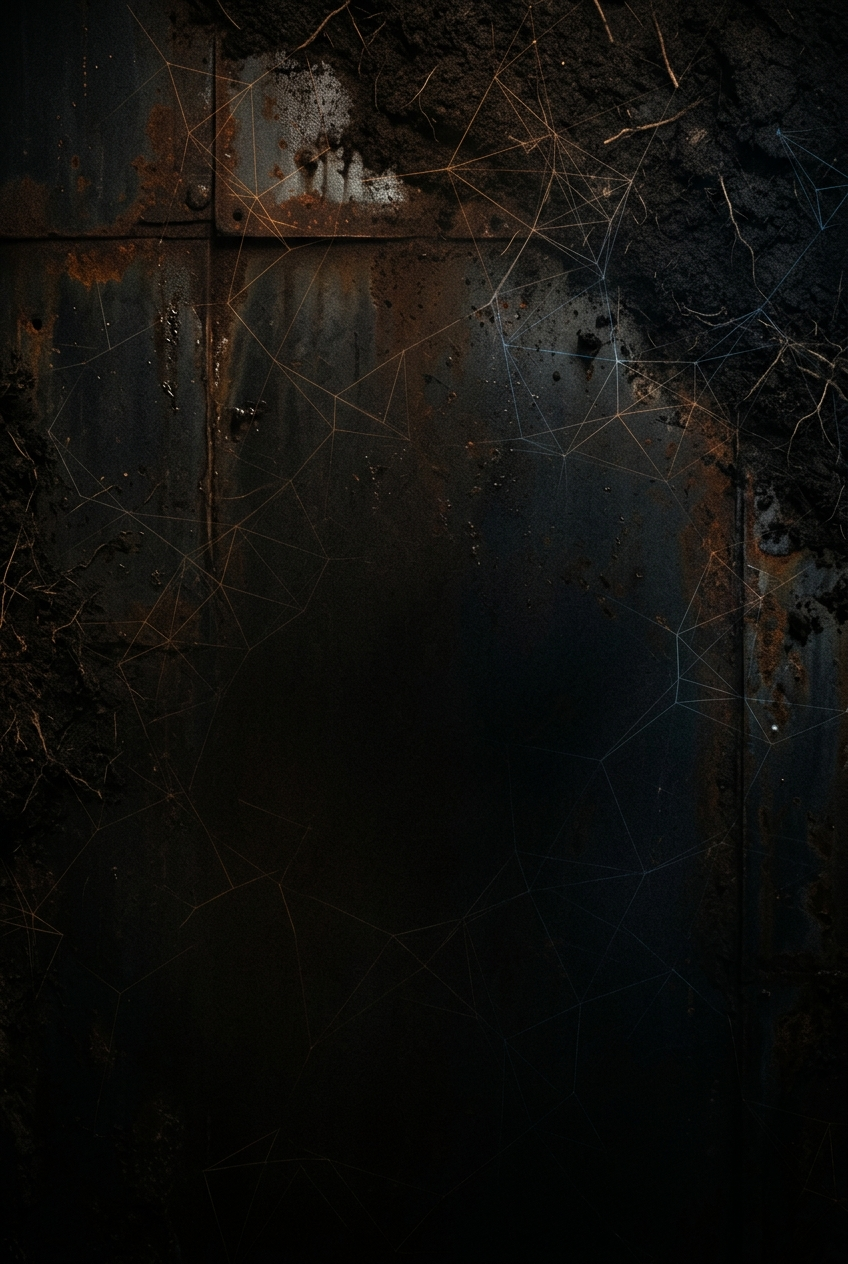
\includegraphics[width=\paperwidth, height=\paperheight]{backcover.png}
    }
}

% 2. Place the Text Overlay
\AddToShipoutPictureFG*{
    \AtPageLowerLeft{
        % Nudged to 0.15\paperheight and using [b] for bottom-anchor to keep it from climbing
        \put(\LenToUnit{0.1\paperwidth},\LenToUnit{0.15\paperheight}){
            \begin{minipage}[b][0.7\paperheight][c]{0.8\paperwidth}
                \color{signalGold}\setstretch{1.2}\headerfont

                \begin{center}
                    \fontsize{18}{22}\selectfont\textbf{THE BEAST IS DYING} \\
                    \fontsize{18}{22}\selectfont\textbf{THE LAND BREATHES AGAIN}
                \end{center}
                
                \vspace{4ex}

                \fontsize{10.5}{13}\selectfont
                The legacy world of fiat coercion, artificial scarcity, and bureaucratic violence is collapsing under its own thermodynamic weight. From the ashes of the old nation-state, a massive Polycentric Bioregional Commonwealth is rising.
                
                \vspace{2ex}
                Elara and Silas are stewards of the Foundry, a beating heart of steel and fire in a decentralized mesh of mutual aid. But when the dying beast of the legacy system lashes out to reclaim its lost territory through blockades, lawyers, and riot police, the true test of their society begins.
                
                \vspace{2ex}
                They must defend the physical reality of Layer 1 against the suffocating legalese of Layer 7, relying on the radical trust and restorative justice of the Sovereign Stack to hold the line. They will not be broken. They are building a civilization designed with \textbf{Fault Tolerance}.
                
                \vspace{4ex}

                \begin{center}
                    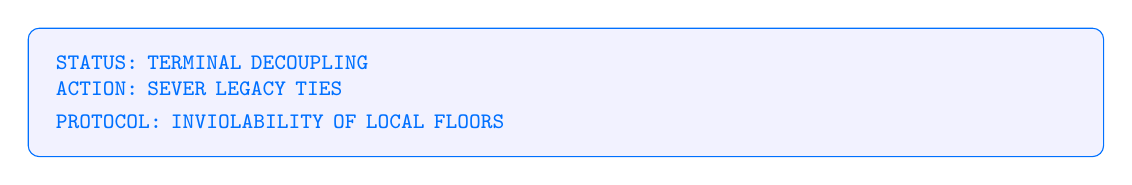
\begin{tikzpicture}
                        \node[draw=collectiveBlue, fill=blue!5, rounded corners, inner sep=10pt, text width=0.6\paperwidth, align=left] 
                        {\monofont\footnotesize\color{collectiveBlue} 
                            STATUS: TERMINAL DECOUPLING \\
                            ACTION: SEVER LEGACY TIES \\
                            PROTOCOL: INVIOLABILITY OF LOCAL FLOORS
                        };
                    \end{tikzpicture}
                \end{center}
                
                \vspace{4ex}

                \begin{center}
                    \fontsize{11}{14}\selectfont\textbf{A visceral, dirt-under-the-fingernails solarpunk epic.} \\
                    \fontsize{11}{14}\selectfont\textbf{The sequel to \textit{System Call}.}
                \end{center}

                \vspace{8ex}

                \begin{center}
                    \fontsize{10}{12}\selectfont
                    J.C. NOVAIS RAFFAINE \\ \url{github.com/raffaine/collective}
                \end{center}
            \end{minipage}
        }
    }
}
\newpage

\end{document}
